% ============================================================
%  The Particle Model — Lesson Booklet (one section per lesson: A Reading · B Theory · C Practice · D Above level)
%  Year 7 (Year 8 extension)  |  Victorian Curriculum F–10 Version 2.0
%  Compile with: xelatex three times, then python3 fill.py Particle_Model_Lesson_Booklet_Yr7
% ============================================================
\documentclass[11pt,a4paper]{article}

% ── Fonts (compile with LuaLaTeX) ────────────────────────────────────────────
\usepackage{fontspec}
% Bundled fonts (in ./fonts/) so the document compiles anywhere with XeLaTeX/LuaLaTeX
\setmainfont{Lato}[                   % body — humanist sans (stands in for deck's Inter)
  Path=./fonts/, Extension=.ttf, Ligatures=TeX,
  UprightFont=Lato-Regular, ItalicFont=Lato-Italic,
  BoldFont=Lato-Bold, BoldItalicFont=Lato-BoldItalic ]
\newfontfamily\headingfont{Poppins}[  % display/headings — matches the slide decks
  Path=./fonts/, Extension=.ttf, Ligatures=TeX,
  UprightFont=Poppins-Regular, ItalicFont=Poppins-Italic,
  BoldFont=Poppins-Bold, BoldItalicFont=Poppins-BoldItalic ]
\setlength{\headheight}{22pt}

\usepackage[protrusion=true,expansion=false]{microtype}
\usepackage[a4paper, top=2cm, bottom=2cm, left=2cm, right=2cm]{geometry}
\usepackage{xcolor}
\usepackage{tikz}
\usetikzlibrary{arrows.meta, shapes.geometric, calc, positioning, decorations.pathreplacing}
\usepackage{tcolorbox}
\tcbuselibrary{skins, breakable, raster}
\usepackage{fancyhdr}
\usepackage{titlesec}
\usepackage{enumitem}
\usepackage{booktabs}
\usepackage{tabularx}
\usepackage{array}
\usepackage{colortbl}
\usepackage{multicol}
\usepackage{amsmath}
\usepackage{needspace}
% TikZ diagram macros are embedded below (just before \begin{document}) for easy editing.
\usepackage{longtable}
\usepackage{lastpage}
\usepackage{calc}
\usepackage{mdframed}
\usepackage{setspace}
\usepackage{ragged2e}
% PDF bookmarks: one per lesson (made in \sectiondiv) plus the cover and
% contents, and links from the contents table to each lesson.
% implicit=false: hyperref adds no anchors of its own (an anchor on each
% list item nudged lists down 1.5 mm, which would undo the page fill).
% hidelinks keeps the links invisible, so the printed pages are unchanged.
\usepackage[implicit=false, hidelinks,
  pdftitle={The Particle Model — Lesson Booklet},
  pdfsubject={Years 7–8 Science, Victorian Curriculum F–10 v2.0}]{hyperref}
\usepackage{bookmark} % writes the outline itself, which implicit=false switches off in hyperref
% hyperref 7.01 with implicit=false leaves \Hy@PageAnchorSlide undefined, which
% throws at \end{document} and stops fill.py (it builds with -halt-on-error).
\makeatletter\providecommand\Hy@PageAnchorSlide{}\makeatother

% ── Colour Palette ───────────────────────────────────────────────────────────
% Remapped to the slide-deck palette (names kept so body + diagrams cascade)
\definecolor{NavyBlue}   {HTML}{16305C}
\definecolor{MidBlue}    {HTML}{2E6FE0}
\definecolor{LightBlue}  {HTML}{E8F1FF}
\definecolor{TealGreen}  {HTML}{0F6E63}
\definecolor{LightGreen} {HTML}{E0F7F3}
\definecolor{GoldDark}   {HTML}{C77F12}
\definecolor{GoldLight}  {HTML}{FFF3DC}
\definecolor{PurpleDark} {HTML}{5B3FC0}
\definecolor{PurpleLight}{HTML}{EFE9FF}
\definecolor{OrangeDark} {HTML}{C9483D}
\definecolor{OrangeLight}{HTML}{FFE9E6}
\definecolor{MidGrey}    {HTML}{AEBED4}
\definecolor{LightGrey}  {HTML}{F2F5FA}
\definecolor{DarkGrey}   {HTML}{3A4759}
\definecolor{TableHead}  {HTML}{16305C}
\definecolor{RowAlt}     {HTML}{EEF4FF}
% Bright accent tints (deck) for bars, rules and chips
\definecolor{Blue}   {HTML}{2E6FE0}
\definecolor{Teal}   {HTML}{18A999}
\definecolor{Amber}  {HTML}{F5A623}
\definecolor{Coral}  {HTML}{FF6B5E}
\definecolor{Violet} {HTML}{7C5CE0}
\definecolor{Sky}    {HTML}{4DA3FF}
\definecolor{Ink}    {HTML}{16223A}
\definecolor{Line}   {HTML}{DDE5F0}
\definecolor{Paper}  {HTML}{FBFCFE}

% ── Page Style ───────────────────────────────────────────────────────────────
\pagestyle{fancy}
\fancyhf{}
\renewcommand{\headrulewidth}{0.4pt}
\renewcommand{\headrule}{\hbox to\headwidth{\color{NavyBlue}\leaders\hrule height \headrulewidth\hfill}}
\fancyhead[L]{\headingfont\small\color{NavyBlue}The Particle Model}
\fancyhead[R]{\headingfont\small\color{DarkGrey}Year 7 \textbar{} Victorian Curriculum F--10 v2.0}
\fancyfoot[C]{\headingfont\small\color{DarkGrey}\thepage\ \textbar{} \pageref{LastPage}}
\fancypagestyle{plain}{%
  \fancyhf{}
  \fancyfoot[C]{\headingfont\small\color{DarkGrey}\thepage\ \textbar{} \pageref{LastPage}}
  \renewcommand{\headrulewidth}{0pt}
}

% ── Section Formatting ───────────────────────────────────────────────────────
\titleformat{\section}
  {\headingfont\color{NavyBlue}\Large\bfseries}
  {}{0em}{}
  [{\color{Teal}\rule[0.6ex]{2.2em}{3pt}}{\color{Line}\rule[0.6ex]{\dimexpr\linewidth-2.2em\relax}{1pt}}]
\titlespacing{\section}{0pt}{18pt}{8pt}

\titleformat{\subsection}
  {\headingfont\color{MidBlue}\large\bfseries}
  {\thesubsection}{0.6em}{}
\titlespacing{\subsection}{0pt}{12pt}{4pt}

\titleformat{\subsubsection}
  {\headingfont\color{NavyBlue}\normalsize\bfseries}
  {}{0em}{}
\titlespacing{\subsubsection}{0pt}{8pt}{2pt}

% Deck-style eyebrow / kicker (optional use)
\newcommand{\kicker}[2][Teal]{%
  {\headingfont\bfseries\footnotesize\color{#1}%
   \textcolor{#1}{\rule[0.18ex]{1.6em}{2.2pt}}\hspace{0.5em}\MakeUppercase{#2}\par}%
  \vspace{2pt}}

% ── Custom tcolorbox Environments ────────────────────────────────────────────

% Section divider banner
\newtcolorbox{sectionbanner}[2]{
  enhanced, breakable=false,
  colback=NavyBlue, colframe=NavyBlue,
  fontupper=\color{white}\bfseries\large,
  left=4mm, right=4mm, top=3mm, bottom=3mm,
  title={\color{white}\Huge\bfseries #1},
  attach boxed title to top left={yshift=-2mm, xshift=4mm},
  boxed title style={colback=NavyBlue, colframe=NavyBlue},
  after upper={\par\smallskip\normalfont\normalsize\color{white!80!NavyBlue}\textit{#2}}
}

% Key info box (blue)
\newtcolorbox{infobox}[1]{
  breakable, arc=2.5mm, boxrule=0.5pt,
  colback=LightBlue, colframe=Blue!40,
  fonttitle=\headingfont\bfseries, coltitle=MidBlue,
  title={#1},
  left=4mm, right=3.5mm, top=2.5mm, bottom=2.5mm
}

% Scaffold box (yellow)
\newtcolorbox{scaffold}[1]{
  breakable, arc=2.5mm, boxrule=0.5pt,
  colback=GoldLight, colframe=Amber!40,
  fonttitle=\headingfont\bfseries, coltitle=GoldDark,
  title={#1},
  left=4mm, right=3.5mm, top=2.5mm, bottom=2.5mm
}

% Worked example box
\newtcolorbox{workedexbox}[1]{
  breakable, arc=2.5mm, boxrule=0.5pt,
  colback=white, colframe=Amber!50,
  fonttitle=\headingfont\bfseries, coltitle=GoldDark,
  title={#1},
  left=4mm, right=3.5mm, top=2.5mm, bottom=2.5mm
}
% Worked examples: \begin{workedex}{title} -> "Worked Example N.M --- title",
% auto-numbered per section and labelled we:N.M. Never type the number.
\newcounter{wenum}[section]
\renewcommand{\thewenum}{\thesection.\arabic{wenum}}
\newenvironment{workedex}[1]
  {\refstepcounter{wenum}\label{we:\thewenum}\begin{workedexbox}{Worked Example \thewenum\ --- #1}}
  {\end{workedexbox}}

% We do: straight after each worked example, a near-identical question the
% class works through together, with its own writing space. Numbered to
% match the worked example above it and labelled wd:N.M.
%   \begin{wedo}{title} question ... \answerbox{h} \end{wedo}
\newtcolorbox{wedobox}[1]{
  enhanced, breakable=false, arc=2.5mm, boxrule=0.5pt,
  colback=white, colframe=TealGreen!55,
  fonttitle=\headingfont\bfseries, coltitle=TealGreen!75!black,
  title={#1},
  left=4mm, right=3.5mm, top=2.5mm, bottom=2.5mm
}
\newenvironment{wedo}[1]
  {\par\needspace{9\baselineskip}\begin{wedobox}{We do \thewenum\ --- #1}\label{wd:\thewenum}\ignorespaces}
  {\end{wedobox}}

% Year 7 box (blue)
\newtcolorbox{yr7box}{
  breakable, arc=2.5mm, boxrule=0.5pt,
  colback=LightBlue, colframe=Blue!40,
  left=4mm, right=3.5mm, top=2.5mm, bottom=2.5mm
}

% Year 8 extension box (violet)
\newtcolorbox{yr8box}{
  breakable, arc=2.5mm, boxrule=0.5pt,
  colback=PurpleLight, colframe=Violet!40,
  left=4mm, right=3.5mm, top=2.5mm, bottom=2.5mm
}

% Answer lines box
\newcommand{\answerbox}[1]{%
  \begin{tcolorbox}[
    enhanced, breakable, arc=2mm,
    colback=Paper, colframe=Line,
    left=2mm, right=2mm, top=1mm, bottom=1mm,
    boxrule=1pt,
    height=#1
  ]
  \end{tcolorbox}%
}

% Experiment header
\newtcolorbox{expheader}[3]{
  breakable=false, arc=2.5mm,
  colback=RowAlt, colframe=Amber!50, boxrule=0.5pt,
  fonttitle=\headingfont\bfseries\large, coltitle=NavyBlue,
  title={Experiment #1: #2},
  left=4mm, right=3.5mm, top=2.5mm, bottom=2.5mm,
  after upper={\par\smallskip
    {\headingfont\bfseries\color{GoldDark}Aim:}\ \textit{#3}},
}

% Reading comprehension passage box (green)
\newtcolorbox{readingbox}[1]{
  breakable, arc=2.5mm, boxrule=0.5pt,
  colback=white, colframe=Teal!50,
  fonttitle=\headingfont\bfseries, coltitle=TealGreen,
  title={#1},
  left=4mm, right=3.5mm, top=2.5mm, bottom=2.5mm,
  fontupper=\normalsize
}

% Skill-builder box (for beginner scaffolding)
\newtcolorbox{skillbox}[1]{
  breakable, arc=2.5mm, boxrule=0.5pt,
  colback=RowAlt, colframe=Blue!40,
  fonttitle=\headingfont\bfseries, coltitle=MidBlue,
  title={#1},
  left=4mm, right=3.5mm, top=2.5mm, bottom=2.5mm
}

% ── Custom Commands ───────────────────────────────────────────────────────────

% Question: \question{marks}{text}  (marks can be empty)
% Numbered automatically as Q<section>.<n>, reset every section.
% Do NOT write numbers by hand.
\newcounter{qnum}[section]
\renewcommand{\theqnum}{\thesection.\arabic{qnum}}
\newcommand{\question}[2]{%
  \refstepcounter{qnum}%
  \needspace{3\baselineskip}%
  \medskip
  \noindent\label{q:\theqnum}\textbf{Q\theqnum}\ifx&#1&\else\ \textcolor{DarkGrey}{(#1 mark\ifnum#1=1\else s\fi)}\fi\quad #2%
  \medskip
}

% Inline marks note
\newcommand{\markscount}[1]{\hfill\textcolor{DarkGrey}{\textit{(#1 mark\ifnum#1=1\else s\fi)}}}

% ── Practice set counter and question macros ─────────────────────────────────
\newcounter{pqnum}
\newcommand{\practiceset}[1]{%
  \needspace{6\baselineskip}
  \setcounter{pqnum}{0}%
  \vspace{6pt}
  {\headingfont\bfseries\large\color{GoldDark} Practice Set --- #1}\\[-2pt]
  {\color{Amber}\rule{\linewidth}{1pt}}\\[2pt]
}
% \pq{question text}{working box height}
\newcommand{\pq}[2]{%
  \stepcounter{pqnum}%
  \needspace{4\baselineskip}
  \vspace{5pt}
  \noindent\textbf{\thepqnum.}\quad #1\par
  \vspace{2pt}
  \answerbox{#2}
}
% Two short questions side by side, each with its own box
\newcommand{\pqpair}[4]{%
  \needspace{4\baselineskip}
  \vspace{5pt}
  \noindent
  \begin{minipage}[t]{0.48\linewidth}
    \stepcounter{pqnum}\textbf{\thepqnum.}\quad #1\par\vspace{2pt}
    \begin{tcolorbox}[enhanced,arc=2mm,colback=Paper,colframe=Line,left=2mm,right=2mm,
      top=1mm,bottom=1mm,boxrule=1pt,height=#2]\end{tcolorbox}
  \end{minipage}\hfill
  \begin{minipage}[t]{0.48\linewidth}
    \stepcounter{pqnum}\textbf{\thepqnum.}\quad #3\par\vspace{2pt}
    \begin{tcolorbox}[enhanced,arc=2mm,colback=Paper,colframe=Line,left=2mm,right=2mm,
      top=1mm,bottom=1mm,boxrule=1pt,height=#4]\end{tcolorbox}
  \end{minipage}
}

% ── Comprehension question macro (compact, lined) ────────────────────────────
\newcounter{rcnum}
\newcommand{\rcreset}{\setcounter{rcnum}{0}}
\newcommand{\rcq}[2]{%
  \stepcounter{rcnum}%
  \needspace{3\baselineskip}
  \vspace{4pt}
  \noindent\textbf{C\thercnum.}\quad #1\par
  \vspace{2pt}
  \linedbox{#2}
}

% Section divider (big numbered banner): \sectiondiv{title}{summary}
%
% This IS the section: it steps the real section counter, so subsections,
% tasks, questions and figures inside it are numbered N.M automatically.
% Put \label{sec:N} straight after it. Never hand-type a section number.
\newcommand{\sectiondiv}[2]{%
  \needspace{5\baselineskip}%
  \refstepcounter{section}%
  % PDF bookmark for the lesson; its anchor, lesson.N.1, is what the contents table links to
  \pdfbookmark[1]{Lesson \thesection{} — #1}{lesson.\thesection}%
  \begin{tcolorbox}[
    enhanced, breakable=false, arc=3.5mm,
    colback=NavyBlue, colframe=NavyBlue, boxrule=0pt,
    sidebyside, sidebyside align=center,
    lefthand width=2.4cm,
    left=2mm, right=4mm, top=4mm, bottom=4mm
  ]
    \begin{center}
      {\headingfont\bfseries\color{white!35!NavyBlue}\fontsize{50}{50}\selectfont \thesection}
    \end{center}
    \tcblower
    {\headingfont\bfseries\color{white}\LARGE #1}\\[3pt]
    {\itshape\color{white!75!NavyBlue}\small #2}
  \end{tcolorbox}%
}

% Tasks: \task, \task[a] (part a of a NEW task), \taskpart{b} (next part
% of the same task), \exttask (Year 8 "Extension" — same counter).
% Numbered Task <section>.<n>, reset every section. Do NOT type numbers.
% Every task, question and figure also gets an automatic label
% (task:1.7b, q:2.4, fig:1.2, fig:E2.1) so page refs come from the .aux.
\newcounter{tasknum}[section]
\renewcommand{\thetasknum}{\thesection.\arabic{tasknum}}
\NewDocumentCommand{\task}{o}{\refstepcounter{tasknum}\label{task:\thetasknum\IfValueT{#1}{#1}}\textbf{Task \thetasknum\IfValueT{#1}{#1}}}
\newcommand{\taskpart}[1]{\label{task:\thetasknum#1}\textbf{Task \thetasknum#1}}
\newcommand{\exttask}{\refstepcounter{tasknum}\label{task:\thetasknum}\textbf{Extension \thetasknum}}

% Figure captions: \figcap[fig:label]{caption} -> "Figure N.M --- caption"
% \expfigcap{caption} -> "Figure EN.M" (experiment pages). Both auto-numbered.
\newcounter{fignum}[section]
\renewcommand{\thefignum}{\thesection.\arabic{fignum}}
\newcounter{expfignum}[section]
\renewcommand{\theexpfignum}{E\thesection.\arabic{expfignum}}
\newcommand{\figcap}[2][]{%
  \begin{center}
    \refstepcounter{fignum}\label{fig:\thefignum}\if\relax\detokenize{#1}\relax\else\label{#1}\fi
    \small\itshape\color{DarkGrey} Figure \thefignum\ --- #2
  \end{center}%
}
\newcommand{\expfigcap}[1]{%
  \begin{center}
    \refstepcounter{expfignum}\label{fig:\theexpfignum}%
    \small\itshape\color{DarkGrey} Figure \theexpfignum\ --- #1
  \end{center}%
}

% Diagram include
\newcommand{\diagramfig}[3]{%  {filename}{width fraction}{caption}
  \begin{center}
    \includegraphics[width=#2\linewidth]{#1}\\[4pt]
    \small\itshape\color{DarkGrey} #3
  \end{center}%
}

% Table column types
\newcolumntype{L}[1]{>{\RaggedRight\arraybackslash}p{#1}}
\newcolumntype{C}[1]{>{\Centering\arraybackslash}p{#1}}

% Table header colour
\newcommand{\thead}[1]{\cellcolor{TableHead}\color{white}\bfseries #1}
\newcommand{\talt}{\rowcolor{RowAlt}}
\newcommand{\tmid}{\rowcolor{MidGrey}}

% Inline year tags
\newcommand{\tagyr}[1]{%
  \tikz[baseline=-0.5ex]\node[
    rounded corners=2pt,
    fill=#1!20, draw=#1, text=#1,
    inner xsep=4pt, inner ysep=1pt,
    font=\scriptsize\bfseries
  ]{Yr #1 only};}

% Draw answer lines
\newcommand{\anslines}[1]{%
  \vspace{2pt}%
  \foreach \n in {1,...,#1}{%
    \par\noindent\rule{\linewidth}{0.3pt}\vspace{3pt}%
  }%
}

% ── Document ─────────────────────────────────────────────────────────────────
% ── Optional-lesson note, shown under the lesson banner ──────────────────────
\newcommand{\optionalnote}[1]{%
  % the title is a bold lead-in on the first line rather than a title bar,
  % which keeps Lesson 11's reading on the lesson's first page
  \begin{tcolorbox}[enhanced, breakable=false, arc=2.5mm, boxrule=0.5pt,
    colback=PurpleLight, colframe=Violet!50,
    left=4mm, right=3.5mm, top=2mm, bottom=2mm]
  {\headingfont\bfseries\color{PurpleDark}Optional lesson \textbullet{} Year 8 extension.}\enspace #1
  \end{tcolorbox}\vspace{2pt}}


% ══════════════════════════════════════════════════════════════════════════════
%  LESSON STRUCTURE (lesson booklet, Oct 2026)
%  Every lesson runs in the same four parts, in this order:
%    \lessonpart{A}{Reading and comprehension}{Teal}   \label{read:N}
%    \lessonpart{B}{Theory and examples}{Blue}         \label{theory:N}
%    \lessonpart{C}{Practice}{Amber}                    \label{prac:N}
%    \lessonpart{D}{Above level}{Violet}                \label{ext:N}
%  Above-level / higher-order questions live ONLY in Part D, at the end.
% ══════════════════════════════════════════════════════════════════════════════
\newcommand{\lessonpart}[3]{%
  \par\if#1A\needspace{10\baselineskip}\vspace{10pt}\else
    \if#1C\notesfill\fi\clearpage\fi
  \begin{tcolorbox}[enhanced, breakable=false, arc=2mm, boxrule=0pt,
    colback=#3!14, borderline west={4pt}{0pt}{#3},
    left=4mm, right=3mm, top=1.6mm, bottom=1.6mm]
  {\headingfont\bfseries\color{#3!60!black}\large Part #1 \textbullet{} #2}
  \end{tcolorbox}\vspace{2pt}}

% Key vocabulary at the start of each lesson: students copy each definition
% from the vocabulary slide in the lesson's starter. First row = red scaffold.
\newcommand{\vocabhead}{%
  \par\vspace{6pt}%
  \begin{tcolorbox}[enhanced, breakable=false, arc=2mm, boxrule=0pt,
    colback=NavyBlue!10, borderline west={4pt}{0pt}{NavyBlue},
    left=4mm, right=3mm, top=1.6mm, bottom=1.6mm]
  {\headingfont\bfseries\color{NavyBlue}\large Key vocabulary}
  \end{tcolorbox}\vspace{2pt}%
  \noindent Copy the definition of each word from the slide. The first one has been done for you.\par}

% Curriculum codes under a lesson banner
\newcommand{\lessoncodes}[1]{%
  {\small\headingfont\color{DarkGrey}Victorian Curriculum 2.0:\ \textbf{#1}}\par\vspace{4pt}}

% Two short tasks side by side, each with its own working box
% \taskpair{text}{box height}{text}{box height}
% The two boxes line up: the shorter question is padded by the difference in
% text height (measured in a scratch box, task counter restored, no label).
\newsavebox\tpbox
\newlength\tpA \newlength\tpB
\newcount\tpsaved
\newcommand\tpmeasure[2]{%
  \tpsaved=\value{tasknum}%
  \sbox\tpbox{\vbox{\hsize=0.485\linewidth \linewidth=\hsize \parskip=0pt
    \renewcommand\label[1]{}\task #1\par}}%
  \setlength{#2}{\dimexpr\ht\tpbox+\dp\tpbox\relax}%
  \setcounter{tasknum}{\tpsaved}}
\newcommand{\taskpair}[4]{%
  \par\needspace{9\baselineskip}\vspace{4pt}%
  \tpmeasure{#1}{\tpA}\tpmeasure{#3}{\tpB}%
  \noindent
  \edef\abgrp{\number\numexpr\value{abox}+1\relax}%
  \begin{minipage}[t]{0.485\linewidth}
    \task #1\par\ifdim\tpB>\tpA\vspace{\dimexpr\tpB-\tpA\relax}\fi\vspace{2pt}\answerbox{#2}
  \end{minipage}\hfill
  \begin{minipage}[t]{0.485\linewidth}
    \task #3\par\ifdim\tpA>\tpB\vspace{\dimexpr\tpA-\tpB\relax}\fi\vspace{2pt}\answerbox{#4}
  \end{minipage}\par\gdef\abgrp{0}\vspace{4pt}}
% Two parts of one question side by side, with their answer boxes level:
% \ptpair{a}{part (a) text}{box height}{b}{part (b) text}{box height}.
% The shorter part's text gets space below it to match the longer one.
\newcommand\ptmeasure[3]{%
  \sbox\tpbox{\vbox{\hsize=0.485\linewidth \linewidth=\hsize \parskip=0pt \pt{#1}#2\par}}%
  \setlength{#3}{\dimexpr\ht\tpbox+\dp\tpbox\relax}}
\newcommand{\ptpair}[6]{%
  \ptmeasure{#1}{#2}{\tpA}\ptmeasure{#4}{#5}{\tpB}%
  \par\noindent
  \edef\abgrp{\number\numexpr\value{abox}+1\relax}%
  \begin{minipage}[t]{0.485\linewidth}
    \pt{#1}#2\par\ifdim\tpB>\tpA\vspace{\dimexpr\tpB-\tpA\relax}\fi\answerbox{#3}
  \end{minipage}\hfill
  \begin{minipage}[t]{0.485\linewidth}
    \pt{#4}#5\par\ifdim\tpA>\tpB\vspace{\dimexpr\tpA-\tpB\relax}\fi\answerbox{#6}
  \end{minipage}\par\gdef\abgrp{0}}

% Answer boxes never split across a page (a half box on its own page is useless)
% ── Page filling ────────────────────────────────────────────────────────────
% Every writing box gets an id. Its page is logged to \jobname.abp; fill.py
% measures the empty space left at the foot of each page and shares it out
% among that page's boxes via \jobname.abx (\abset{id}{extra}). Side-by-side
% boxes share a group so they grow together.
\newcounter{abox}
\newwrite\abpos \immediate\openout\abpos=\jobname.abp
\newcommand{\abset}[2]{\expandafter\gdef\csname abx@#1\endcsname{#2}}
\InputIfFileExists{\jobname.abx}{}{}
\def\abgrp{0}
\newcommand{\abnext}{\stepcounter{abox}%
  \edef\abcur{\ifcsname abx@\theabox\endcsname\csname abx@\theabox\endcsname\else 0pt\fi}}
\newcommand{\ablog}{\edef\abtmp{\noexpand\write\abpos{\theabox\space\abgrp\space\noexpand\thepage}}\abtmp}
\newcommand{\abh}[1]{\dimexpr#1+\abcur\relax}
\renewcommand{\answerbox}[1]{%
  \abnext
  \begin{tcolorbox}[enhanced, breakable=false, arc=2mm, colback=Paper, colframe=Line,
    left=2mm, right=2mm, top=1mm, bottom=1mm, boxrule=1pt, height=\abh{#1}]
  \end{tcolorbox}\ablog%
}
% \linedbox{height}: an answer box ruled in dotted thirds. Lines are \thirdrow/3 apart and run dotted, dotted,
% solid (the baseline), repeating, and end on one dotted line. The number of
% rows is worked out from the box's final height, so the ruling still fills the
% box after fill.py has grown it; the rows are centred in the box.
\newlength\thirdrow \setlength\thirdrow{9mm}
\tikzset{thirdsolid/.style={draw=DarkGrey!70, line width=0.5pt},
         thirddot/.style={draw=DarkGrey!70, line width=0.6pt, dash pattern=on 0.9pt off 1.6pt}}
\newlength\lbH \newlength\lbO \newcount\lbN
\newcommand{\linedbox}[1]{%
  \abnext
  % interior height = box height less the 1pt frame top and bottom
  \setlength\lbH{\dimexpr\abh{#1}-2pt\relax}%
  % whole rows that fit with at least 3 mm spare top and bottom (at least one)
  \lbN=\numexpr(\dimexpr\lbH-6mm-\thirdrow/2\relax)/\thirdrow\relax
  \ifnum\lbN<1 \lbN=1 \fi
  \setlength\lbO{\dimexpr(\lbH-\lbN\thirdrow)/2\relax}%
  \begin{tcolorbox}[enhanced, breakable=false, arc=2mm, colback=Paper, colframe=Line,
    left=2mm, right=2mm, top=1mm, bottom=1mm, boxrule=1pt, height=\abh{#1},
    underlay={\begin{tcbclipinterior}
      \foreach \i in {1,...,\the\lbN}{
        \draw[thirddot] ([xshift=3mm,yshift=-\lbO-(\i-1)*\thirdrow]interior.north west) -- ([xshift=-3mm,yshift=-\lbO-(\i-1)*\thirdrow]interior.north east);
        \draw[thirddot] ([xshift=3mm,yshift=-\lbO-(\i-1)*\thirdrow-\thirdrow/3]interior.north west) -- ([xshift=-3mm,yshift=-\lbO-(\i-1)*\thirdrow-\thirdrow/3]interior.north east);
        \draw[thirdsolid] ([xshift=3mm,yshift=-\lbO-(\i-1)*\thirdrow-2*\thirdrow/3]interior.north west) -- ([xshift=-3mm,yshift=-\lbO-(\i-1)*\thirdrow-2*\thirdrow/3]interior.north east);}
      \draw[thirddot] ([xshift=3mm,yshift=-\lbO-\lbN\thirdrow]interior.north west) -- ([xshift=-3mm,yshift=-\lbO-\lbN\thirdrow]interior.north east);
    \end{tcbclipinterior}}]
  \end{tcolorbox}\ablog%
}
% Every written-response box is ruled the same way (Part A comprehension, We do,
% Part C tasks and Part D extensions, including side-by-side pairs). Space for
% mathematical working uses \workbox{height} instead and stays plain, as do
% \drawbox and the write-in tables.
\let\workbox\answerbox   % plain box: mathematical working (calculations) stays unruled
\let\answerbox\linedbox
% \drawbox{height}{contents}: white box for a diagram or drawing
\newcommand{\drawbox}[2]{%
  \abnext
  \begin{tcolorbox}[colback=white, colframe=MidGrey, boxrule=0.5pt, height=\abh{#1}]#2\end{tcolorbox}\ablog}
% Notes box at the end of Part B: fills whatever is left of the page (if worth it)
\newcommand{\notesfill}{\par
  \ifdim\dimexpr\pagegoal-\pagetotal\relax>3.2cm
    \vspace*{\fill}%
    \begin{tcolorbox}[enhanced, breakable=false, arc=2mm, colback=Paper, colframe=Line,
      left=2mm, right=2mm, top=1mm, bottom=1mm, boxrule=1pt,
      height=\dimexpr\pagegoal-\pagetotal-1.0cm\relax]
      {\small\headingfont\color{DarkGrey}Notes}
    \end{tcolorbox}%
  \fi}



% Centred table: wrap every content table in \begin{ctab} ... \end{ctab}
% (figures already centre themselves inside their \diag... macros)
% ctab also registers write-in tables (S column) for page filling: the extra
% height is per row, logged with the row count.
\newenvironment{ctab}{\par\smallskip\begingroup\centering
  \abnext\let\tbcur\abcur\global\wtrows0 }{\par
  \ifnum\wtrows>0 \edef\abtmp{\noexpand\write\abpos{\theabox\space\abgrp\space\noexpand\thepage\space\the\wtrows}}\abtmp\fi
  \endgroup\smallskip}

% ── Booklet formatting rules (Oct 2026) ─────────────────────────────────────
% 1. No marks are shown anywhere in the booklet.
\renewcommand{\markscount}[1]{}
% 2. A task's heading sits on its own line; its text starts on the next
%    line, left aligned. Parts (a), (b)… each start a new line: use \pt{a}.
\RenewDocumentCommand{\task}{o}{\par\noindent\refstepcounter{tasknum}\label{task:\thetasknum\IfValueT{#1}{#1}}\textbf{Task \thetasknum\IfValueT{#1}{#1}}\par\nobreak\noindent\ignorespaces}
\renewcommand{\taskpart}[1]{\par\noindent\label{task:\thetasknum#1}\textbf{Task \thetasknum#1}\par\nobreak\noindent\ignorespaces}
\renewcommand{\exttask}{\par\noindent\refstepcounter{tasknum}\label{task:\thetasknum}\textbf{Extension \thetasknum}\par\nobreak\noindent\ignorespaces}
\newcommand{\pt}[1]{\par\noindent\textbf{(#1)}\ \ignorespaces}
% Workstation pages (Experiment 1): numbered method steps with a hanging
% indent, and a one-line safety reminder under the materials list.
\newcommand{\wsstep}[1]{\par\noindent\hangindent=1.6em\hangafter=1\makebox[1.6em][l]{\textbf{#1}}\ignorespaces}
\newcommand{\wssafety}[1]{\par\smallskip{\small\textcolor{ScaffoldRed}{\headingfont\bfseries Safety:}\ #1}\par}
% 3. Tables have vertical rules between columns and down both sides
%    (write | between and around the columns, e.g. {|L{3cm}|C{2cm}|}).
%    Keep the normal padding at the outer edges (no @{} there): colortbl paints
%    header colour one \tabcolsep past each edge, so trimming the padding makes
%    the header overhang the grid.
\arrayrulecolor{MidGrey}
\setlength{\arrayrulewidth}{0.6pt}
% 4. Write-in tables: W/Z are left/centred columns that centre text
%    vertically; put the S column first (see below).
\newcolumntype{W}[1]{>{\RaggedRight\arraybackslash}m{#1}}
\newcolumntype{Z}[1]{>{\Centering\arraybackslash}m{#1}}
\def\tbcur{0pt}
\newcount\wtrows
\newcommand{\wh}{\global\advance\wtrows1 \rule[\dimexpr-0.75cm-\tbcur/2\relax]{0pt}{\dimexpr1.5cm+\tbcur\relax}}
% S = zero-width first column that makes every row of a write-in table
% at least 1.5 cm tall with its text vertically centred. Start each data
% row with "&"; start the header row with "\hd &" so it stays slim.
\newif\ifnowh
\newcolumntype{S}{@{}>{}c<{\ifnowh\else\wh\fi\global\nowhfalse}@{\hspace{\tabcolsep}}}
\newcommand{\hd}{\global\nowhtrue}
% 5. The first row of a multi-row write-in table is a worked scaffold in red.
\definecolor{ScaffoldRed}{HTML}{C0392B}
\newcommand{\scaf}[1]{\textcolor{ScaffoldRed}{\itshape #1}}
% 6. Tables are a light grid (rules between rows and columns) on white —
%    row shading is off, because colortbl paints shading over column rules.
\renewcommand{\talt}{}
\renewcommand{\tmid}{}
% ══════════════════════════════════════════════════════════════════════════════
%  DIAGRAM DEFINITIONS — The Particle Model
%  Self-contained TikZ macros, no external image files. Each \diag... macro is
%  called from the body by name.
% ══════════════════════════════════════════════════════════════════════════════
\usetikzlibrary{arrows.meta,calc,positioning,patterns,backgrounds}
\tikzset{
  thin arrow/.style={-{Stealth[length=6pt,width=4pt]}, line width=1.4pt},
}

% ── Lesson 1: the same three jars holding a solid, a liquid and a gas ───────────
% The solid keeps its own shape, the liquid takes the jar's shape with a flat top,
% the gas fills the whole jar. No particles yet: those arrive in Lesson 4.
\newcommand{\jar}[1]{% jar outline with its base at (#1,0)
  \draw[line width=1.2pt, Ink] (#1-1.25,2.9) -- (#1-1.25,0.15) arc (180:270:0.15)
    -- (#1+1.1,0) arc (270:360:0.15) -- (#1+1.25,2.9);}
\newcommand{\diagStates}{%
\begin{center}
\begin{tikzpicture}[font=\small, x=1cm, y=1cm]
  % solid: a block sitting in the corner
  \fill[GoldLight] (-0.95,0.02) rectangle (0.15,1.25);
  \draw[GoldDark, line width=1.1pt] (-0.95,0.02) rectangle (0.15,1.25);
  \jar{0}
  \node[font=\bfseries, text=NavyBlue] at (0,-0.45) {Solid};
  \node[align=center, font=\footnotesize, text=DarkGrey] at (0,-1.05) {keeps its own shape\\and volume};
  % liquid: takes the jar's shape, flat top
  \begin{scope}[xshift=4.2cm]
    \fill[Sky!35] (-1.25,0.15) arc (180:270:0.15) -- (1.1,0) arc (270:360:0.15) -- (1.25,1.1) -- (-1.25,1.1) -- cycle;
    \draw[MidBlue, line width=1.1pt] (-1.25,1.1) -- (1.25,1.1);
    \jar{0}
    \node[font=\bfseries, text=NavyBlue] at (0,-0.45) {Liquid};
    \node[align=center, font=\footnotesize, text=DarkGrey] at (0,-1.05) {takes the jar's shape,\\keeps its volume};
  \end{scope}
  % gas: fills the whole (sealed) jar
  \begin{scope}[xshift=8.4cm]
    \fill[Violet!16] (-1.25,0.15) arc (180:270:0.15) -- (1.1,0) arc (270:360:0.15) -- (1.25,2.9) -- (-1.25,2.9) -- cycle;
    \draw[line width=2.2pt, DarkGrey] (-1.4,2.9) -- (1.4,2.9);
    \jar{0}
    \node[font=\scriptsize, text=DarkGrey, anchor=south] at (0,2.95) {lid};
    \node[font=\bfseries, text=NavyBlue] at (0,-0.45) {Gas};
    \node[align=center, font=\footnotesize, text=DarkGrey] at (0,-1.05) {spreads out to fill\\the whole jar};
  \end{scope}
\end{tikzpicture}
\end{center}}

% ── Lesson 1, Worked Example 1.2 and We do 1.2: the same syringe, before and after
\newcommand{\diagSyringe}[3]{% {start mL}{end mL}{contents: gas|liquid}
\begin{center}\resizebox{\linewidth}{!}{%
\begin{tikzpicture}[font=\scriptsize, x=0.11cm, y=1cm]
  \foreach \row/\vol/\lab in {0/#1/before, -1.15/#2/after}{
    \begin{scope}[yshift=\row cm]
      \ifx#3g\fill[Violet!16] (0,0) rectangle (\vol,0.7);\else\fill[Sky!35] (0,0) rectangle (\vol,0.7);\fi
      \draw[line width=1pt, Ink] (0,0) rectangle (60,0.7);
      \draw[line width=1pt, Ink] (0,0.25) -- (-4,0.25) (0,0.45) -- (-4,0.45);
      \fill[Ink] (-5.5,0.15) rectangle (-4,0.55);
      \foreach \t in {0,10,...,60}{\draw[Ink] (\t,0.7) -- (\t,0.85); \node[anchor=south, font=\tiny] at (\t,0.82) {\t};}
      \fill[DarkGrey] (\vol,0.04) rectangle (\vol+1.6,0.66);
      \draw[line width=2pt, DarkGrey] (\vol+1.6,0.35) -- (\vol+26,0.35);
      \draw[line width=2pt, DarkGrey] (\vol+26,0.05) -- (\vol+26,0.65);
      \node[anchor=east, font=\scriptsize\bfseries, text=DarkGrey] at (-7,0.35) {\lab};
    \end{scope}}
  \node[font=\tiny, text=DarkGrey, anchor=west] at (61,0.35) {mL};
  \node[font=\tiny, text=DarkGrey, anchor=north] at (-4.75,-1.2) {sealed tip};
\end{tikzpicture}}
\end{center}}

% needspace.sty reserves room by planting a penalty -100 with 9 lines of
% temporary stretch. On a page that can't be filled tightly that fake break
% always wins, so a We do that fitted was pushed over and left half a page
% empty. This version breaks only when the room really isn't there, and
% ragged bottom lets every other page run on until something won't fit;
% fill.py then grows the writing boxes into what is left at the foot.
\renewcommand{\needspace}[1]{\par\ifdim\dimexpr\pagegoal-\pagetotal\relax<\dimexpr#1\relax\newpage\fi}
\raggedbottom
% Part D sits in a breakable yr8box, where \needspace can't see the page (the box
% is built off the page first). Wrap each extension in keepext so it is one
% unsplittable block: the yr8box then breaks between extensions, never inside one.
\newenvironment{keepext}{\par\begin{tcolorbox}[blankest, breakable=false]}{\end{tcolorbox}\par}
% ══════════════════════════════════════════════════════════════════════════════
%  SHARED DIAGRAMS — particle boxes, graphs and lab apparatus (Lessons 2–27)
% ══════════════════════════════════════════════════════════════════════════════
% Particles are 3.2 mm discs. Solids and liquids hold about the same number of
% particles at the same spacing (touching): a liquid is NOT drawn more spread
% out than a solid, because that is the misconception Lesson 6 corrects.
\tikzset{
  pA/.style={circle, fill=Sky!55, draw=MidBlue, line width=0.5pt, minimum size=3.2mm, inner sep=0pt},
  pB/.style={circle, fill=Coral!50, draw=OrangeDark, line width=0.5pt, minimum size=3.2mm, inner sep=0pt},
  pC/.style={circle, fill=Amber!55, draw=GoldDark, line width=0.5pt, minimum size=3.2mm, inner sep=0pt},
  pD/.style={circle, fill=Teal!45, draw=TealGreen, line width=0.5pt, minimum size=3.2mm, inner sep=0pt},
  move/.style={-{Stealth[length=3pt,width=3pt]}, line width=0.7pt, DarkGrey},
  boxline/.style={line width=1pt, Ink},
  axis/.style={-{Stealth[length=5pt,width=4pt]}, line width=0.9pt, Ink},
  glass/.style={line width=1pt, Ink},
  lab/.style={font=\scriptsize, text=DarkGrey},
}
\makeatletter
% particle kinds, drawn at (#1,#2): A, B, C, D single particles; AA, BB, CC
% two joined; AB a joined pair; BAB a three-particle molecule.
\newcommand{\pk@A}[2]{\node[pA] at (#1,#2) {};}
\newcommand{\pk@B}[2]{\node[pB] at (#1,#2) {};}
\newcommand{\pk@C}[2]{\node[pC] at (#1,#2) {};}
\newcommand{\pk@D}[2]{\node[pD] at (#1,#2) {};}
\newcommand{\pk@AA}[2]{\node[pA] at ($(#1,#2)+(-0.13,0)$) {};\node[pA] at ($(#1,#2)+(0.13,0)$) {};}
\newcommand{\pk@BB}[2]{\node[pB] at ($(#1,#2)+(-0.13,0)$) {};\node[pB] at ($(#1,#2)+(0.13,0)$) {};}
\newcommand{\pk@CC}[2]{\node[pC] at ($(#1,#2)+(-0.13,0)$) {};\node[pC] at ($(#1,#2)+(0.13,0)$) {};}
\newcommand{\pk@AB}[2]{\node[pA] at ($(#1,#2)+(-0.13,0)$) {};\node[pB] at ($(#1,#2)+(0.13,0)$) {};}
\newcommand{\pk@BAB}[2]{\node[pB] at ($(#1,#2)+(-0.24,0)$) {};\node[pB] at ($(#1,#2)+(0.24,0)$) {};\node[pA] at (#1,#2) {};}
\newcommand{\pk}[3]{\csname pk@#1\endcsname{#2}{#3}}
\makeatother
% eight spread-out positions in a 2.6 cm box (for gases and particle diagrams)
\def\gaspos{0.55/0.55,1.55/0.45,2.15/1.05,0.75/1.35,1.65/1.5,0.5/2.1,2.1/2.15,1.3/2.05}
% the box: a 2.6 cm square with its bottom-left corner at the scope origin
\newcommand{\pbox}{\draw[boxline] (0,0) rectangle (2.6,2.6);}
% \pkinds{A,A,AB,...}: up to eight particles, placed at the eight gas positions
\newcommand{\pkinds}[1]{%
  \foreach \k [count=\i] in {#1}{%
    \foreach \x/\y [count=\j] in \gaspos{\ifnum\i=\j \pk{\k}{\x}{\y}\fi}}}
% \stateIn{solid|liquid|gas}{style} — the particles of one state, in a box
\newcommand{\stateIn}[2]{%
  \ifstrequal{#1}{solid}{%
    \foreach \r in {0,...,4}{\foreach \c in {0,...,6}{\node[#2] at (0.31+\c*0.33,0.2+\r*0.33) {};}}}{}%
  \ifstrequal{#1}{liquid}{%
    \foreach \x/\y in {2.29/0.20,0.42/0.20,1.28/0.20,0.85/0.20,1.87/0.20,1.07/0.47,1.45/0.49,0.28/0.51,0.72/0.52,2.34/0.54,1.87/0.54,1.29/0.80,2.03/0.85,0.27/0.86,0.69/0.86,1.68/0.90,2.34/0.98,0.88/1.15,2.01/1.20,1.63/1.24,0.55/1.26,1.18/1.31,2.36/1.33,0.23/1.39,0.88/1.50,1.99/1.55,1.65/1.59,0.51/1.61,1.30/1.63}{\node[#2] at (\x,\y) {};}}{}%
  \ifstrequal{#1}{gas}{%
    \foreach \x/\y in \gaspos{\node[#2] at (\x,\y) {};}}{}%
  \pbox}
% motion marks: short arrows for a gas, small wiggles for a solid
\newcommand{\gasMoves}{%
  \draw[move] (0.55,0.55)+(0.2,0.12) -- +(0.55,0.33);
  \draw[move] (1.55,0.45)+(-0.2,0.08) -- +(-0.55,0.25);
  \draw[move] (2.15,1.05)+(0,0.2) -- +(0.05,0.55);
  \draw[move] (0.75,1.35)+(0.2,-0.08) -- +(0.55,-0.2);
  \draw[move] (1.65,1.5)+(-0.18,0.12) -- +(-0.45,0.4);
  \draw[move] (0.5,2.1)+(0.08,-0.2) -- +(0.2,-0.52);
  \draw[move] (2.1,2.15)+(-0.2,-0.05) -- +(-0.55,-0.15);
  \draw[move] (1.3,2.05)+(0.12,0.15) -- +(0.3,0.38);}
\newcommand{\solidWiggles}{%
  \foreach \c in {1,3,5}{\draw[DarkGrey, line width=0.5pt] (0.31+\c*0.33-0.14,1.86) -- ++(0.07,0.06) -- ++(0.07,-0.06) -- ++(0.07,0.06) -- ++(0.07,-0.06);}}
\newcommand{\liquidMoves}{%
  \draw[move] (0.88,1.5)+(0.18,0.05) -- +(0.42,0.12);
  \draw[move] (1.99,1.55)+(-0.18,0.06) -- +(-0.42,0.14);
  \draw[move] (0.55,1.26)+(-0.05,0.18) -- +(-0.1,0.4);}

% Figure: the three states side by side, with movement marks
\newcommand{\diagThreeStates}{%
\begin{center}\begin{tikzpicture}[font=\small]
  \begin{scope}\stateIn{solid}{pA}\solidWiggles\end{scope}
  \begin{scope}[xshift=4.2cm]\stateIn{liquid}{pA}\liquidMoves\end{scope}
  \begin{scope}[xshift=8.4cm]\stateIn{gas}{pA}\gasMoves\end{scope}
  \foreach \x/\t/\d in {1.3/Solid/{packed in a pattern,\\vibrate in place}, 5.5/Liquid/{close together, slide\\past each other}, 9.7/Gas/{far apart, move fast\\in every direction}}{
    \node[font=\bfseries, text=NavyBlue] at (\x,-0.35) {\t};
    \node[align=center, font=\footnotesize, text=DarkGrey] at (\x,-0.95) {\d};}
\end{tikzpicture}\end{center}}

% \pboxfig{tikz contents}{label}: one small labelled box (for tasks)
\newcommand{\pboxfig}[2]{%
  \begin{tikzpicture}[baseline=(b.base)]#1\pbox
    \node[font=\small\bfseries, text=NavyBlue] (b) at (1.3,-0.35) {#2};\end{tikzpicture}}

% graph-paper box for drawing a graph: \graphgrid{height}
\newcommand{\graphgrid}[1]{%
  \begin{tcolorbox}[enhanced, breakable=false, colback=white, colframe=MidGrey, boxrule=0.5pt, height=#1,
    underlay={\begin{tcbclipinterior}\draw[step=5mm, Line, very thin] (interior.south west) grid (interior.north east);
      \draw[step=1cm, MidGrey!70, thin] (interior.south west) grid (interior.north east);\end{tcbclipinterior}}]
  \end{tcolorbox}}

% Heating curve for water, -20 °C ice to steam at 120 °C. #1 = labels on (1) / off (0)
\newcommand{\diagHeatingCurve}[1]{%
\begin{center}\begin{tikzpicture}[x=0.95cm, y=0.032cm, font=\footnotesize]
  \foreach \t in {-20,0,20,...,120}{\draw[Line] (0,\t) -- (11,\t); \node[anchor=east, text=DarkGrey] at (0,\t) {\t};}
  \foreach \m in {0,...,11}{\draw[Line] (\m,-20) -- (\m,120);}
  \foreach \m in {0,2,...,10}{\node[anchor=north, text=DarkGrey] at (\m,-20) {\m};}
  \draw[axis] (0,-20) -- (11.4,-20) node[anchor=north east, yshift=-12pt, text=Ink] {time (minutes)};
  \draw[axis] (0,-20) -- (0,132) node[anchor=south, text=Ink] {temperature (\textdegree C)};
  \draw[line width=1.8pt, OrangeDark, line join=round] (0,-20) -- (1,0) -- (3,0) -- (6,100) -- (10,100) -- (11,120);
  \ifnum#1=1
    \node[anchor=south, align=center, font=\scriptsize\bfseries, text=MidBlue] at (2,4) {melting};
    \node[anchor=south, align=center, font=\scriptsize\bfseries, text=MidBlue] at (8,104) {boiling};
    \node[anchor=west, font=\scriptsize, text=DarkGrey] at (0.55,-14) {ice warms};
    \node[anchor=west, font=\scriptsize, text=DarkGrey] at (4.3,45) {water warms};
    \node[anchor=east, font=\scriptsize, text=DarkGrey] at (10.9,123) {steam};
  \fi
\end{tikzpicture}\end{center}}

% Solubility curves (grams that dissolve in 100 g of water). #1 = which curves:
% 1 = potassium nitrate and salt, 2 = potassium nitrate only
\newcommand{\diagSolubility}[1]{%
\begin{center}\begin{tikzpicture}[x=0.11cm, y=0.024cm, font=\footnotesize]
  \foreach \s in {0,20,...,240}{\draw[Line] (0,\s) -- (100,\s); \node[anchor=east, text=DarkGrey] at (0,\s) {\s};}
  \foreach \s in {10,30,...,230}{\draw[Line!60] (0,\s) -- (100,\s);}
  \foreach \t in {0,10,...,100}{\draw[Line] (\t,0) -- (\t,250); \node[anchor=north, text=DarkGrey] at (\t,0) {\t};}
  \draw[axis] (0,0) -- (104,0) node[anchor=north east, yshift=-12pt, text=Ink] {temperature (\textdegree C)};
  \draw[axis] (0,0) -- (0,262) node[anchor=south west, xshift=-14pt, text=Ink] {solubility (g per 100 g of water)};
  \draw[line width=1.6pt, OrangeDark] plot[smooth] coordinates {(0,13.3) (10,20.9) (20,31.6) (30,45.8) (40,63.9) (50,85.5) (60,110) (70,138) (80,169) (90,202) (100,246)};
  \node[anchor=west, font=\scriptsize\bfseries, text=OrangeDark] at (28,150) {potassium nitrate};
  \ifnum#1=1
    \draw[line width=1.6pt, MidBlue] plot[smooth] coordinates {(0,35.7) (20,36.0) (40,36.6) (60,37.3) (80,38.4) (100,39.8)};
    \node[anchor=south, font=\scriptsize\bfseries, text=MidBlue] at (86,40) {salt};
  \fi
\end{tikzpicture}\end{center}}

% Measuring cylinder: \cylinder{x}{liquid level mL}{with rock 0/1}; 0–100 mL scale
\newcommand{\cylinder}[3]{%
  \begin{scope}[xshift=#1cm]
    \fill[Sky!30] (0,0) rectangle (1.2,{#2*0.045});
    \draw[MidBlue, line width=0.8pt] (0,{#2*0.045}) -- (1.2,{#2*0.045});
    \ifnum#3=1 \draw[fill=DarkGrey!45, draw=DarkGrey] (0.3,0.04) -- (0.85,0.06) -- (0.95,0.42) -- (0.6,0.6) -- (0.25,0.38) -- cycle;\fi
    \draw[glass] (0,4.8) -- (0,0) -- (1.2,0) -- (1.2,4.8);
    \draw[glass] (-0.25,-0.12) rectangle (1.45,0);
    \foreach \v in {10,20,...,100}{\draw[Ink] (1.2,{\v*0.045}) -- (0.95,{\v*0.045}); \node[anchor=west, font=\tiny, text=DarkGrey] at (1.22,{\v*0.045}) {\v};}
    \foreach \v in {5,15,...,95}{\draw[Ink] (1.2,{\v*0.045}) -- (1.07,{\v*0.045});}
    \node[font=\tiny, text=DarkGrey] at (0.6,5.0) {mL};
  \end{scope}}
\newcommand{\diagDisplacement}[2]{% {before mL}{after mL}
\begin{center}\begin{tikzpicture}
  \cylinder{0}{#1}{0}\node[lab, font=\small\bfseries] at (0.6,-0.45) {before};
  \cylinder{4}{#2}{1}\node[lab, font=\small\bfseries] at (4.6,-0.45) {after: rock added};
  \draw[thin arrow, DarkGrey] (2.1,2.4) -- (3.4,2.4);
\end{tikzpicture}\end{center}}

% Filtration: funnel with a filter paper cone over a beaker
\newcommand{\diagFiltration}{%
\begin{center}\begin{tikzpicture}[font=\small]
  \fill[Sky!30] (0.25,0) rectangle (2.75,0.9);
  \draw[glass] (0,2.6) -- (0,0) -- (3,0) -- (3,2.6);
  \fill[GoldLight] (0.55,4.3) -- (1.5,2.95) -- (2.45,4.3) -- cycle;
  \draw[GoldDark, line width=0.8pt] (0.55,4.3) -- (1.5,2.95) -- (2.45,4.3);
  \foreach \x/\y in {1.3/3.25,1.55/3.2,1.45/3.4,1.7/3.35,1.2/3.45,1.6/3.55}{\fill[GoldDark!80] (\x,\y) circle (1.6pt);}
  \draw[glass] (0.3,4.55) -- (1.38,2.85) -- (1.38,1.5) (2.7,4.55) -- (1.62,2.85) -- (1.62,1.5);
  \draw[MidBlue, line width=1pt, dash pattern=on 2pt off 2pt] (1.5,1.45) -- (1.5,0.95);
  \draw[DarkGrey] (3.1,3.4) -- (3.7,3.4) node[anchor=west, lab, font=\small] {residue (stays in the paper)};
  \draw[DarkGrey] (2.55,4.05) -- (3.7,4.05) node[anchor=west, lab, font=\small] {filter paper};
  \draw[DarkGrey] (1.65,2.2) -- (3.7,2.2) node[anchor=west, lab, font=\small] {funnel};
  \draw[DarkGrey] (2.6,0.5) -- (3.7,0.5) node[anchor=west, lab, font=\small] {filtrate (passes through)};
\end{tikzpicture}\end{center}}

% Evaporating basin on a tripod and gauze, over a Bunsen burner
\newcommand{\diagEvaporation}{%
\begin{center}\begin{tikzpicture}[font=\small]
  \fill[Sky!30] (0.55,3.25) arc (180:360:0.95 and 0.42) -- cycle;
  \draw[glass, fill=white, fill opacity=0] (0.2,3.45) arc (180:360:1.3 and 0.7);
  \draw[glass] (0.2,3.45) -- (2.8,3.45);
  \foreach \x in {0.9,1.5,2.0}{\draw[DarkGrey, line width=0.6pt] (\x,3.55) .. controls (\x-0.12,3.8) and (\x+0.12,3.95) .. (\x,4.2);}
  \draw[line width=2pt, DarkGrey] (-0.2,2.72) -- (3.2,2.72);
  \draw[line width=1.4pt, DarkGrey] (0.1,2.72) -- (-0.2,0) (2.9,2.72) -- (3.2,0) (1.5,2.72) -- (1.5,0.6);
  \draw[glass, fill=LightGrey] (1.25,0) rectangle (1.75,1.1);
  \fill[Sky!70] (1.5,1.15) .. controls (1.25,1.5) and (1.35,1.9) .. (1.5,2.3) .. controls (1.65,1.9) and (1.75,1.5) .. (1.5,1.15);
  \draw[DarkGrey] (2.7,3.2) -- (3.8,3.2) node[anchor=west, lab, font=\small] {evaporating basin};
  \draw[DarkGrey] (3.15,2.72) -- (3.8,2.72) node[anchor=west, lab, font=\small] {gauze mat on a tripod};
  \draw[DarkGrey] (1.75,0.6) -- (3.8,0.6) node[anchor=west, lab, font=\small] {Bunsen burner};
  \draw[DarkGrey] (1.9,4.1) -- (3.8,4.1) node[anchor=west, lab, font=\small] {water vapour escapes};
\end{tikzpicture}\end{center}}

% Simple distillation: flask, thermometer, condenser, collecting beaker
\newcommand{\diagDistillation}{%
\begin{center}\begin{tikzpicture}[font=\small]
  % flask with the mixture, neck, stopper and thermometer
  \fill[Sky!30] (1,1.2) circle (0.9);
  \fill[white] (0,1.25) rectangle (2,2.2);
  \draw[glass] (0.75,1.95) arc (106:434:0.9) ;
  \draw[glass] (0.75,1.95) -- (0.75,3.1) (1.25,1.95) -- (1.25,2.7) (1.25,2.98) -- (1.25,3.1);
  \draw[glass, fill=LightGrey] (0.62,3.1) rectangle (1.38,3.35);
  \draw[line width=1.2pt, Ink] (1,3.75) -- (1,2.95); \fill[OrangeDark] (1,2.9) circle (2.2pt);
  % side arm / inner tube and the water jacket, tilted down to the right
  \begin{scope}[shift={(1.25,2.98)}, rotate=-20]
    \draw[glass] (0,0) -- (5.0,0) (0,-0.28) -- (5.0,-0.28);
    \draw[glass] (1.0,0.24) rectangle (4.2,-0.52);
    \draw[glass] (1.4,0.24) -- (1.4,0.62) (1.62,0.24) -- (1.62,0.62);
    \draw[glass] (3.6,-0.52) -- (3.6,-0.9) (3.82,-0.52) -- (3.82,-0.9);
    \draw[thin arrow, MidBlue] (3.71,-1.25) -- (3.71,-0.6);
    \draw[thin arrow, MidBlue] (1.51,0.3) -- (1.51,0.95);
    \node[lab, anchor=north] at (3.71,-1.25) {cold water in};
    \node[lab, anchor=south] at (1.51,0.95) {water out};
    \coordinate (cond) at (2.6,0.24);
    \coordinate (tip) at (5.0,-0.14);
  \end{scope}
  % collecting beaker
  \fill[Sky!40] (5.75,0) rectangle (6.95,0.35);
  \draw[glass] (5.6,1.0) -- (5.6,0) -- (7.1,0) -- (7.1,1.0);
  \draw[MidBlue, line width=1pt, dash pattern=on 2pt off 2pt] ($(tip)+(0,-0.15)$) -- ($(tip)+(0,-0.6)$);
  % heat
  \draw[glass, fill=LightGrey] (0.75,-1.25) rectangle (1.25,-0.45);
  \fill[Sky!70] (1,-0.42) .. controls (0.82,-0.2) and (0.9,0.05) .. (1,0.22) .. controls (1.1,0.05) and (1.18,-0.2) .. (1,-0.42);
  % labels
  \draw[DarkGrey] (1,3.6) -- (0.1,4.0) node[anchor=east, lab, font=\small] {thermometer};
  \draw[DarkGrey] (0.3,0.9) -- (-0.4,0.9) node[anchor=east, lab, font=\small] {mixture};
  \draw[DarkGrey] (cond) -- ++(0.4,0.8) node[anchor=south west, lab, font=\small] {condenser};
  \draw[DarkGrey] (7.0,0.2) -- (7.5,0.2) node[anchor=west, lab, font=\small] {distillate};
  \draw[DarkGrey] (0.75,-0.85) -- (-0.4,-0.85) node[anchor=east, lab, font=\small] {heat};
\end{tikzpicture}\end{center}}

% Paper chromatography: a strip before and after the solvent has run
\newcommand{\diagChromatography}{%
\begin{center}\begin{tikzpicture}[font=\small]
  \foreach \xs/\t in {0/before, 4.2/after}{
    \begin{scope}[xshift=\xs cm]
      \fill[Sky!25] (0.1,0.05) rectangle (2.4,0.6);
      \draw[glass] (0,3.6) -- (0,0) -- (2.5,0) -- (2.5,3.6);
      \draw[DarkGrey, line width=1pt] (-0.1,3.85) -- (2.6,3.85);
      \draw[DarkGrey, fill=white] (0.85,0.25) rectangle (1.65,3.85);
      \draw[DarkGrey, dashed] (0.85,0.9) -- (1.65,0.9);
      \node[lab, font=\small\bfseries, anchor=north] at (1.25,-0.1) {\t};
    \end{scope}}
  \fill[Ink] (1.25,0.9) circle (3pt);
  \fill[Sky!25] (5.05,0.6) rectangle (5.85,3.2);
  \draw[DarkGrey, densely dotted] (5.05,3.2) -- (5.85,3.2);
  \fill[Violet] (5.45,2.75) ellipse (5pt and 3.5pt);
  \fill[Coral] (5.45,2.0) ellipse (5pt and 3.5pt);
  \fill[Amber] (5.45,1.35) ellipse (5pt and 3.5pt);
  \draw[DarkGrey] (0.85,0.9) -- (-0.4,0.9) node[anchor=east, lab, font=\small, align=right] {ink spot on a\\pencil line};
  \draw[DarkGrey] (0.1,0.35) -- (-0.4,0.35) node[anchor=east, lab, font=\small] {solvent};
  \draw[DarkGrey] (5.85,3.2) -- (7.1,3.2) node[anchor=west, lab, font=\small] {solvent front};
  \draw[DarkGrey] (5.85,2.0) -- (7.1,2.0) node[anchor=west, lab, font=\small, align=left] {the ink has split\\into three dyes};
\end{tikzpicture}\end{center}}
\begin{document}
\pdfbookmark[1]{Cover and contents}{cover}
\setlength{\parindent}{0pt}
\setlength{\parskip}{4pt}

% ══════════════════════════════════════════════════════════════════════════════
%  COVER PAGE
% ══════════════════════════════════════════════════════════════════════════════
\thispagestyle{plain}

\begin{tcolorbox}[
  enhanced, breakable=false, arc=4mm,
  colback=NavyBlue, colframe=NavyBlue,
  left=6mm, right=6mm, top=9mm, bottom=9mm,
  boxrule=0pt
]
  \begin{center}
    {\headingfont\bfseries\color{Sky}\footnotesize\MakeUppercase{Lesson Booklet \textbullet\ Year 7}}\\[10pt]
    {\headingfont\bfseries\color{white}\fontsize{40}{44}\selectfont The Particle Model}\\[8pt]
    {\large\color{white!85!NavyBlue}\itshape States of matter \textbullet\ particles \textbullet\ changes of state \textbullet\ density \textbullet\ mixtures \textbullet\ separation}\\[14pt]
    {\headingfont\color{white!72!NavyBlue}\normalsize Victorian Curriculum F--10 Version 2.0 \textbar{}
     VC2S8U05 \textbar{} VC2S8U06 \textbar{} VC2S8I01--I08}
  \end{center}
\end{tcolorbox}

\vspace{10pt}

% Student details
\begin{tabular}{@{}p{3.5cm} p{6cm} p{2cm} p{3.5cm}@{}}
  \textbf{Name:}    & \underline{\hspace{5.8cm}} & \textbf{Class:}   & \underline{\hspace{3.3cm}} \\[8pt]
  \textbf{Teacher:} & \underline{\hspace{5.8cm}} & \textbf{Year level:} & \underline{\hspace{3.3cm}} \\
\end{tabular}

\vspace{10pt}

\begin{infobox}{How to use this booklet}
There is one section for each lesson, and every lesson works the same way:

\medskip
\begin{tabular}{@{}ll@{}}
  \textcolor{Teal}{\rule{10pt}{10pt}}\ \textbf{Part A --- Reading} & a short passage and comprehension questions to start the lesson \\
  \textcolor{Blue}{\rule{10pt}{10pt}}\ \textbf{Part B --- Theory} & the ideas, with worked examples and a \emph{We do} after each one \\
  \textcolor{Amber}{\rule{10pt}{10pt}}\ \textbf{Part C --- Practice} & questions like the examples, so you can build the skill \\
  \textcolor{Violet}{\rule{10pt}{10pt}}\ \textbf{Part D --- Above level} & harder, higher-order questions --- Year 8 and extension \\
\end{tabular}

\medskip
The unit has two assessed investigations: \emph{solubility and temperature} in Week 8, and \emph{recovering salt from rock salt} in Week 10. Each one has its own booklet and finishes with an open-booklet test.
\end{infobox}

\vspace{8pt}

\newpage
{\headingfont\bfseries\color{NavyBlue}\Large Contents}\par\vspace{6pt}
% Contents — one row per lesson; page numbers come from the .aux
\begin{ctab}
\begin{tabular}{|C{1.4cm}|L{9.6cm}|C{1.6cm}|}
  \thead{Lesson} & \thead{Title} & \thead{Page} \\ \hline
  1 & \hyperlink{lesson.1.1}{States of Matter} & \hyperlink{lesson.1.1}{p.\ \pageref{sec:1}} \\ \hline
  2 & \hyperlink{lesson.2.1}{What is a Scientific Model?} & \hyperlink{lesson.2.1}{p.\ \pageref{sec:2}} \\ \hline
  3 & \hyperlink{lesson.3.1}{Experiment 1 --- Matter Has Mass and Takes Up Space} & \hyperlink{lesson.3.1}{p.\ \pageref{sec:3}} \\ \hline
  4 & \hyperlink{lesson.4.1}{The Particle Model} & \hyperlink{lesson.4.1}{p.\ \pageref{sec:4}} \\ \hline
  5 & \hyperlink{lesson.5.1}{Particles Are Always Moving} & \hyperlink{lesson.5.1}{p.\ \pageref{sec:5}} \\ \hline
  6 & \hyperlink{lesson.6.1}{The Limits of the Model} & \hyperlink{lesson.6.1}{p.\ \pageref{sec:6}} \\ \hline
  7 & \hyperlink{lesson.7.1}{Melting and Freezing} & \hyperlink{lesson.7.1}{p.\ \pageref{sec:7}} \\ \hline
  8 & \hyperlink{lesson.8.1}{Boiling, Evaporation and Condensation} & \hyperlink{lesson.8.1}{p.\ \pageref{sec:8}} \\ \hline
  9 & \hyperlink{lesson.9.1}{Experiment 2 --- A Cooling Curve} & \hyperlink{lesson.9.1}{p.\ \pageref{sec:9}} \\ \hline
  10 & \hyperlink{lesson.10.1}{Diffusion} & \hyperlink{lesson.10.1}{p.\ \pageref{sec:10}} \\ \hline
  11 & \hyperlink{lesson.11.1}{Expansion and Contraction} & \hyperlink{lesson.11.1}{p.\ \pageref{sec:11}} \\ \hline
  12 & \hyperlink{lesson.12.1}{Gas Pressure} & \hyperlink{lesson.12.1}{p.\ \pageref{sec:12}} \\ \hline
  13 & \hyperlink{lesson.13.1}{What Density Means} & \hyperlink{lesson.13.1}{p.\ \pageref{sec:13}} \\ \hline
  14 & \hyperlink{lesson.14.1}{Calculating Density} & \hyperlink{lesson.14.1}{p.\ \pageref{sec:14}} \\ \hline
  15 & \hyperlink{lesson.15.1}{Experiment 3 --- Density by Displacement} & \hyperlink{lesson.15.1}{p.\ \pageref{sec:15}} \\ \hline
  16 & \hyperlink{lesson.16.1}{Pure Substances} & \hyperlink{lesson.16.1}{p.\ \pageref{sec:16}} \\ \hline
  17 & \hyperlink{lesson.17.1}{Mixtures} & \hyperlink{lesson.17.1}{p.\ \pageref{sec:17}} \\ \hline
  18 & \hyperlink{lesson.18.1}{Classifying With Particle Diagrams} & \hyperlink{lesson.18.1}{p.\ \pageref{sec:18}} \\ \hline
  19 & \hyperlink{lesson.19.1}{Solute, Solvent and Solution} & \hyperlink{lesson.19.1}{p.\ \pageref{sec:19}} \\ \hline
  20 & \hyperlink{lesson.20.1}{Solubility and Saturation} & \hyperlink{lesson.20.1}{p.\ \pageref{sec:20}} \\ \hline
  21 & \hyperlink{lesson.21.1}{Solubility Curves} & \hyperlink{lesson.21.1}{p.\ \pageref{sec:21}} \\ \hline
  22--24 & \textit{Assessment 1 --- Solubility and Temperature (separate investigation booklet)} & --- \\ \hline
  25 & \hyperlink{lesson.25.1}{Decanting, Filtration and Magnetic Separation} & \hyperlink{lesson.25.1}{p.\ \pageref{sec:25}} \\ \hline
  26 & \hyperlink{lesson.26.1}{Evaporation and Crystallisation} & \hyperlink{lesson.26.1}{p.\ \pageref{sec:26}} \\ \hline
  27 & \hyperlink{lesson.27.1}{Distillation and Chromatography} & \hyperlink{lesson.27.1}{p.\ \pageref{sec:27}} \\ \hline
  28--30 & \textit{Assessment 2 --- Recovering Salt From Rock Salt (separate investigation booklet)} & --- \\ \hline
\end{tabular}
\end{ctab}

\clearpage
% ══════════════════════════════════════════════════════════════════════════════
%  LESSON 1 — STATES OF MATTER                                    (Week 1 · P1)
% ══════════════════════════════════════════════════════════════════════════════
\sectiondiv{States of Matter}{What matter is \textbullet{} Solids, liquids and gases \textbullet{} Using properties as evidence \textbullet{} Tricky materials}\label{sec:1}
\lessoncodes{VC2S8U05 \textbullet{} VC2S8I04}

\vocabhead
\begin{ctab}
\begin{tabular}{|SW{4.2cm}|W{11.6cm}|}
  \hd & \thead{Word} & \thead{Definition (copy from the slide)} \\ \hline
  & \scaf{\textbf{Matter}} & \scaf{Anything that has mass and takes up space.} \\ \hline
  & \textbf{Mass} & \\ \hline
  & \textbf{Volume} & \\ \hline
  & \textbf{State of matter} & \\ \hline
  & \textbf{Property} & \\ \hline
  & \textbf{Compress} & \\ \hline
\end{tabular}
\end{ctab}

% ─── PART A ───────────────────────────────────────────────────────────────────
\lessonpart{A}{Reading and comprehension}{Teal}\label{read:1}

\begin{readingbox}{Reading --- The Stuff Everything Is Made Of}
The desk, the air you are breathing, the water in your drink bottle and even you are all made of \textbf{matter}. Scientists say that something is matter if it has \textbf{mass} --- an amount of stuff in it, measured in kilograms or grams --- and if it takes up space. The amount of space something takes up is its \textbf{volume}. Light, sound and heat are not matter. You cannot put a torch beam on a balance, and a song does not fill up a box.

Almost all the matter around you is in one of three \textbf{states of matter}: solid, liquid or gas. A solid, like a brick, keeps its own shape and its own volume. A liquid, like milk, keeps its volume but flows to take the shape of whatever it is poured into. A gas, like the air in a balloon, has no shape or volume of its own --- it spreads out to fill any container it is in. Gases are also the only state you can easily \textbf{compress}, which means squash into a smaller volume. That is how a diver can carry enough air for an hour in one small tank on their back.

Each of these features is a \textbf{property}: something you can observe or measure about a material. Scientists use properties as evidence. To decide what state a material is in, they do not guess from what it looks like --- they test it. Does it keep its shape? Does it flow? Can it be squashed? Sand pours like a liquid, and toothpaste holds its shape on the brush but squeezes out of its tube.
\end{readingbox}

\rcreset
\rcq{Give the two things something must have to count as matter.}{1.6cm}
\rcq{The passage says light, sound and heat are not matter. Use one of the passage's examples to explain why.}{1.8cm}
\rcq{Name the three states of matter, and give the example the passage uses for each.}{1.8cm}
\rcq{Which state keeps its volume but not its shape?}{1.2cm}
\clearpage
\rcq{What does \emph{compress} mean? Which state can be compressed easily?}{1.6cm}
\rcq{How does a diver carry enough air for an hour in one small tank? Use a word from the passage.}{1.8cm}
\rcq{The passage says scientists ``do not guess from what it looks like''. What do they do instead?}{1.8cm}
\rcq{Sand pours like a liquid. Using the passage, explain why that alone is not enough to decide that sand is a liquid.}{2.2cm}

% ─── PART B ───────────────────────────────────────────────────────────────────
\lessonpart{B}{Theory and examples}{Blue}\label{theory:1}

\subsection{What Counts as Matter?}\label{sub:1.1}

Everything you can touch, pour or breathe is \textbf{matter}. There are two tests, and something must pass \emph{both} to be matter.

\begin{skillbox}{The two tests for matter}
\begin{enumerate}[itemsep=1pt, leftmargin=1.4em, topsep=1pt]
  \item Does it have \textbf{mass}? Could it, in principle, be weighed on a balance?
  \item Does it take up \textbf{space}? Does it have a volume?
\end{enumerate}
Light, sound, heat and electricity fail both tests. They are forms of \emph{energy}, not matter.
\end{skillbox}

\begin{workedex}{Is it matter?}
Decide whether each one is matter: \textbf{(a)} the air in a bike tyre \quad \textbf{(b)} the light from a torch \quad \textbf{(c)} a shadow.

\medskip
\textbf{(a)} A pumped-up tyre is heavier than a flat one, and the air pushes the tyre out --- it has mass and takes up space. \textbf{Matter.}

\textbf{(b)} A torch weighs the same switched on or off, and light does not fill up a box. \textbf{Not matter} --- it is energy.

\textbf{(c)} A shadow is only a place where light is blocked. It has no mass and fills no space. \textbf{Not matter.}
\end{workedex}

\begin{wedo}{Is it matter?}
Decide whether each one is matter, and give a reason using the two tests.
\pt{a}The helium inside a party balloon.
\answerbox{1.6cm}
\pt{b}The sound of a dog barking.
\answerbox{1.6cm}
\pt{c}A rainbow.
\answerbox{1.6cm}
\end{wedo}

\needspace{9cm}
\subsection{Solids, Liquids and Gases}\label{sub:1.2}

The three states of matter behave differently. These differences are the \textbf{properties} you test to decide which state a material is in.

\diagStates
\figcap[fig:states]{The same jar holding a solid, a liquid and a gas.}

\begin{ctab}
\begin{tabular}{|L{3.4cm}|C{3.6cm}|C{3.6cm}|C{3.6cm}|}
  \thead{Property} & \thead{Solid} & \thead{Liquid} & \thead{Gas} \\ \hline
  Shape           & keeps its own shape & takes the shape of its container & fills its whole container \\ \hline
  Volume          & fixed & fixed & changes to fill the container \\ \hline
  Does it flow?   & no & yes & yes \\ \hline
  Can it be compressed? & no & hardly at all & yes, easily \\ \hline
\end{tabular}
\end{ctab}

\begin{infobox}{Use properties as evidence}
Always back up a state with \textbf{at least two properties}. ``It's a liquid because it looks wet'' is a guess; ``it's a liquid because it flows and keeps the same volume when poured into a new container'' is evidence.
\end{infobox}

\needspace{18\baselineskip}
\begin{workedex}{Using properties as evidence}
A sealed syringe holds 50\,mL of air. The plunger is pushed in, and the air now fills only 30\,mL. When the plunger is let go, it springs back out. What state is the air in? Give two properties as evidence.

\begin{center}\begin{minipage}{0.6\linewidth}\diagSyringe{50}{30}{g}\end{minipage}\end{center}

\textbf{Property 1:} The air was squashed from 50\,mL to 30\,mL, so it can be \textbf{compressed}.

\textbf{Property 2:} It filled the whole syringe both times --- its volume changed to fill the space it was given.

\medskip
\textbf{The air is a gas.}
\end{workedex}

\begin{wedo}{Using properties as evidence}
A sealed syringe is completely full of 40\,mL of water. You push hard on the plunger, but it hardly moves, and the water still fills 40\,mL. Then you pour the water into a wide dish, where it spreads out into a puddle. What state is the water in? Give two properties as evidence.
\par\smallskip\noindent
\begin{minipage}[c]{0.42\linewidth}\diagSyringe{40}{40}{l}\end{minipage}\hfill
\begin{minipage}[c]{0.55\linewidth}\answerbox{3.8cm}\end{minipage}
\end{wedo}

\needspace{16\baselineskip}
\subsection{Tricky Materials}\label{sub:1.3}

Some materials seem to belong to two states at once. The trick is to look at \textbf{one piece} of the material and test that.

\begin{skillbox}{Testing a tricky material}
\begin{enumerate}[itemsep=1pt, leftmargin=1.4em, topsep=1pt]
  \item Look at a single piece (one grain, one crystal, one drop).
  \item Does that one piece keep its own shape and volume?
  \item If it does, the material is a solid, even if lots of pieces together can be poured.
\end{enumerate}
\end{skillbox}

\begin{workedex}{A tricky material}
Sand can be poured from a bucket, and it takes the shape of the bucket. Is sand a liquid?

\medskip
\textbf{Look at one grain:} under a magnifying glass, each grain is a tiny hard rock with its own shape. It does not flow or change shape.

\textbf{Why it pours:} millions of grains slide past each other, so the pile moves, but every grain is still solid. A pile of sand also makes a heap, not a flat surface like a liquid.

\medskip
\textbf{Sand is a solid made of very small pieces.}
\end{workedex}

\begin{wedo}{A tricky material}
Table salt can be poured from a shaker, and it takes the shape of the jar it is poured into.
\pt{a}Describe what you would see if you looked at a single grain of salt with a magnifying glass.
\answerbox{1.8cm}
\pt{b}Is salt a solid or a liquid? Explain why it can still be poured.
\answerbox{2.2cm}
\end{wedo}

% ─── PART C ───────────────────────────────────────────────────────────────────
\lessonpart{C}{Practice}{Amber}\label{prac:1}

Work through every task. Every time you name a state, give properties as evidence.

\needspace{10\baselineskip}
\task Decide whether each one is matter. Write \textbf{YES} or \textbf{NO} in the box.

\vspace{4pt}
\begin{ctab}
\begin{tabular}{|SW{5.2cm}|Z{2.3cm}|W{5.2cm}|Z{2.3cm}|}
  \hd & \thead{Thing} & \thead{Matter?} & \thead{Thing} & \thead{Matter?} \\ \hline
  & A brick              & \scaf{YES} & Heat from a heater   & \scaf{NO} \\ \hline
  & The smell of perfume & & The Moon           & \\ \hline
  & Music from a speaker & & A cloud            & \\ \hline
\end{tabular}
\end{ctab}

\needspace{12\baselineskip}
\task Complete the table. Write \textbf{yes} or \textbf{no} in each box.

\vspace{4pt}
\begin{ctab}
\begin{tabular}{|SW{3.0cm}|Z{2.9cm}|Z{2.9cm}|Z{2.9cm}|Z{2.9cm}|}
  \hd & \thead{State} & \thead{Fixed shape?} & \thead{Fixed volume?} & \thead{Flows?} & \thead{Easy to compress?} \\ \hline
  & Solid  & \scaf{yes} & \scaf{yes} & \scaf{no} & \scaf{no} \\ \hline
  & Liquid & & & & \\ \hline
  & Gas    & & & & \\ \hline
\end{tabular}
\end{ctab}

\needspace{14\baselineskip}
\task For each material, name its state and give one property as evidence.

\vspace{4pt}
\begin{ctab}
\begin{tabular}{|SW{4.2cm}|Z{2.6cm}|W{8.0cm}|}
  \hd & \thead{Material} & \thead{State} & \thead{Evidence (one property)} \\ \hline
  & \scaf{An ice cube} & \scaf{Solid} & \scaf{It keeps its own shape on a plate.} \\ \hline
  & Cooking oil & & \\ \hline
  & A wooden ruler & & \\ \hline
  & The bubbles in a soft drink & & \\ \hline
  & Honey & & \\ \hline
\end{tabular}
\end{ctab}

\taskpair{Explain why you can pour water out of a jug but you cannot pour a brick.}{2.6cm}
         {Explain why a scuba tank can hold far more air than its size suggests.}{2.6cm}

\taskpair{250\,mL of juice is poured from a bottle into an empty 1\,L jug. What volume of juice is in the jug? Explain.}{2.4cm}
         {The air from a 2\,L bottle is let into an empty, sealed 10\,L box. What volume does the air now fill? Explain.}{2.4cm}

\needspace{10\baselineskip}
\task Rice pours out of its bag and takes the shape of the bowl. Mia says, ``Rice must be a liquid because it pours.'' Explain why Mia is wrong.
\answerbox{2.6cm}

\needspace{10\baselineskip}
\task Toothpaste keeps its shape on a toothbrush, but it squeezes out of the tube. Give one property that makes it seem like a solid and one that makes it seem like a liquid.
\answerbox{2.6cm}

% ─── PART D ───────────────────────────────────────────────────────────────────
\lessonpart{D}{Above level}{Violet}\label{ext:1}

\begin{yr8box}
These questions go beyond the Year 7 standard. They ask you to combine ideas, use numbers, or judge someone else's reasoning.

\medskip
\begin{keepext}
\needspace{10\baselineskip}
\exttask A scuba tank has a volume of 12\,L. The air inside it would fill 2400\,L if it were let out at normal air pressure.
\pt{a}How many times smaller is the volume of the air in the tank than it would be outside?
\workbox{2.0cm}
\pt{b}Explain why you could not squash 2400\,L of \emph{water} into the same tank.
\answerbox{2.0cm}
\end{keepext}

\begin{keepext}
\needspace{10\baselineskip}
\exttask Cornflour mixed with a little water (``oobleck'') flows slowly when you tilt the bowl, but if you punch it quickly it feels hard and does not splash.
\pt{a}Give one property that suggests it is a liquid and one that suggests it is a solid.
\answerbox{2.0cm}
\pt{b}Explain why a scientist would say a single test is not enough to decide its state.
\answerbox{2.2cm}
\end{keepext}

\begin{keepext}
\needspace{10\baselineskip}
\exttask There is a fourth state of matter called \emph{plasma}. It is a gas so hot that it glows and conducts electricity. Lightning, the Sun and the inside of a neon sign are plasma. Is plasma matter? Use the two tests for matter in your answer.
\answerbox{2.8cm}
\end{keepext}

\begin{keepext}
\needspace{9cm}
\exttask Some people claim that old church windows are thicker at the bottom because glass is really a very slow liquid that has flowed down over hundreds of years. Scientists have calculated that, at room temperature, glass would take far longer than the age of the universe to flow even a tiny amount. Glassmakers in the past also made panes that were uneven to begin with.
\pt{a}What does the scientists' calculation suggest about the claim?
\answerbox{2.0cm}
\pt{b}Suggest a better explanation for why the bottoms of the windows are thicker.
\answerbox{2.0cm}
\end{keepext}

\begin{keepext}
\needspace{10\baselineskip}
\exttask Air is invisible, so some people think it is ``nothing''. Describe an observation from everyday life that shows air takes up space, and one that shows it has mass or pushes on things.
\answerbox{3.0cm}
\end{keepext}

\end{yr8box}

\newpage
% ══════════════════════════════════════════════════════════════════════════════
%  LESSON 2 — WHAT IS A SCIENTIFIC MODEL?                           (Week 1 · P2)
% ══════════════════════════════════════════════════════════════════════════════
\sectiondiv{What is a Scientific Model?}{Observations and inferences \textbullet{} Kinds of model \textbullet{} The mystery box \textbullet{} Models change with new evidence}\label{sec:2}
\lessoncodes{VC2S8H01 \textbullet{} VC2S8I04}

\vocabhead
\begin{ctab}
\begin{tabular}{|SW{4.2cm}|W{11.6cm}|}
  \hd & \thead{Word} & \thead{Definition (copy from the slide)} \\ \hline
  & \scaf{\textbf{Model}} & \scaf{A simpler version of something that helps us explain or predict how it works.} \\ \hline
  & \textbf{Observation} & \\ \hline
  & \textbf{Inference} & \\ \hline
  & \textbf{Evidence} & \\ \hline
  & \textbf{Prediction} & \\ \hline
  & \textbf{Theory} & \\ \hline
\end{tabular}
\end{ctab}

% ─── PART A ───────────────────────────────────────────────────────────────────
\lessonpart{A}{Reading and comprehension}{Teal}\label{read:2}

\begin{readingbox}{Reading --- Seeing the Invisible}
Some of the most important things in science are things nobody can see. You cannot see the inside of the Earth, the inside of an atom, or the particles that make up the air. So how do scientists study them? They build a \textbf{model}: a simpler version of the real thing that helps them explain what they observe and predict what will happen next.

A model starts with \textbf{observations} --- things you notice with your senses or measure with instruments. From those observations you make an \textbf{inference}, which is a conclusion about something you cannot observe directly. If you hear a rattle when you shake a sealed box, the rattle is an observation; ``there is something small and hard inside'' is an inference. The observations are your \textbf{evidence}.

A good model does more than explain what you have already seen. It lets you make a \textbf{prediction}: if my model is right, then this should happen. Scientists then test the prediction. If it comes true, they trust the model a little more. If it does not, they change the model.

About 2400 years ago, the Greek thinker Democritus suggested that everything is made of tiny pieces too small to see, which he called \emph{atomos}, meaning ``uncuttable''. He had no way to test the idea, so most people ignored it for two thousand years. When new evidence finally arrived, the idea grew into the particle model you will use for the rest of this unit. A model that has been tested many times and explains a huge range of evidence is called a \textbf{theory}.
\end{readingbox}

\rcreset
\rcq{Why do scientists need models to study things like the inside of the Earth?}{1.8cm}
\rcq{What is the difference between an observation and an inference?}{1.8cm}
\rcq{In the passage's example, what is the observation and what is the inference?}{1.8cm}
\rcq{Give the passage's meaning of the word \emph{prediction}.}{1.6cm}
\rcq{What do scientists do when a prediction from their model does not come true?}{1.6cm}
\rcq{What did Democritus call the tiny pieces, and what does that word mean?}{1.6cm}
\rcq{Why do you think most people ignored Democritus's idea for two thousand years?}{1.8cm}
\rcq{What is the difference between a model and a theory?}{1.8cm}

% ─── PART B ───────────────────────────────────────────────────────────────────
\lessonpart{B}{Theory and examples}{Blue}\label{theory:2}

\subsection{Observations and Inferences}\label{sub:2.1}

An \textbf{observation} is what you notice directly. An \textbf{inference} is what you work out from it. Observations should be things everybody would agree on; inferences can be wrong, and should change if new evidence turns up.

\begin{skillbox}{Telling them apart}
Ask yourself: \emph{did I see, hear, feel or measure this, or did I work it out?} If you worked it out, it is an inference. Words like \emph{probably}, \emph{must be} and \emph{because} usually signal an inference.
\end{skillbox}

\begin{workedex}{Observation or inference?}
Sort these into observations and inferences: \textbf{(a)} the grass is wet \quad \textbf{(b)} it rained last night \quad \textbf{(c)} the box weighs 450\,g \quad \textbf{(d)} there is a book inside the box.

\medskip
\textbf{(a)} You can see and feel it --- \textbf{observation}.

\textbf{(b)} You did not see the rain; you worked it out from the wet grass. A sprinkler could also explain it --- \textbf{inference}.

\textbf{(c)} You read it from a balance --- \textbf{observation}.

\textbf{(d)} You worked it out from the mass and the sound --- \textbf{inference}.
\end{workedex}

\begin{wedo}{Observation or inference?}
Decide whether each statement is an observation or an inference, and give a reason.
\pt{a}The dog is wagging its tail.
\answerbox{1.6cm}
\pt{b}The dog is happy.
\answerbox{1.6cm}
\pt{c}The thermometer reads 31\,\textdegree C.
\answerbox{1.6cm}
\end{wedo}

\subsection{Kinds of Model}\label{sub:2.2}

A model can be an object you can hold, a drawing, or a set of rules or numbers on a computer. Every model leaves things out --- that is what makes it simpler than the real thing.

\begin{ctab}
\begin{tabular}{|L{3.4cm}|L{5.4cm}|L{6.2cm}|}
  \thead{Kind of model} & \thead{Example} & \thead{What it helps us do} \\ \hline
  Physical (an object) & A globe & see the shape of the Earth and where the continents are \\ \hline
  Diagram (a drawing) & A map of a train line & find the stops and the order they come in \\ \hline
  Mathematical or computer & A weather forecast & predict tomorrow's temperature and rain \\ \hline
\end{tabular}
\end{ctab}

\begin{workedex}{What does a model leave out?}
A globe is a model of the Earth. Give one thing it shows well and one thing it leaves out.

\medskip
\textbf{Shows well:} the Earth is a sphere, and where the oceans and continents are.

\textbf{Leaves out:} the real size --- the Earth is about 12\,700\,km across --- and things like weather, cities and mountains that are too small to show.
\end{workedex}

\begin{wedo}{What does a model leave out?}
A map of a city's train lines shows every station as a dot, joined by straight coloured lines.
\pt{a}Give one thing the map shows well.
\answerbox{1.6cm}
\pt{b}Give one thing it leaves out or does not show accurately.
\answerbox{1.6cm}
\end{wedo}

\subsection{The Mystery Box}\label{sub:2.3}

Your teacher will give your group a sealed box. You may tilt it, shake it, roll it and weigh it, but you may not open it. Use your observations as evidence to build a model of what is inside.

\begin{workedex}{From evidence to a model}
A group tilts a box slowly. They hear one object slide and then hit the end with a thud. When they roll the box, it does not roll smoothly. What can they infer?

\medskip
\textbf{Slides, then thuds:} the object is probably flat on one side, and fairly heavy.

\textbf{No smooth roll:} it is probably not round.

\medskip
\textbf{Model:} one flat, heavy object, such as a block of wood or a rubber eraser.
\end{workedex}

\begin{wedo}{From evidence to a model}
A box rattles loudly when it is shaken, and when it is tilted many small things seem to slide together, like a rush of rice. Write one inference about what is inside, and give the evidence for it.
\answerbox{2.4cm}
\end{wedo}

\needspace{20\baselineskip}
\begin{scaffold}{Your mystery box --- observations}
Record what you observe for each test. Write what you notice, not what you think is inside.
\end{scaffold}
\begin{ctab}
\begin{tabular}{|SW{3.4cm}|W{12.0cm}|}
  \hd & \thead{Test} & \thead{What we observed} \\ \hline
  & Tilt it slowly & \scaf{e.g.\ one object slides and thuds at the end} \\ \hline
  & Shake it & \\ \hline
  & Roll it & \\ \hline
  & Mass on the balance (g) & \\ \hline
\end{tabular}
\end{ctab}

\needspace{14\baselineskip}
\noindent Draw your model of what is inside the box, and label it.
\drawbox{6cm}{}

\subsection{Models Change With New Evidence}\label{sub:2.4}

Scientists keep a model while it explains the evidence, and change it when new evidence does not fit. This is a strength of science, not a weakness.

\begin{workedex}{Changing a model}
For a long time many people pictured the Earth as flat. About 2350 years ago, the Greek thinker Aristotle noticed that during an eclipse of the Moon, the Earth's shadow on the Moon is always curved. How did this change the model?

\medskip
\textbf{Evidence:} only a ball casts a round shadow from every direction.

\textbf{New model:} the Earth is a sphere, not a flat disc. The old model could not explain the evidence, so it was replaced.
\end{workedex}

\begin{wedo}{Changing a model}
Sailors noticed that when a ship sails away, its hull (the bottom) disappears first and the top of its mast disappears last. Explain how this supports the model of a round Earth rather than a flat one.
\answerbox{2.6cm}
\end{wedo}

% ─── PART C ───────────────────────────────────────────────────────────────────
\lessonpart{C}{Practice}{Amber}\label{prac:2}

Work through every task. Be clear about which parts are observations and which are inferences.

\needspace{12\baselineskip}
\task Write \textbf{O} for observation or \textbf{I} for inference.

\vspace{4pt}
\begin{ctab}
\begin{tabular}{|SW{5.6cm}|Z{1.9cm}|W{5.6cm}|Z{1.9cm}|}
  \hd & \thead{Statement} & \thead{O or I?} & \thead{Statement} & \thead{O or I?} \\ \hline
  & The milk smells sour & \scaf{O} & The milk has gone off & \scaf{I} \\ \hline
  & The road is wet & & A car drove through a puddle & \\ \hline
  & The cake is 20\,cm wide & & The cake is chocolate flavoured & \\ \hline
\end{tabular}
\end{ctab}

\needspace{12\baselineskip}
\task For each model, name the kind of model (physical, diagram, or mathematical or computer) and say one thing it helps us do.

\vspace{4pt}
\begin{ctab}
\begin{tabular}{|SW{4.4cm}|Z{3.2cm}|W{7.2cm}|}
  \hd & \thead{Model} & \thead{Kind} & \thead{What it helps us do} \\ \hline
  & \scaf{A plastic skeleton} & \scaf{Physical} & \scaf{See how the bones fit together} \\ \hline
  & A food web drawn on paper & & \\ \hline
  & A video game that simulates car crashes & & \\ \hline
  & A model volcano & & \\ \hline
\end{tabular}
\end{ctab}

\taskpair{A school bag is left on the bus seat. Write one observation and one inference about its owner.}{2.6cm}
         {Footprints in sand get deeper and further apart. Write one inference and the evidence for it.}{2.6cm}

\needspace{10\baselineskip}
\task A globe and a flat map are both models of the Earth. Give one advantage of each.
\pt{a}Advantage of the globe.
\answerbox{1.8cm}
\pt{b}Advantage of the flat map.
\answerbox{1.8cm}

\needspace{10\baselineskip}
\task A student says, ``A model is useless because it is not exactly like the real thing.'' Explain why the student is wrong.
\answerbox{2.6cm}

\needspace{10\baselineskip}
\task Democritus said that everything is made of tiny pieces called \emph{atomos}. Was this an observation or an inference? Explain.
\answerbox{2.4cm}

\needspace{10\baselineskip}
\task Another group's mystery box rattled when shaken, rolled smoothly, and had a mass of 120\,g. The empty box has a mass of 95\,g. They think it holds a marble. Use their evidence to say whether you agree, and give one more test they could do to check.
\answerbox{3.0cm}

% ─── PART D ───────────────────────────────────────────────────────────────────
\lessonpart{D}{Above level}{Violet}\label{ext:2}

\begin{yr8box}
These questions go beyond the Year 7 standard. They ask you to judge evidence and models, and to think like a scientist.

\medskip
\begin{keepext}
\needspace{10\baselineskip}
\exttask Two groups build different models of the same mystery box. Both models explain all their observations.
\pt{a}Explain how both models could be ``right''.
\answerbox{2.2cm}
\pt{b}Describe a new test that could show which model is better.
\answerbox{2.2cm}
\end{keepext}

\begin{keepext}
\needspace{10\baselineskip}
\exttask A weather forecast predicts a 90\% chance of rain, but it stays dry all day. Does this mean the forecasting model is wrong? Explain your thinking.
\answerbox{2.8cm}
\end{keepext}

\begin{keepext}
\needspace{10\baselineskip}
\exttask Democritus's idea was not accepted for about two thousand years, but it is accepted today. What is needed before scientists accept a new model? Use the words \emph{evidence} and \emph{prediction}.
\answerbox{2.8cm}
\end{keepext}

\begin{keepext}
\needspace{10\baselineskip}
\exttask Scientists can never open up an atom and look inside, yet they are confident about what is in it. Explain how this is like the mystery box activity, and how it is different.
\answerbox{3.0cm}
\end{keepext}

\end{yr8box}
\newpage
% ══════════════════════════════════════════════════════════════════════════════
%  LESSON 3 — EXPERIMENT 1: MATTER HAS MASS AND TAKES UP SPACE      (Week 1 · P3)
% ══════════════════════════════════════════════════════════════════════════════
\sectiondiv{Experiment 1: Matter Has Mass and Takes Up Space}{Using a balance \textbullet{} Reading a measuring cylinder \textbullet{} Does air have mass? \textbullet{} Does air take up space?}\label{sec:3}\label{exp:1}
\lessoncodes{VC2S8U05 \textbullet{} VC2S8I02 \textbullet{} VC2S8I03 \textbullet{} VC2S8I04}

\vocabhead
\begin{ctab}
\begin{tabular}{|SW{4.2cm}|W{11.6cm}|}
  \hd & \thead{Word} & \thead{Definition (copy from the slide)} \\ \hline
  & \scaf{\textbf{Balance}} & \scaf{An instrument that measures mass, usually in grams (g).} \\ \hline
  & \textbf{Tare} & \\ \hline
  & \textbf{Measuring cylinder} & \\ \hline
  & \textbf{Meniscus} & \\ \hline
  & \textbf{Aim} & \\ \hline
  & \textbf{Method} & \\ \hline
\end{tabular}
\end{ctab}

% ─── PART A ───────────────────────────────────────────────────────────────────
\lessonpart{A}{Reading and comprehension}{Teal}\label{read:3}

\begin{readingbox}{Reading --- Weighing the Air}
Air is easy to forget about. You cannot see it, and most of the time you cannot feel it. But a classroom is full of it, and all that air has mass --- about 200\,kg in an ordinary classroom, more than two adults.

In the early 1600s the Italian scientist Galileo Galilei set out to prove that air has mass. He pumped extra air into a sealed container, squashing it in, and weighed the container. Then he let the extra air out and weighed it again. The container was lighter. The only thing that had left was air, so air must have mass.

To repeat this kind of experiment you need good measuring skills. Mass is measured on a \textbf{balance}. Before you weigh anything in a container, you \textbf{tare} the balance: you put the empty container on it and press the button that sets the reading back to zero, so you measure only what you add.

Volume of a liquid is measured in a \textbf{measuring cylinder}. Water clings to the glass, so its surface curves down in the middle. This curve is called the \textbf{meniscus}. To read the volume, bend down until your eye is level with the surface and read the scale at the bottom of the curve.

Every experiment begins with an \textbf{aim}, which says what you are trying to find out, and a \textbf{method}: the numbered steps you follow, written clearly enough that someone else could repeat them.
\end{readingbox}

\rcreset
\rcq{About how much mass of air is in an ordinary classroom?}{1.4cm}
\rcq{Describe what Galileo did to show that air has mass.}{2.0cm}
\rcq{Why did the container become lighter when the extra air was let out?}{1.8cm}
\rcq{What does it mean to \emph{tare} a balance, and why do we do it?}{1.8cm}
\rcq{What is a meniscus?}{1.4cm}
\rcq{Where should your eye be when you read a measuring cylinder, and which part of the curve do you read?}{1.8cm}
\rcq{What is the difference between an aim and a method?}{1.8cm}
\rcq{Why should a method be written clearly enough for someone else to repeat it?}{1.8cm}

% ─── PART B ───────────────────────────────────────────────────────────────────
\lessonpart{B}{Planning the experiment}{Blue}\label{theory:3}

\begin{expheader}{1}{Matter Has Mass and Takes Up Space}{To show that air has mass and takes up space.}
\medskip\small\textbf{Curriculum:} VC2S8U05 \textbullet{} VC2S8I02 \textbullet{} VC2S8I03 \textbullet{} VC2S8I04
\end{expheader}

\subsection{Measuring Mass}\label{sub:3.1}

\begin{skillbox}{Using a balance}
\begin{enumerate}[itemsep=1pt, leftmargin=1.4em, topsep=1pt]
  \item Make sure the balance is on a flat bench and nothing is touching the pan.
  \item Put the empty container on the pan and press \textbf{tare}. The reading goes to 0.00\,g.
  \item Add the substance. The reading is the mass of the substance alone.
  \item Write the unit, and keep all the decimal places the balance shows.
\end{enumerate}
\end{skillbox}

\begin{workedex}{Mass by difference}
A student forgets to tare the balance. An empty beaker reads 52.40\,g. With salt in it, it reads 67.15\,g. What is the mass of the salt?

\medskip
\textbf{Mass of salt} = mass with salt $-$ mass of empty beaker $= 67.15 - 52.40 = \mathbf{14.75\ g}$
\end{workedex}

\begin{wedo}{Mass by difference}
An empty plastic cup has a mass of 8.30\,g. Filled with sand, it has a mass of 126.80\,g. What is the mass of the sand?
\workbox{2.6cm}
\end{wedo}

\subsection{Measuring Volume}\label{sub:3.2}

\begin{skillbox}{Reading a measuring cylinder}
\begin{enumerate}[itemsep=1pt, leftmargin=1.4em, topsep=1pt]
  \item Stand the cylinder on a flat bench.
  \item Work out what one small division is worth.
  \item Bend down so your eye is level with the liquid surface.
  \item Read the scale at the bottom of the meniscus, and write the unit (mL).
\end{enumerate}
\end{skillbox}

\begin{workedex}{Reading a measuring cylinder}
A 100\,mL measuring cylinder has a big mark every 10\,mL and one small mark halfway between each. The bottom of the meniscus sits on the small mark between 40 and 50. What is the volume?

\medskip
\textbf{One division:} the small mark splits each 10\,mL into two, so each division is worth 5\,mL.

\textbf{Reading:} halfway between 40 and 50 is \textbf{45\,mL}.
\end{workedex}

\begin{wedo}{Reading a measuring cylinder}
The same measuring cylinder holds some water. The bottom of the meniscus sits on the small mark between 70 and 80.
\par\smallskip\noindent
\begin{minipage}[c]{0.3\linewidth}\centering\begin{tikzpicture}[scale=0.8]\cylinder{0}{75}{0}\end{tikzpicture}\end{minipage}\hfill
\begin{minipage}[c]{0.66\linewidth}
\pt{a}What is the volume of the water?
\answerbox{1.4cm}
\pt{b}A student reads it from above and gets a different answer. Explain why.
\answerbox{2.2cm}
\end{minipage}
\end{wedo}

\subsection{The Experiment}\label{sub:3.3}

\begin{scaffold}{Prediction --- before you begin}
Will a ball weigh more, less or the same after you pump more air into it? Explain your prediction.
\answerbox{2cm}
\end{scaffold}

\subsubsection*{Equipment}
Soft ball with a valve (a basketball or netball) \quad Ball pump with a needle \quad Electronic balance (0.01\,g) \quad Large clear tub of water \quad Clear plastic cup \quad Paper towel \quad Sticky tape

\subsubsection*{Method --- Part 1: Does air have mass?}
\begin{enumerate}[itemsep=2pt]
  \item Let some air out of the ball so it is soft but still round.
  \item Tare the balance, put the ball on it, and record its mass.
  \item Pump the ball until it is firm. Count the number of pumps.
  \item Weigh the ball again and record its mass.
  \item Repeat the whole test two more times.
\end{enumerate}

\subsubsection*{Method --- Part 2: Does air take up space?}
\begin{enumerate}[itemsep=2pt]
  \item Scrunch a paper towel and tape it into the bottom of the cup so it cannot fall out.
  \item Turn the cup upside down and push it straight down to the bottom of the tub. Do not tilt it.
  \item Lift it straight out, and feel the paper towel.
  \item Now repeat, but tilt the cup while it is under water. Watch what comes out.
\end{enumerate}

\begin{infobox}{Safety}
Wipe up spilt water straight away --- a wet floor is a slip hazard. Keep the pump needle pointed away from people, and keep water away from the balance and its power cord.
\end{infobox}

% ─── PART C ───────────────────────────────────────────────────────────────────
\lessonpart{C}{Results and analysis}{Amber}\label{prac:3}

\subsubsection*{Results --- Part 1}

\begin{ctab}
\begin{tabular}{|SW{2.2cm}|Z{3.2cm}|Z{2.4cm}|Z{3.2cm}|Z{3.6cm}|}
  \hd & \thead{Test} & \thead{Mass before pumping (g)} & \thead{Pumps} & \thead{Mass after pumping (g)} & \thead{Increase in mass (g)} \\ \hline
  & \scaf{e.g.} & \scaf{598.20} & \scaf{20} & \scaf{601.65} & \scaf{$601.65 - 598.20 = 3.45$} \\ \hline
  & 1 & & & & \\ \hline
  & 2 & & & & \\ \hline
  & 3 & & & & \\ \hline
\end{tabular}
\end{ctab}

\subsubsection*{Results --- Part 2}

\begin{ctab}
\begin{tabular}{|SW{5.0cm}|W{10.4cm}|}
  \hd & \thead{Test} & \thead{What we observed} \\ \hline
  & \scaf{Cup pushed straight down} & \scaf{e.g.\ the water only came part of the way up inside the cup} \\ \hline
  & Cup pushed straight down: the paper towel & \\ \hline
  & Cup tilted under water & \\ \hline
\end{tabular}
\end{ctab}

\needspace{10\baselineskip}
\task Did the ball's mass go up, go down, or stay the same when air was pumped in? Was your prediction correct?
\answerbox{2.2cm}

\needspace{10\baselineskip}
\task Explain what your results from Part 1 show about air. Use the word \emph{mass}.
\answerbox{2.4cm}

\needspace{10\baselineskip}
\task Explain why the paper towel stayed dry. Use the words \emph{air} and \emph{space}.
\answerbox{2.4cm}

\needspace{10\baselineskip}
\task What came out of the cup when you tilted it under water, and what does this show?
\answerbox{2.2cm}

\taskpair{A ball had a mass of 410.50\,g before pumping and 413.10\,g after. Find the mass of air added.}{2.4cm}
         {A ball gained 2.80\,g after 15 pumps. Roughly how much mass did each pump add?}{2.4cm}

\needspace{10\baselineskip}
\task
\pt{a}Why did you repeat the ball test three times?
\answerbox{1.8cm}
\pt{b}Identify one thing that could have made your mass readings less accurate.
\answerbox{1.8cm}
\pt{c}Suggest one improvement to Part 1.
\answerbox{1.8cm}

% ─── PART D ───────────────────────────────────────────────────────────────────
\lessonpart{D}{Above level}{Violet}\label{ext:3}

\begin{yr8box}
These questions go beyond the Year 7 standard. They ask you to use numbers and evaluate the experiment.

\medskip
\begin{keepext}
\needspace{10\baselineskip}
\exttask One litre of air has a mass of about 1.2\,g. A ball gained 3.6\,g when it was pumped up.
\pt{a}About how many litres of extra air were pushed into the ball?
\workbox{2.2cm}
\pt{b}The ball itself holds only about 7 litres. Explain how it can hold that much extra air.
\answerbox{2.2cm}
\end{keepext}

\begin{keepext}
\needspace{10\baselineskip}
\exttask A classroom is 8\,m long, 7\,m wide and 3\,m high. One cubic metre of air has a mass of about 1.2\,kg. Calculate the volume of the room and the mass of air in it.
\workbox{3.0cm}
\end{keepext}

\begin{keepext}
\needspace{10\baselineskip}
\exttask A student weighs a balloon before and after blowing it up and finds almost no change. She concludes that air has no mass. Suggest why her result might have been misleading, and how Part 1 of your experiment avoided the problem.
\answerbox{3.0cm}
\end{keepext}

\begin{keepext}
\needspace{10\baselineskip}
\exttask Design a test to show that air takes up space using a funnel, a bottle and some modelling clay. Describe what you would do and what you would expect to see.
\answerbox{3.2cm}
\end{keepext}

\end{yr8box}
\newpage
% ══════════════════════════════════════════════════════════════════════════════
%  LESSON 4 — THE PARTICLE MODEL                                    (Week 2 · P1)
% ══════════════════════════════════════════════════════════════════════════════
\sectiondiv{The Particle Model}{The four ideas of the model \textbullet{} Particles in solids, liquids and gases \textbullet{} Explaining properties with particles}\label{sec:4}
\lessoncodes{VC2S8U05 \textbullet{} VC2S8H01}

\vocabhead
\begin{ctab}
\begin{tabular}{|SW{4.2cm}|W{11.6cm}|}
  \hd & \thead{Word} & \thead{Definition (copy from the slide)} \\ \hline
  & \scaf{\textbf{Particle}} & \scaf{A tiny piece of matter, far too small to see, that everything is made of.} \\ \hline
  & \textbf{Particle model} & \\ \hline
  & \textbf{Arrangement} & \\ \hline
  & \textbf{Attraction} & \\ \hline
  & \textbf{Vibrate} & \\ \hline
  & \textbf{Random} & \\ \hline
\end{tabular}
\end{ctab}

% ─── PART A ───────────────────────────────────────────────────────────────────
\lessonpart{A}{Reading and comprehension}{Teal}\label{read:4}

\begin{readingbox}{Reading --- Too Small to See}
Imagine cutting a drop of water in half, then cutting one half in half again, and again, and again. Could you keep going forever? Scientists say no. Eventually you would reach a \textbf{particle} of water --- the smallest piece that is still water. A single drop holds more than a thousand billion billion of them.

The \textbf{particle model} says that all matter is made of particles like these. They are far too small to see, even with an ordinary microscope, so the model is built from evidence rather than from looking. It has four main ideas. Everything is made of tiny particles. The particles are always moving. The particles have an \textbf{attraction} to each other: they pull on one another. And there is empty space between them.

What makes a solid, a liquid and a gas different is the \textbf{arrangement} of their particles and how they move. In a solid, the particles are packed closely in a fixed pattern. They cannot move from place to place, but they \textbf{vibrate}, jiggling on the spot. In a liquid, the particles are still close together, but they can slide past one another. In a gas, the particles are far apart and move quickly in straight lines in \textbf{random} directions, bouncing off each other and the walls of their container.

These three pictures explain everything you observed in Lesson 1. A solid keeps its shape because its particles are held in place. A liquid flows because its particles can slide. A gas can be squashed because there is so much empty space between its particles.
\end{readingbox}

\rcreset
\rcq{What is a particle of water?}{1.6cm}
\rcq{Why must the particle model be built from evidence rather than from looking?}{1.8cm}
\rcq{List the four main ideas of the particle model.}{2.4cm}
\rcq{What does it mean for particles to have an attraction to each other?}{1.6cm}
\rcq{Describe how the particles move in a solid.}{1.6cm}
\rcq{How are the particles in a liquid the same as in a solid, and how are they different?}{2.0cm}
\rcq{Use the passage to explain why a liquid flows.}{1.6cm}
\rcq{Use the passage to explain why a gas can be squashed.}{1.8cm}

% ─── PART B ───────────────────────────────────────────────────────────────────
\lessonpart{B}{Theory and examples}{Blue}\label{theory:4}

\subsection{The Four Ideas of the Particle Model}\label{sub:4.1}

\begin{infobox}{The particle model}
\begin{enumerate}[itemsep=1pt, leftmargin=1.4em, topsep=1pt]
  \item All matter is made of tiny \textbf{particles}.
  \item The particles are \textbf{always moving}.
  \item The particles \textbf{attract} each other.
  \item There is \textbf{empty space} between the particles --- nothing at all, not even air.
\end{enumerate}
\end{infobox}

\subsection{Particles in Solids, Liquids and Gases}\label{sub:4.2}

\diagThreeStates
\figcap[fig:three-states]{Particles in a solid, a liquid and a gas.}

\begin{ctab}
\begin{tabular}{|L{2.6cm}|L{4.1cm}|L{4.1cm}|L{4.1cm}|}
  \thead{} & \thead{Solid} & \thead{Liquid} & \thead{Gas} \\ \hline
  Arrangement & close together, in a regular pattern & close together, no pattern & far apart, no pattern \\ \hline
  Movement & vibrate in fixed places & slide past each other & move fast in all directions \\ \hline
  Attraction & strong & weaker & almost none \\ \hline
\end{tabular}
\end{ctab}

\begin{workedex}{Describing particles}
Describe the particles in a block of ice. Mention their arrangement, their movement and the attraction between them.

\medskip
Ice is a solid. Its particles are \textbf{packed closely in a regular pattern}. They \textbf{vibrate} in fixed places but cannot move past each other. The \textbf{attraction} between them is strong, which holds them in place.
\end{workedex}

\begin{wedo}{Describing particles}
Describe the particles in the steam above a boiling kettle. Mention their arrangement, their movement and the attraction between them.
\answerbox{2.4cm}
\end{wedo}

\subsection{Explaining Properties With Particles}\label{sub:4.3}

A good particle explanation links a \textbf{property you can observe} to what the \textbf{particles are doing}.

\begin{skillbox}{Writing a particle explanation}
Start with the property: ``\emph{A solid keeps its shape \ldots}''. Then give the particle reason: ``\emph{\ldots because its particles are held in fixed places by strong attractions.}''
\end{skillbox}

\begin{workedex}{Why can a gas be compressed?}
A sealed syringe full of air can be pushed in. Explain this using the particle model.

\medskip
\textbf{Property:} the air can be squashed into a smaller volume.

\textbf{Particle reason:} the particles in a gas are far apart, with lots of empty space between them. Pushing the plunger moves them closer together.
\end{workedex}

\begin{wedo}{Why can't a liquid be compressed?}
A sealed syringe full of water can hardly be pushed in at all. Explain this using the particle model.
\answerbox{2.8cm}
\end{wedo}

\needspace{14\baselineskip}
\begin{workedex}{Why does a liquid flow?}
Honey can be poured from a jar. Explain this using the particle model.

\medskip
\textbf{Property:} a liquid flows and takes the shape of its container.

\textbf{Particle reason:} the particles in a liquid are close together but not held in fixed places, so they can slide past each other.
\end{workedex}

\begin{wedo}{Why does a solid keep its shape?}
A wooden block stays the same shape whichever way up you hold it. Explain this using the particle model.
\answerbox{2.8cm}
\end{wedo}

% ─── PART C ───────────────────────────────────────────────────────────────────
\lessonpart{C}{Practice}{Amber}\label{prac:4}

Work through every task. In every explanation, link the property to the particles.

\needspace{12\baselineskip}
\task Complete the table.

\vspace{4pt}
\begin{ctab}
\begin{tabular}{|SW{3.0cm}|W{4.0cm}|W{4.0cm}|W{3.8cm}|}
  \hd & \thead{State} & \thead{Arrangement} & \thead{Movement} & \thead{Attraction} \\ \hline
  & Solid & \scaf{close, regular pattern} & \scaf{vibrate in place} & \scaf{strong} \\ \hline
  & Liquid & & & \\ \hline
  & Gas & & & \\ \hline
\end{tabular}
\end{ctab}

\needspace{16\baselineskip}
\task Draw the particles in each box. Use small circles all the same size.

\vspace{4pt}
\begin{center}
\pboxfig{}{Solid}\hspace{1.4cm}\pboxfig{}{Liquid}\hspace{1.4cm}\pboxfig{}{Gas}
\end{center}

\needspace{10\baselineskip}
\task Each box shows the particles of a substance. Name the state shown in each box.

\vspace{4pt}
\begin{center}
\pboxfig{\stateIn{gas}{pC}}{A}\hspace{1.4cm}\pboxfig{\stateIn{solid}{pC}}{B}\hspace{1.4cm}\pboxfig{\stateIn{liquid}{pC}}{C}
\end{center}
\begin{ctab}
\begin{tabular}{|SZ{4.6cm}|Z{4.6cm}|Z{4.6cm}|}
  \hd & \thead{Box A} & \thead{Box B} & \thead{Box C} \\ \hline
  & & & \\ \hline
\end{tabular}
\end{ctab}

\taskpair{Explain, using particles, why milk takes the shape of the glass it is poured into.}{2.8cm}
         {Explain, using particles, why a metal spoon keeps its shape.}{2.8cm}

\needspace{10\baselineskip}
\task Explain, using particles, why the air in a bicycle pump can be squashed but the metal handle cannot.
\answerbox{3.0cm}

\needspace{10\baselineskip}
\task Jack says, ``There is air between the particles in a gas.'' Explain why Jack is wrong.
\answerbox{2.6cm}

\needspace{10\baselineskip}
\task Put the three states in order of how strongly their particles attract each other, from strongest to weakest. Then explain how this order matches how easily each state changes shape.
\answerbox{3.0cm}

% ─── PART D ───────────────────────────────────────────────────────────────────
\lessonpart{D}{Above level}{Violet}\label{ext:4}

\begin{yr8box}
These questions go beyond the Year 7 standard. They ask you to stretch the particle model and test its limits.

\medskip
\begin{keepext}
\needspace{10\baselineskip}
\exttask A balloon full of air is cooled in a freezer and shrinks a little. Use the particle model to suggest why. (Hint: think about how fast the particles move and how hard they hit the inside of the balloon.)
\answerbox{3.0cm}
\end{keepext}

\begin{keepext}
\needspace{10\baselineskip}
\exttask In air, the particles are on average about ten particle-widths apart. Particle diagrams of gases usually show them only two or three widths apart.
\pt{a}Why do you think diagrams are drawn this way?
\answerbox{2.0cm}
\pt{b}What wrong idea could this give someone?
\answerbox{2.0cm}
\end{keepext}

\begin{keepext}
\needspace{10\baselineskip}
\exttask Glass is a solid, but its particles are not arranged in a regular pattern. Does this break the particle model? Explain what glass tells us about how a solid is defined.
\answerbox{3.0cm}
\end{keepext}

\begin{keepext}
\needspace{10\baselineskip}
\exttask A drop of water contains about 1\,700\,000\,000\,000\,000\,000\,000 particles. If you could count one particle every second, without stopping, roughly how many years would it take to count them all? There are about 32 million seconds in a year. Show your working.
\workbox{3.0cm}
\end{keepext}

\end{yr8box}
\newpage
% ══════════════════════════════════════════════════════════════════════════════
%  LESSON 5 — PARTICLES ARE ALWAYS MOVING                           (Week 2 · P2)
% ══════════════════════════════════════════════════════════════════════════════
\sectiondiv{Particles Are Always Moving}{Temperature and particle speed \textbullet{} Heating and cooling \textbullet{} Brownian motion: evidence for moving particles}\label{sec:5}
\lessoncodes{VC2S8U05 \textbullet{} VC2S8H01}

\vocabhead
\begin{ctab}
\begin{tabular}{|SW{4.2cm}|W{11.6cm}|}
  \hd & \thead{Word} & \thead{Definition (copy from the slide)} \\ \hline
  & \scaf{\textbf{Kinetic energy}} & \scaf{The energy something has because it is moving.} \\ \hline
  & \textbf{Temperature} & \\ \hline
  & \textbf{Heating} & \\ \hline
  & \textbf{Cooling} & \\ \hline
  & \textbf{Brownian motion} & \\ \hline
  & \textbf{Collide} & \\ \hline
\end{tabular}
\end{ctab}

% ─── PART A ───────────────────────────────────────────────────────────────────
\lessonpart{A}{Reading and comprehension}{Teal}\label{read:5}

\begin{readingbox}{Reading --- The Dancing Grains}
In 1827 the Scottish botanist Robert Brown was looking through a microscope at tiny grains released from pollen, floating in water. He saw something strange: the grains jiggled and darted about in a zigzag, never stopping. At first he thought they might be alive, so he tried grains of dust and crushed rock. They jiggled too. This endless jiggling became known as \textbf{Brownian motion}, but for almost eighty years nobody could explain it.

In 1905 Albert Einstein suggested an answer. The water was made of particles far too small to see, all moving fast and in random directions. They \textbf{collide} with the floating grain from every side. At any moment, a few more hit one side than the other, so the grain gets shoved a little --- this way, then that way. In 1908 the French scientist Jean Perrin measured the jiggling carefully and found it matched Einstein's calculations exactly. Scientists who had doubted that particles were real were finally convinced.

The particles move because they have \textbf{kinetic energy}, the energy of movement. \textbf{Heating} a substance gives its particles more kinetic energy, so they move faster. \textbf{Cooling} takes energy away, so they slow down. The \textbf{temperature} of a substance is a measure of how fast its particles are moving on average. Hot tea and cold tea are made of the same particles; in the hot tea, they are simply moving faster.
\end{readingbox}

\rcreset
\rcq{What did Robert Brown see through his microscope?}{1.6cm}
\rcq{Why did Brown test grains of dust and crushed rock, as well as pollen?}{1.8cm}
\rcq{According to Einstein, what made the grains jiggle?}{2.0cm}
\rcq{Why does the grain move in a zigzag rather than in a straight line?}{1.8cm}
\rcq{What did Perrin do, and why was it important?}{1.8cm}
\rcq{What is kinetic energy?}{1.4cm}
\rcq{What happens to the particles of a substance when it is heated?}{1.6cm}
\rcq{How are the particles in hot tea different from those in cold tea?}{1.6cm}

% ─── PART B ───────────────────────────────────────────────────────────────────
\lessonpart{B}{Theory and examples}{Blue}\label{theory:5}

\subsection{Temperature and Particle Speed}\label{sub:5.1}

Particles never stop moving. What changes is \emph{how fast} they move.

\begin{infobox}{Heating and cooling}
\textbf{Heating} gives particles more kinetic energy: they move (or vibrate) faster. \\
\textbf{Cooling} takes kinetic energy away: they move (or vibrate) more slowly. \\
\textbf{Temperature} measures how fast the particles are moving on average.
\end{infobox}

\begin{workedex}{Heating a solid}
A metal spoon is left standing in a cup of hot soup. Describe what happens to the particles in the spoon.

\medskip
The spoon gains energy from the soup, so its particles gain \textbf{kinetic energy}. They stay in their fixed places, because it is still a solid, but they \textbf{vibrate faster}. The spoon's temperature rises.
\end{workedex}

\begin{wedo}{Cooling a gas}
A balloon is taken from a warm room out into the cold night air. Describe what happens to the particles of air inside it.
\answerbox{2.8cm}
\end{wedo}

\subsection{Brownian Motion: Evidence for Moving Particles}\label{sub:5.2}

\begin{center}
\begin{tikzpicture}[font=\small]
  \foreach \x/\y in {0.4/0.5,1.1/1.9,2.0/0.4,3.4/2.1,4.2/0.6,4.6/1.6,0.6/2.4,2.6/2.5,1.5/0.9,3.6/1.0,0.2/1.4,2.9/0.2}{\node[pA, minimum size=2.2mm] at (\x,\y) {};}
  \draw[DarkGrey, line width=0.8pt, -{Stealth[length=4pt]}] (1.6,1.5) -- (2.1,1.7) -- (1.9,1.2) -- (2.6,1.35) -- (2.4,1.85) -- (3.0,1.55) -- (2.85,1.1);
  \node[circle, fill=GoldLight, draw=GoldDark, line width=1pt, minimum size=9mm] at (1.6,1.5) {};
  \draw[boxline] (0,0) rectangle (4.9,2.7);
  \draw[DarkGrey] (1.15,1.7) -- (-0.5,2.2) node[anchor=east, lab, font=\small] {grain};
  \draw[DarkGrey] (0.4,0.5) -- (-0.5,0.5) node[anchor=east, lab, font=\small, align=right] {water particles\\(not to scale)};
  \draw[DarkGrey] (2.85,1.1) -- (5.4,0.8) node[anchor=west, lab, font=\small, align=left] {zigzag path};
\end{tikzpicture}
\end{center}
\figcap{A grain in water is hit by moving water particles from every side, so it moves in a zigzag.}

\begin{workedex}{Explaining Brownian motion}
Through a microscope, a speck of smoke in air is seen jiggling about. Explain what causes this.

\medskip
The air is made of particles moving fast in random directions. They \textbf{collide} with the speck from every side. When more particles hit one side than the other, the speck is pushed a little. The direction keeps changing, so the speck jiggles in a zigzag.
\end{workedex}

\begin{wedo}{Explaining Brownian motion}
A student watches tiny grains of chalk dust floating in water through a microscope. The grains jiggle about. When the water is warmed, they jiggle faster. Explain both observations.
\answerbox{3.4cm}
\end{wedo}

\subsection{Moving Particles Explain Everyday Things}\label{sub:5.3}

\begin{workedex}{Smells spread}
Someone opens a packet of chips at the front of the room. A minute later you can smell them at the back. Explain how.

\medskip
Particles that carry the smell escape from the chips into the air. Air particles and smell particles are all moving fast in random directions, so the smell particles keep getting knocked about and spread out until some reach your nose.
\end{workedex}

\begin{wedo}{Smells spread}
A cake is baking in the oven. Explain, using particles, why the smell spreads through the whole house, and why it spreads faster on a hot day than on a cold one.
\answerbox{3.0cm}
\end{wedo}

% ─── PART C ───────────────────────────────────────────────────────────────────
\lessonpart{C}{Practice}{Amber}\label{prac:5}

Work through every task. Use the words \emph{kinetic energy}, \emph{faster} and \emph{slower} where they fit.

\needspace{12\baselineskip}
\task For each change, write whether the particles move \textbf{faster} or \textbf{slower}.

\vspace{4pt}
\begin{ctab}
\begin{tabular}{|SW{5.6cm}|Z{1.9cm}|W{5.6cm}|Z{1.9cm}|}
  \hd & \thead{Change} & \thead{Faster or slower?} & \thead{Change} & \thead{Faster or slower?} \\ \hline
  & Soup heated on a stove & \scaf{faster} & Milk put in the fridge & \scaf{slower} \\ \hline
  & A metal bench in the sun & & Air in a tyre on a frosty night & \\ \hline
  & Water in a kettle switched on & & An ice block put in the freezer & \\ \hline
\end{tabular}
\end{ctab}

\taskpair{Explain the difference between the particles in a cold iron nail and a hot iron nail.}{2.8cm}
         {Explain why the particles in a block of ice are still moving, even though the ice is frozen.}{2.8cm}

\needspace{10\baselineskip}
\task Robert Brown saw pollen grains jiggling in water. Explain why this is evidence that water is made of moving particles.
\answerbox{2.8cm}

\needspace{10\baselineskip}
\task Ava says, ``When something cools down, its particles stop moving.'' Explain why Ava is wrong.
\answerbox{2.4cm}

\needspace{10\baselineskip}
\task Perfume is sprayed in one corner of a room.
\pt{a}Explain why it can soon be smelt in the opposite corner.
\answerbox{2.0cm}
\pt{b}Predict whether it would be smelt sooner in a warm room or a cold room, and explain why.
\answerbox{2.0cm}

\needspace{10\baselineskip}
\task Scientists argued about whether particles were real until Perrin's measurements in 1908. Explain why measurements were more convincing than just watching the grains move.
\answerbox{2.8cm}

% ─── PART D ───────────────────────────────────────────────────────────────────
\lessonpart{D}{Above level}{Violet}\label{ext:5}

\begin{yr8box}
These questions go beyond the Year 7 standard. They ask you to predict, reason about evidence, and work with extreme temperatures.

\medskip
\begin{keepext}
\needspace{10\baselineskip}
\exttask Bigger grains in water jiggle less than tiny grains. Use the particle model to suggest why.
\answerbox{2.8cm}
\end{keepext}

\begin{keepext}
\needspace{10\baselineskip}
\exttask The coldest possible temperature is called \emph{absolute zero}, about $-273$\,\textdegree C. At absolute zero, particles would have the least possible kinetic energy.
\pt{a}Explain why nothing can be colder than absolute zero.
\answerbox{2.0cm}
\pt{b}The temperature in deep space is about $-270$\,\textdegree C. How many degrees above absolute zero is this?
\workbox{1.8cm}
\end{keepext}

\begin{keepext}
\needspace{10\baselineskip}
\exttask Brown at first wondered whether the pollen grains were moving because they were alive. To test this, he looked at grains of dust and crushed rock in water, and saw them jiggle in the same way. Explain what this test showed, and why it was a good test.
\answerbox{3.0cm}
\end{keepext}

\begin{keepext}
\needspace{10\baselineskip}
\exttask In a gas at room temperature, particles move at hundreds of metres per second --- faster than a passenger jet. Yet a smell takes a minute or more to cross a room. Use the idea of collisions to explain why.
\answerbox{3.2cm}
\end{keepext}

\end{yr8box}
\newpage
% ══════════════════════════════════════════════════════════════════════════════
%  LESSON 6 — THE LIMITS OF THE MODEL                               (Week 2 · P3)
% ══════════════════════════════════════════════════════════════════════════════
\sectiondiv{The Limits of the Model}{Common wrong ideas \textbullet{} Fixing a particle explanation \textbullet{} Checking a particle diagram \textbullet{} What the model cannot show}\label{sec:6}
\lessoncodes{VC2S8U05 \textbullet{} VC2S8H01}

\vocabhead
\begin{ctab}
\begin{tabular}{|SW{4.2cm}|W{11.6cm}|}
  \hd & \thead{Word} & \thead{Definition (copy from the slide)} \\ \hline
  & \scaf{\textbf{Misconception}} & \scaf{An idea that many people believe but that is not correct.} \\ \hline
  & \textbf{Limitation} & \\ \hline
  & \textbf{Scale} & \\ \hline
  & \textbf{Substance} & \\ \hline
  & \textbf{Property} & \\ \hline
  & \textbf{Accurate} & \\ \hline
\end{tabular}
\end{ctab}

% ─── PART A ───────────────────────────────────────────────────────────────────
\lessonpart{A}{Reading and comprehension}{Teal}\label{read:6}

\begin{readingbox}{Reading --- What the Model Does Not Say}
The particle model is one of the most successful ideas in science, but it is easy to use it wrongly. A \textbf{misconception} is an idea that lots of people believe but that is not correct, and the particle model has some famous ones.

The biggest is the idea that particles are just tiny pieces of the \textbf{substance}, with all the same \textbf{properties}. When ice melts, the particles do not melt --- they stay exactly the same, and only their arrangement and movement change. When a metal rod gets longer as it heats up, the particles do not get bigger --- they move further apart. A single particle of copper is not orange, and a single particle of water is not wet. Colour, wetness, hardness and temperature are properties of huge numbers of particles together, not of one particle.

Another misconception is that there is air between the particles of a substance. There is nothing at all: just empty space. Air is made of particles too, so it cannot fill the gaps between particles.

Every model also has a \textbf{limitation}: something it cannot show, or shows in a way that is not \textbf{accurate}. Particle diagrams are drawn flat, with particles as coloured circles, and they are not to \textbf{scale}. In a real gas the particles are about ten times further apart than most diagrams show. Knowing a model's limitations is part of using it well.
\end{readingbox}

\rcreset
\rcq{What is a misconception?}{1.4cm}
\rcq{What happens to the particles of ice when the ice melts?}{1.6cm}
\rcq{When a metal rod gets longer as it is heated, what happens to its particles?}{1.6cm}
\rcq{Give two properties that the passage says belong to huge numbers of particles, not to one particle.}{1.6cm}
\rcq{What is between the particles of a substance? Why can it not be air?}{1.8cm}
\rcq{What is a limitation of a model?}{1.4cm}
\rcq{Give two ways particle diagrams are not accurate.}{1.8cm}
\rcq{Why is knowing a model's limitations part of using it well?}{1.8cm}

% ─── PART B ───────────────────────────────────────────────────────────────────
\lessonpart{B}{Theory and examples}{Blue}\label{theory:6}

\subsection{Common Wrong Ideas}\label{sub:6.1}

\begin{ctab}
\begin{tabular}{|L{6.2cm}|L{8.8cm}|}
  \thead{Wrong idea} & \thead{What the particle model really says} \\ \hline
  Particles melt, freeze or boil. & Particles stay the same. Their arrangement and movement change. \\ \hline
  Particles get bigger when heated. & Particles stay the same size. They move further apart. \\ \hline
  There is air between particles. & There is empty space --- nothing at all. \\ \hline
  Particles in a solid are not moving. & They vibrate all the time, even in the coldest solid. \\ \hline
  One particle has a colour or a temperature. & Colour and temperature belong to huge numbers of particles together. \\ \hline
  Liquid particles are spread out. & Liquid particles are close together, almost as close as in a solid. \\ \hline
\end{tabular}
\end{ctab}

\subsection{Fixing a Particle Explanation}\label{sub:6.2}

\begin{workedex}{Fixing an explanation}
A student writes: ``Butter melts in the sun because its particles melt.'' Find the mistake and write a correct explanation.

\medskip
\textbf{Mistake:} particles do not melt. They stay the same.

\textbf{Correct explanation:} the sun heats the butter, so its particles gain energy and vibrate faster. They break free of their fixed places and start to slide past each other, so the butter becomes a liquid.
\end{workedex}

\begin{wedo}{Fixing an explanation}
A student writes: ``A balloon gets bigger in the sun because the air particles inside it expand.'' Find the mistake and write a correct explanation.
\pt{a}The mistake.
\answerbox{1.6cm}
\pt{b}A correct explanation.
\answerbox{2.4cm}
\end{wedo}

\subsection{Checking a Particle Diagram}\label{sub:6.3}

\begin{skillbox}{Three rules for particle diagrams}
\begin{enumerate}[itemsep=1pt, leftmargin=1.4em, topsep=1pt]
  \item The particles of one substance are \textbf{the same size} in every state.
  \item Solid and liquid particles are \textbf{touching}; only the solid has a regular pattern.
  \item Gas particles are \textbf{far apart} and spread through the whole container.
\end{enumerate}
\end{skillbox}

\begin{workedex}{Checking a diagram}
This diagram is meant to show liquid water. What is wrong with it?

\begin{center}\pboxfig{\foreach \x/\y in {0.4/0.3,1.2/0.35,2.1/0.3,0.8/0.9,1.7/0.95,0.35/1.45,1.3/1.5,2.2/1.4}{\node[pA] at (\x,\y) {};}}{}\end{center}

\textbf{Mistake:} the particles are spread out with big gaps, like a gas.

\textbf{Fix:} liquid particles should be close together and touching, with no regular pattern.
\end{workedex}

\begin{wedo}{Checking a diagram}
This pair of diagrams is meant to show the same substance as a solid and as a gas. What is wrong with them?
\par\smallskip\noindent
\begin{minipage}[c]{0.42\linewidth}\centering
\pboxfig{\stateIn{solid}{pB}}{solid}\hspace{4mm}\pboxfig{\foreach \x/\y in \gaspos{\node[pB, minimum size=6mm] at (\x,\y) {};}}{gas}
\end{minipage}\hfill
\begin{minipage}[c]{0.55\linewidth}\answerbox{3.6cm}\end{minipage}
\end{wedo}

\subsection{What the Model Cannot Show}\label{sub:6.4}

\begin{workedex}{A limitation}
Give one limitation of drawing particles as coloured circles on a flat page.

\medskip
Real particles are \textbf{not coloured}, and they are arranged in three dimensions, not flat. A drawing also cannot show that the particles are moving all the time.
\end{workedex}

\begin{wedo}{A limitation}
A teacher uses marbles in a tray to model a solid, a liquid and a gas. Give one way the marbles are a good model of particles, and one limitation.
\pt{a}A way it is a good model.
\answerbox{1.8cm}
\pt{b}A limitation.
\answerbox{1.8cm}
\end{wedo}

% ─── PART C ───────────────────────────────────────────────────────────────────
\lessonpart{C}{Practice}{Amber}\label{prac:6}

Work through every task. For each wrong idea, say what is wrong and what is really happening.

\needspace{12\baselineskip}
\task Write \textbf{TRUE} or \textbf{FALSE} for each statement.

\vspace{4pt}
\begin{ctab}
\begin{tabular}{|SW{11.4cm}|Z{3.4cm}|}
  \hd & \thead{Statement} & \thead{True or false?} \\ \hline
  & A particle of gold is gold-coloured. & \scaf{FALSE} \\ \hline
  & The particles in an ice block are vibrating. & \\ \hline
  & There is air between the particles of water. & \\ \hline
  & When water boils, its particles move further apart. & \\ \hline
  & Particles get bigger when they are heated. & \\ \hline
\end{tabular}
\end{ctab}

\needspace{10\baselineskip}
\task A student writes: ``The chocolate went hard in the fridge because its particles froze.'' Rewrite the explanation so it is correct.
\answerbox{2.8cm}

\needspace{10\baselineskip}
\task A student writes: ``Railway tracks get longer on hot days because the metal particles grow.'' Rewrite the explanation so it is correct.
\answerbox{2.8cm}

\needspace{16\baselineskip}
\task Each diagram has one mistake. Describe it.

\vspace{4pt}
\begin{center}
\pboxfig{\foreach \r in {0,...,2}{\foreach \c in {0,...,6}{\node[pA] at (0.31+\c*0.33,0.2+\r*0.55) {};}}}{A: a solid}\hspace{1.4cm}%
\pboxfig{\foreach \x/\y in {0.5/0.3,1.3/0.32,2.1/0.3,0.9/0.7,1.75/0.72}{\node[pA] at (\x,\y) {};}}{B: a gas}
\end{center}
\begin{ctab}
\begin{tabular}{|SW{7.4cm}|W{7.4cm}|}
  \hd & \thead{Mistake in A} & \thead{Mistake in B} \\ \hline
  & & \\ \hline
\end{tabular}
\end{ctab}

\taskpair{Give one thing the particle model explains well.}{2.4cm}
         {Give one limitation of particle diagrams.}{2.4cm}

\needspace{10\baselineskip}
\task Explain why a single particle of water cannot be described as wet, even though water is wet.
\answerbox{2.6cm}

% ─── PART D ───────────────────────────────────────────────────────────────────
\lessonpart{D}{Above level}{Violet}\label{ext:6}

\begin{yr8box}
These questions go beyond the Year 7 standard. They ask you to evaluate models and design better ones.

\medskip
\begin{keepext}
\needspace{10\baselineskip}
\exttask Design a better model of a gas using students in the school hall. Describe what each student would do, and explain one thing your model shows well and one limitation it still has.
\answerbox{3.4cm}
\end{keepext}

\begin{keepext}
\needspace{10\baselineskip}
\exttask Water is unusual: ice floats on liquid water, so its particles must be slightly \emph{further apart} in the solid than in the liquid. Does this mean the three rules for particle diagrams are wrong? Explain how a scientist would handle an exception like this.
\answerbox{3.2cm}
\end{keepext}

\begin{keepext}
\needspace{10\baselineskip}
\exttask In air, particles are about ten particle-widths apart. If you drew a gas diagram to scale with particles 3\,mm wide, how far apart would you need to draw them? Would a gas diagram drawn this way fit in a 2.6\,cm box with eight particles? Explain.
\workbox{3.0cm}
\end{keepext}

\begin{keepext}
\needspace{10\baselineskip}
\exttask ``Temperature is how fast the particles are moving on average.'' Explain why the words \emph{on average} matter. What would you expect to find if you could measure the speed of every particle in a glass of water?
\answerbox{3.0cm}
\end{keepext}

\end{yr8box}
\newpage
% ══════════════════════════════════════════════════════════════════════════════
%  LESSON 7 — MELTING AND FREEZING                                  (Week 3 · P1)
% ══════════════════════════════════════════════════════════════════════════════
\sectiondiv{Melting and Freezing}{Changes of state \textbullet{} Melting point \textbullet{} Melting and freezing with particles \textbullet{} Reading a heating curve}\label{sec:7}
\lessoncodes{VC2S8U05 \textbullet{} VC2S8I04}

\vocabhead
\begin{ctab}
\begin{tabular}{|SW{4.2cm}|W{11.6cm}|}
  \hd & \thead{Word} & \thead{Definition (copy from the slide)} \\ \hline
  & \scaf{\textbf{Change of state}} & \scaf{When a substance changes from one state to another, such as from solid to liquid.} \\ \hline
  & \textbf{Melting} & \\ \hline
  & \textbf{Freezing} & \\ \hline
  & \textbf{Melting point} & \\ \hline
  & \textbf{Physical change} & \\ \hline
  & \textbf{Heating curve} & \\ \hline
\end{tabular}
\end{ctab}

% ─── PART A ───────────────────────────────────────────────────────────────────
\lessonpart{A}{Reading and comprehension}{Teal}\label{read:7}

\begin{readingbox}{Reading --- Ice That Won't Warm Up}
Put a thermometer into a glass of crushed ice and stir. The reading drops to about 0\,\textdegree C and stays there. Leave the glass on a sunny windowsill and the ice starts to turn into water --- but the thermometer still reads 0\,\textdegree C. For as long as there is ice in the glass, the temperature hardly changes, even though the sun is pouring energy into it. Only when the last piece of ice has gone does the water start to warm up.

Turning ice into water is a \textbf{change of state}. Changing from a solid to a liquid is called \textbf{melting}, and changing from a liquid to a solid is called \textbf{freezing}. Each pure substance melts at its own temperature, called its \textbf{melting point}. For water it is 0\,\textdegree C; for chocolate it is about 34\,\textdegree C, just below body temperature, which is why it melts in your mouth; for iron it is about 1540\,\textdegree C.

Melting is a \textbf{physical change}. No new substance is made: the water from melted ice can be frozen back into ice, and it is still the same water. Its particles are the same particles. Only the way they are arranged, and how they move, has changed.

So where does the sun's energy go while the ice is melting? It is used to pull the particles free from the fixed places that hold them in the solid. That is why the temperature stays flat. Scientists show this on a \textbf{heating curve}, a graph of temperature against time, where melting appears as a flat line.
\end{readingbox}

\rcreset
\rcq{What temperature does the thermometer show while the ice is melting?}{1.4cm}
\rcq{What is a change of state? Give the passage's example.}{1.8cm}
\rcq{What is the difference between melting and freezing?}{1.6cm}
\rcq{Why does chocolate melt in your mouth? Use a number from the passage.}{1.8cm}
\rcq{Explain why melting is a physical change.}{1.8cm}
\rcq{What happens to the particles of ice when it melts?}{1.8cm}
\rcq{Where does the sun's energy go while the ice is melting?}{1.8cm}
\rcq{How does melting show up on a heating curve?}{1.6cm}

% ─── PART B ───────────────────────────────────────────────────────────────────
\lessonpart{B}{Theory and examples}{Blue}\label{theory:7}

\subsection{The Changes of State}\label{sub:7.1}

\begin{center}
\begin{tikzpicture}[font=\small, every node/.style={align=center}]
  \node[draw=NavyBlue, fill=LightBlue, rounded corners, minimum width=2.6cm, minimum height=1cm, font=\bfseries] (s) at (0,0) {SOLID};
  \node[draw=NavyBlue, fill=LightBlue, rounded corners, minimum width=2.6cm, minimum height=1cm, font=\bfseries] (l) at (5.5,0) {LIQUID};
  \node[draw=NavyBlue, fill=LightBlue, rounded corners, minimum width=2.6cm, minimum height=1cm, font=\bfseries] (g) at (11,0) {GAS};
  \draw[thin arrow, OrangeDark] ([yshift=4pt]s.east) -- node[above] {melting} ([yshift=4pt]l.west);
  \draw[thin arrow, MidBlue] ([yshift=-4pt]l.west) -- node[below] {freezing} ([yshift=-4pt]s.east);
  \draw[thin arrow, OrangeDark] ([yshift=4pt]l.east) -- node[above] {boiling or\\evaporation} ([yshift=4pt]g.west);
  \draw[thin arrow, MidBlue] ([yshift=-4pt]g.west) -- node[below] {condensation} ([yshift=-4pt]l.east);
  \draw[thin arrow, OrangeDark] (s.north) to[bend left=20] node[above] {sublimation} (g.north);
  \draw[thin arrow, MidBlue] (g.south) to[bend left=20] node[below] {deposition} (s.south);
  \node[font=\scriptsize, text=OrangeDark] at (-1.8,1.6) {\textbf{red:} energy in (heating)};
  \node[font=\scriptsize, text=MidBlue] at (-1.8,-1.6) {\textbf{blue:} energy out (cooling)};
\end{tikzpicture}
\end{center}
\figcap{The six changes of state. This lesson is about melting and freezing; Lesson 8 covers the rest.}

\subsection{Melting and Freezing With Particles}\label{sub:7.2}

\begin{workedex}{Explaining melting}
Explain, using particles, what happens when a block of butter melts in a hot pan.

\medskip
The pan heats the butter, so its particles gain energy and \textbf{vibrate faster}. At the melting point, they vibrate hard enough to \textbf{break free of their fixed places}. They stay close together but can now slide past each other, so the butter becomes a liquid.
\end{workedex}

\begin{wedo}{Explaining freezing}
Explain, using particles, what happens when water in an ice-cube tray freezes in the freezer.
\answerbox{3.2cm}
\end{wedo}

\subsection{Melting Point}\label{sub:7.3}

\begin{ctab}
\begin{tabular}{|L{5.0cm}|C{4.0cm}|}
  \thead{Substance} & \thead{Melting point (\textdegree C)} \\ \hline
  Oxygen & $-218$ \\ \hline
  Mercury & $-39$ \\ \hline
  Water & 0 \\ \hline
  Chocolate (about) & 34 \\ \hline
  Candle wax (about) & 60 \\ \hline
  Table salt & 801 \\ \hline
  Iron & 1538 \\ \hline
\end{tabular}
\end{ctab}

\begin{infobox}{Deciding a state from the melting point}
If the temperature is \textbf{below} a substance's melting point, it is a \textbf{solid}. If the temperature is \textbf{above} its melting point (and below its boiling point), it is a \textbf{liquid}.
\end{infobox}

\begin{workedex}{Which state?}
Mercury melts at $-39$\,\textdegree C. Is mercury a solid or a liquid in a classroom at 20\,\textdegree C?

\medskip
20\,\textdegree C is \textbf{above} the melting point of $-39$\,\textdegree C, so the mercury has already melted. \textbf{Mercury is a liquid at room temperature.}
\end{workedex}

\begin{wedo}{Which state?}
Candle wax melts at about 60\,\textdegree C.
\pt{a}Is candle wax a solid or a liquid on a 35\,\textdegree C day? Explain.
\answerbox{1.8cm}
\pt{b}Next to a candle flame the wax reaches 80\,\textdegree C. What state is it in there?
\answerbox{1.4cm}
\end{wedo}

\subsection{Reading a Heating Curve}\label{sub:7.4}

\diagHeatingCurve{1}
\figcap{Heating curve for ice, starting at $-20$\,\textdegree C. The flat parts are changes of state.}

\begin{workedex}{Reading a heating curve}
Use the heating curve above to answer: how long did the ice take to melt, and what was the temperature while it melted?

\medskip
The \textbf{first flat part} is melting. It starts at 1 minute and ends at 3 minutes, so melting took \textbf{2 minutes}. The temperature stayed at \textbf{0\,\textdegree C}, the melting point of water.
\end{workedex}

\needspace{20\baselineskip}
\begin{wedo}{Reading a heating curve}
A heating curve for water shows a flat part at 100\,\textdegree C from 6 minutes to 10 minutes.
\pt{a}What change of state is happening during this flat part?
\answerbox{1.4cm}
\pt{b}How long does it take?
\answerbox{1.4cm}
\pt{c}Why does the temperature not rise during this time?
\answerbox{2.2cm}
\end{wedo}

% ─── PART C ───────────────────────────────────────────────────────────────────
\lessonpart{C}{Practice}{Amber}\label{prac:7}

Work through every task. Use the melting points in each question.

\needspace{12\baselineskip}
\task Name each change of state.

\vspace{4pt}
\begin{ctab}
\begin{tabular}{|SW{5.6cm}|Z{1.9cm}|W{5.6cm}|Z{1.9cm}|}
  \hd & \thead{Event} & \thead{Change} & \thead{Event} & \thead{Change} \\ \hline
  & An ice block melts in the sun & \scaf{melting} & Lava cools into rock & \scaf{freezing} \\ \hline
  & Wax drips and hardens & & Butter softens into a puddle & \\ \hline
  & A pond ices over & & An ice-cream drips & \\ \hline
\end{tabular}
\end{ctab}

\needspace{14\baselineskip}
\task Use the melting points to decide whether each substance is a solid or a liquid at 25\,\textdegree C.

\vspace{4pt}
\begin{ctab}
\begin{tabular}{|SW{4.6cm}|Z{4.0cm}|Z{4.0cm}|}
  \hd & \thead{Substance} & \thead{Melting point (\textdegree C)} & \thead{Solid or liquid at 25\,\textdegree C?} \\ \hline
  & \scaf{Iron} & \scaf{1538} & \scaf{solid} \\ \hline
  & Olive oil & $-6$ & \\ \hline
  & Coconut oil & 24 & \\ \hline
  & Table salt & 801 & \\ \hline
\end{tabular}
\end{ctab}

\taskpair{Explain why melting is a physical change.}{2.4cm}
         {Explain why chocolate melts in your hand but not in the pantry.}{2.4cm}

\needspace{10\baselineskip}
\task Explain, using particles, what happens when molten candle wax drips onto a cold bench and goes hard.
\answerbox{3.0cm}

\needspace{10\baselineskip}
\task A heating curve for a substance called lauric acid shows a flat part at 44\,\textdegree C from 4 minutes to 9 minutes.
\pt{a}What is the melting point of lauric acid?
\answerbox{1.4cm}
\pt{b}How long did it take to melt?
\workbox{1.6cm}
\pt{c}Explain why the line is flat while it melts.
\answerbox{2.2cm}

\needspace{10\baselineskip}
\task Lily says, ``Ice is 0\,\textdegree C and water is 0\,\textdegree C too, so they are exactly the same.'' Explain what is different about the particles in ice and in water at 0\,\textdegree C.
\answerbox{2.8cm}

% ─── PART D ───────────────────────────────────────────────────────────────────
\lessonpart{D}{Above level}{Violet}\label{ext:7}

\begin{yr8box}
These questions go beyond the Year 7 standard. They ask you to reason about energy and interpret data.

\medskip
\begin{keepext}
\needspace{10\baselineskip}
\exttask Salt is spread on icy roads in cold countries. Salty water can stay liquid down to about $-10$\,\textdegree C, instead of freezing at 0\,\textdegree C. Explain why this makes the roads safer on a $-5$\,\textdegree C morning.
\answerbox{2.8cm}
\end{keepext}

\begin{keepext}
\needspace{10\baselineskip}
\exttask A pure substance has a sharp melting point. A mixture, like chocolate or candle wax, melts gradually over a range of temperatures. Suggest how you could use a melting point test to check whether a sample of a white powder is pure.
\answerbox{3.0cm}
\end{keepext}

\begin{keepext}
\needspace{10\baselineskip}
\exttask A drink is cooled with 100\,g of ice instead of 100\,g of cold water, both at 0\,\textdegree C. Which cools the drink more? Explain using the energy needed to melt ice.
\answerbox{3.0cm}
\end{keepext}

\begin{keepext}
\needspace{10\baselineskip}
\exttask Gallium is a metal that melts at about 30\,\textdegree C. A gallium spoon is used to stir a cup of hot tea at 70\,\textdegree C. Predict what happens, and explain using particles.
\answerbox{3.0cm}
\end{keepext}

\end{yr8box}
\newpage
% ══════════════════════════════════════════════════════════════════════════════
%  LESSON 8 — BOILING, EVAPORATION AND CONDENSATION                 (Week 3 · P2)
% ══════════════════════════════════════════════════════════════════════════════
\sectiondiv{Boiling, Evaporation and Condensation}{Evaporation and boiling compared \textbullet{} Boiling point \textbullet{} Condensation \textbullet{} Sublimation}\label{sec:8}
\lessoncodes{VC2S8U05 \textbullet{} VC2S8I04}

\vocabhead
\begin{ctab}
\begin{tabular}{|SW{4.2cm}|W{11.6cm}|}
  \hd & \thead{Word} & \thead{Definition (copy from the slide)} \\ \hline
  & \scaf{\textbf{Evaporation}} & \scaf{A liquid slowly turning into a gas from its surface, below its boiling point.} \\ \hline
  & \textbf{Boiling} & \\ \hline
  & \textbf{Boiling point} & \\ \hline
  & \textbf{Condensation} & \\ \hline
  & \textbf{Water vapour} & \\ \hline
  & \textbf{Sublimation} & \\ \hline
\end{tabular}
\end{ctab}

% ─── PART A ───────────────────────────────────────────────────────────────────
\lessonpart{A}{Reading and comprehension}{Teal}\label{read:8}

\begin{readingbox}{Reading --- Where Does the Puddle Go?}
After a summer storm, the footpath is covered in puddles. A few hours later they have gone, yet the water never got anywhere near 100\,\textdegree C. It has turned into \textbf{water vapour}, the gas form of water, by \textbf{evaporation}. Evaporation happens only at the surface of a liquid, and it can happen at any temperature. Some particles at the surface happen to be moving fast enough to escape into the air, and one by one they leave.

\textbf{Boiling} is different. When water in a kettle reaches its \textbf{boiling point}, 100\,\textdegree C at sea level, particles all through the liquid have enough energy to become a gas. Bubbles of water vapour form deep inside the water and rise to the surface. Like melting, boiling holds the temperature steady: a pot of boiling water stays at 100\,\textdegree C however high you turn the stove, because the extra energy is used to change the water into a gas.

The reverse of both is \textbf{condensation}: a gas cooling and turning back into a liquid. The fog on a bathroom mirror and the drops on the outside of a cold drink are water vapour from the air, condensing on a cold surface.

A few substances skip the liquid state completely. Dry ice, which is frozen carbon dioxide, turns straight from a solid into a gas at $-78$\,\textdegree C. This is called \textbf{sublimation}. The reverse, a gas turning straight into a solid, is called deposition: it happens when frost forms on a cold night.
\end{readingbox}

\rcreset
\rcq{The puddle never reached 100\,\textdegree C. How did the water disappear?}{1.8cm}
\rcq{Where in a liquid does evaporation happen, and at what temperatures?}{1.6cm}
\rcq{Why can some particles escape from the surface of a liquid?}{1.6cm}
\rcq{Describe two ways boiling is different from evaporation.}{2.0cm}
\rcq{Why does boiling water stay at 100\,\textdegree C, however high the stove is turned up?}{1.8cm}
\rcq{What is condensation? Give an example from the passage.}{1.8cm}
\rcq{Where does the water on the outside of a cold drink come from?}{1.6cm}
\rcq{What is sublimation, and what is the passage's example?}{1.8cm}

% ─── PART B ───────────────────────────────────────────────────────────────────
\lessonpart{B}{Theory and examples}{Blue}\label{theory:8}

\subsection{Evaporation and Boiling Compared}\label{sub:8.1}

\begin{ctab}
\begin{tabular}{|L{3.6cm}|L{5.6cm}|L{5.6cm}|}
  \thead{} & \thead{Evaporation} & \thead{Boiling} \\ \hline
  Temperature & any temperature & only at the boiling point \\ \hline
  Where & only at the surface & all through the liquid (bubbles) \\ \hline
  Speed & slow & fast \\ \hline
  Particles & only the fastest surface particles escape & particles everywhere have enough energy to escape \\ \hline
\end{tabular}
\end{ctab}

\begin{workedex}{Why washing dries faster on a warm, windy day}
Explain, using particles, why wet clothes on a line dry faster on a warm, windy day than on a cold, still day.

\medskip
\textbf{Warm:} the water particles have more kinetic energy, so more of them are moving fast enough to escape from the surface.

\textbf{Windy:} the wind carries away the water vapour near the clothes, so escaped particles are less likely to bump back into the cloth.

\medskip
So more particles leave each second, and the clothes dry faster.
\end{workedex}

\begin{wedo}{Why a puddle dries faster when it is spread out}
Two puddles hold the same amount of water. One is deep and narrow; the other is shallow and spread out. Explain, using particles, which one evaporates first.
\answerbox{3.0cm}
\end{wedo}

\subsection{Boiling Point}\label{sub:8.2}

\begin{ctab}
\begin{tabular}{|L{4.6cm}|C{3.6cm}|C{3.6cm}|}
  \thead{Substance} & \thead{Melting point (\textdegree C)} & \thead{Boiling point (\textdegree C)} \\ \hline
  Oxygen & $-218$ & $-183$ \\ \hline
  Ethanol (alcohol) & $-114$ & 78 \\ \hline
  Water & 0 & 100 \\ \hline
  Mercury & $-39$ & 357 \\ \hline
  Iron & 1538 & 2862 \\ \hline
\end{tabular}
\end{ctab}

\begin{infobox}{Which state? Use both numbers}
Below the melting point: \textbf{solid}. Between the melting point and the boiling point: \textbf{liquid}. Above the boiling point: \textbf{gas}.
\end{infobox}

\begin{workedex}{Which state?}
Ethanol melts at $-114$\,\textdegree C and boils at 78\,\textdegree C. What state is it in at 90\,\textdegree C?

\medskip
90\,\textdegree C is \textbf{above} the boiling point of 78\,\textdegree C. \textbf{Ethanol is a gas at 90\,\textdegree C.}
\end{workedex}

\begin{wedo}{Which state?}
Oxygen melts at $-218$\,\textdegree C and boils at $-183$\,\textdegree C. What state is oxygen in at each temperature?
\pt{a}At $-200$\,\textdegree C.
\answerbox{1.4cm}
\pt{b}At room temperature, 20\,\textdegree C.
\answerbox{1.4cm}
\end{wedo}

\subsection{Condensation and Sublimation}\label{sub:8.3}

\begin{workedex}{Explaining condensation}
A cold can of drink is taken out of the fridge. Within a minute its outside is covered in drops of water. Explain, using particles.

\medskip
Air contains water vapour particles, moving fast. When they hit the cold can, they \textbf{lose energy} and slow down. Their attraction pulls them close together, and they \textbf{condense} into drops of liquid water on the can.
\end{workedex}

\begin{wedo}{Explaining condensation}
After a hot shower, the bathroom mirror is covered in fog. Explain, using particles, where the water comes from and why it forms on the mirror.
\answerbox{3.0cm}
\end{wedo}

% ─── PART C ───────────────────────────────────────────────────────────────────
\lessonpart{C}{Practice}{Amber}\label{prac:8}

Work through every task. In each explanation, say whether the particles gain energy or lose energy.

\needspace{12\baselineskip}
\task Name the change of state.

\vspace{4pt}
\begin{ctab}
\begin{tabular}{|SW{5.4cm}|Z{2.4cm}|W{5.0cm}|Z{2.4cm}|}
  \hd & \thead{Event} & \thead{Change} & \thead{Event} & \thead{Change} \\ \hline
  & A kettle bubbles & \scaf{boiling} & Breath fogs a cold window & \scaf{condensation} \\ \hline
  & A wet towel dries & & Dew forms on grass at night & \\ \hline
  & Dry ice shrinks without melting & & Frost forms on a car & \\ \hline
\end{tabular}
\end{ctab}

\needspace{14\baselineskip}
\task Use the melting and boiling points to name the state of each substance at 20\,\textdegree C.

\vspace{4pt}
\begin{ctab}
\begin{tabular}{|SW{3.6cm}|Z{3.4cm}|Z{3.4cm}|Z{3.6cm}|}
  \hd & \thead{Substance} & \thead{Melting point (\textdegree C)} & \thead{Boiling point (\textdegree C)} & \thead{State at 20\,\textdegree C} \\ \hline
  & \scaf{Water} & \scaf{0} & \scaf{100} & \scaf{liquid} \\ \hline
  & Nitrogen & $-210$ & $-196$ & \\ \hline
  & Sulfur & 115 & 445 & \\ \hline
  & Ethanol & $-114$ & 78 & \\ \hline
\end{tabular}
\end{ctab}

\taskpair{Give two ways that evaporation is different from boiling.}{2.6cm}
         {Explain why a bubble forms inside boiling water. What is inside the bubble?}{2.6cm}

\needspace{10\baselineskip}
\task Explain, using particles, why a puddle dries faster on a hot day than on a cold day.
\answerbox{3.0cm}

\needspace{10\baselineskip}
\task Noah says, ``The bubbles in boiling water are air.'' Explain why Noah is wrong.
\answerbox{2.4cm}

\needspace{10\baselineskip}
\task A glass lid is put on a pot of boiling water. After a minute, water drips from the inside of the lid back into the pot.
\pt{a}Name the two changes of state that happen.
\answerbox{1.6cm}
\pt{b}Explain, using particles, why water forms on the lid.
\answerbox{2.2cm}

% ─── PART D ───────────────────────────────────────────────────────────────────
\lessonpart{D}{Above level}{Violet}\label{ext:8}

\begin{yr8box}
These questions go beyond the Year 7 standard. They ask you to explain unusual observations and use data.

\medskip
\begin{keepext}
\needspace{10\baselineskip}
\exttask Sweating cools you down. Use the idea that the \emph{fastest} particles escape when water evaporates to explain why the sweat left behind on your skin gets cooler.
\answerbox{3.0cm}
\end{keepext}

\begin{keepext}
\needspace{10\baselineskip}
\exttask At the top of Mount Everest, water boils at about 70\,\textdegree C because the air pressure is much lower.
\pt{a}How many degrees lower is this than at sea level?
\workbox{1.6cm}
\pt{b}Climbers say it is very hard to cook pasta there. Explain why.
\answerbox{2.2cm}
\end{keepext}

\begin{keepext}
\needspace{10\baselineskip}
\exttask Ethanol boils at 78\,\textdegree C and water at 100\,\textdegree C. A spill of ethanol dries off a bench much faster than a spill of water. Suggest a particle reason for both facts.
\answerbox{3.0cm}
\end{keepext}

\begin{keepext}
\needspace{10\baselineskip}
\exttask Mothballs slowly get smaller in a wardrobe without ever becoming a puddle. Name the change of state and explain, using particles, what is happening.
\answerbox{2.8cm}
\end{keepext}

\end{yr8box}
\newpage
% ══════════════════════════════════════════════════════════════════════════════
%  LESSON 9 — EXPERIMENT 2: A COOLING CURVE                          (Week 3 · P3)
% ══════════════════════════════════════════════════════════════════════════════
\sectiondiv{Experiment 2: A Cooling Curve}{Measuring temperature over time \textbullet{} Drawing a line graph \textbullet{} Finding the freezing point \textbullet{} Explaining the flat section}\label{sec:9}\label{exp:2}
\lessoncodes{VC2S8U05 \textbullet{} VC2S8I02 \textbullet{} VC2S8I03 \textbullet{} VC2S8I04 \textbullet{} VC2S8I05}

\vocabhead
\begin{ctab}
\begin{tabular}{|SW{4.2cm}|W{11.6cm}|}
  \hd & \thead{Word} & \thead{Definition (copy from the slide)} \\ \hline
  & \scaf{\textbf{Cooling curve}} & \scaf{A line graph showing how the temperature of a substance falls over time.} \\ \hline
  & \textbf{Freezing point} & \\ \hline
  & \textbf{Line graph} & \\ \hline
  & \textbf{Axis} & \\ \hline
  & \textbf{Interval} & \\ \hline
  & \textbf{Plateau} & \\ \hline
\end{tabular}
\end{ctab}

% ─── PART A ───────────────────────────────────────────────────────────────────
\lessonpart{A}{Reading and comprehension}{Teal}\label{read:9}

\begin{readingbox}{Reading --- Catching a Substance as It Freezes}
In this experiment you will watch a substance freeze. Water would need a freezer, so instead you will use lauric acid, a white, waxy solid found in coconut oil. It melts at a temperature you can reach with hot water from a kettle, so it is easy to melt and then watch as it cools and freezes on the bench.

You will measure its temperature at a regular \textbf{interval} --- every minute --- and use your results to draw a \textbf{cooling curve}. A cooling curve is a \textbf{line graph}: time goes along the horizontal \textbf{axis} and temperature goes up the vertical axis. Each reading becomes a point, and the points are joined with a smooth line.

At first the liquid cools quickly, and the line slopes steeply down. Then something odd happens. For several minutes the temperature stops falling, and the line goes flat. This flat section is called a \textbf{plateau}. During the plateau, the lauric acid is freezing: liquid is turning into solid. The temperature of the plateau is the \textbf{freezing point}. For a pure substance, it is the same temperature as the melting point.

Why does the temperature stop falling, even though the lauric acid is still losing energy to the air? As the particles settle into the fixed places of a solid, their attractions pull them together, and that releases energy. This energy keeps the temperature steady until every particle has found its place. Then the solid cools down again.
\end{readingbox}

\rcreset
\rcq{Why does this experiment use lauric acid rather than water?}{1.8cm}
\rcq{What is the interval between temperature readings in this experiment?}{1.4cm}
\rcq{On a cooling curve, what goes on the horizontal axis and what goes on the vertical axis?}{1.6cm}
\rcq{What is a plateau on a cooling curve?}{1.6cm}
\rcq{What is happening to the lauric acid during the plateau?}{1.6cm}
\rcq{How is the freezing point of a pure substance related to its melting point?}{1.6cm}
\rcq{Why does the temperature stay steady while the lauric acid freezes?}{2.0cm}
\rcq{What happens to the temperature once all the lauric acid has frozen?}{1.6cm}

% ─── PART B ───────────────────────────────────────────────────────────────────
\lessonpart{B}{Planning the experiment}{Blue}\label{theory:9}

\begin{expheader}{2}{A Cooling Curve}{To measure the temperature of lauric acid as it cools and freezes, and find its freezing point.}
\medskip\small\textbf{Curriculum:} VC2S8U05 \textbullet{} VC2S8I02 \textbullet{} VC2S8I03 \textbullet{} VC2S8I04 \textbullet{} VC2S8I05
\end{expheader}

\subsection{Drawing a Line Graph}\label{sub:9.1}

\begin{skillbox}{Five steps to a line graph}
\begin{enumerate}[itemsep=1pt, leftmargin=1.4em, topsep=1pt]
  \item Put the thing you \textbf{changed or controlled} (time) on the horizontal axis.
  \item Put the thing you \textbf{measured} (temperature) on the vertical axis.
  \item Choose an even scale for each axis that uses most of the grid.
  \item Label both axes with the quantity and the unit, e.g.\ \emph{time (minutes)}.
  \item Plot each point with a small cross, join them with a smooth line, and give the graph a title.
\end{enumerate}
\end{skillbox}

\begin{workedex}{Choosing a scale}
Temperatures in a set of results go from 22\,\textdegree C up to 68\,\textdegree C. The grid has 15 big squares going up. Choose a scale for the temperature axis.

\medskip
Start just below the smallest value, at \textbf{20\,\textdegree C}. Going up in steps of \textbf{5\,\textdegree C} per big square, 15 squares reach $20 + 15 \times 5 = 95$\,\textdegree C. That fits every result and uses most of the grid.
\end{workedex}

\begin{wedo}{Choosing a scale}
Times in a set of results go from 0 to 12 minutes. The grid has 15 big squares going across. Choose a scale for the time axis, and show it fits.
\workbox{2.6cm}
\end{wedo}

\subsection{The Experiment}\label{sub:9.2}

\begin{scaffold}{Prediction --- before you begin}
Sketch what you think the temperature of the lauric acid will do as it cools. Will it fall steadily the whole time? Explain.
\answerbox{2cm}
\end{scaffold}

\subsubsection*{Equipment}
Boiling tube of lauric acid, already melted by your teacher in a hot-water bath \quad Thermometer ($-10$ to 110\,\textdegree C) \quad Clamp and stand \quad 250\,mL beaker (empty) \quad Stopwatch \quad Safety glasses

\subsubsection*{Method}
\begin{enumerate}[itemsep=2pt]
  \item Put on safety glasses. Collect a boiling tube of melted lauric acid from the hot-water bath, using a test-tube holder.
  \item Clamp the boiling tube so it stands upright inside the empty beaker.
  \item Put the thermometer in the lauric acid, with its bulb in the middle of the liquid.
  \item When the temperature reads 65\,\textdegree C or just below, start the stopwatch and record the temperature.
  \item Record the temperature every minute for 12 minutes. Stir gently with the thermometer while the lauric acid is still liquid.
  \item Write down the time when you first see solid forming, and when it has all gone solid.
  \item Do not try to pull the thermometer out once the lauric acid is solid. Return the tube to the hot-water bath to melt it again.
\end{enumerate}

\begin{infobox}{Safety}
The hot-water bath and boiling tubes can burn: always use a test-tube holder. Lauric acid irritates the eyes, so wear safety glasses the whole time. Never force a thermometer out of solid lauric acid --- it can snap.
\end{infobox}

% ─── PART C ───────────────────────────────────────────────────────────────────
\lessonpart{C}{Results and analysis}{Amber}\label{prac:9}

\subsubsection*{Results}

\begin{ctab}
\begin{tabular}{|SZ{3.2cm}|Z{3.6cm}|Z{3.2cm}|Z{3.6cm}|}
  \hd & \thead{Time (min)} & \thead{Temperature (\textdegree C)} & \thead{Time (min)} & \thead{Temperature (\textdegree C)} \\ \hline
  & 0 & \scaf{e.g.\ 65} & 7 & \\ \hline
  & 1 & & 8 & \\ \hline
  & 2 & & 9 & \\ \hline
  & 3 & & 10 & \\ \hline
  & 4 & & 11 & \\ \hline
  & 5 & & 12 & \\ \hline
  & 6 & & & \\ \hline
\end{tabular}
\end{ctab}

\noindent Solid first seen at \rule{2.2cm}{0.4pt} minutes. \qquad All solid at \rule{2.2cm}{0.4pt} minutes.

\needspace{20\baselineskip}
\task Draw a cooling curve of your results. Put \textbf{time (minutes)} on the horizontal axis and \textbf{temperature (\textdegree C)} on the vertical axis. Plot each point, join them with a smooth line, and give the graph a title.

\vspace{3pt}
\graphgrid{13cm}

\needspace{10\baselineskip}
\task
\pt{a}Read the freezing point of lauric acid from your graph.
\answerbox{1.4cm}
\pt{b}For how many minutes did the temperature stay on the plateau?
\workbox{1.6cm}
\pt{c}Was your prediction correct? Explain.
\answerbox{2.0cm}

\needspace{10\baselineskip}
\task Explain, using particles, what was happening to the lauric acid during the plateau, and why the temperature stayed steady.
\answerbox{3.2cm}

\needspace{10\baselineskip}
\task Another group recorded these temperatures every minute: 64, 57, 51, 46, 44, 44, 44, 44, 43, 40, 37\,\textdegree C.
\pt{a}What is the freezing point shown by their results?
\answerbox{1.4cm}
\pt{b}Between which minutes was the lauric acid freezing? The first reading was at 0 minutes.
\answerbox{1.6cm}

\needspace{10\baselineskip}
\task
\pt{a}Identify one source of error in this experiment.
\answerbox{1.8cm}
\pt{b}Suggest one way to make the results more reliable.
\answerbox{1.8cm}

% ─── PART D ───────────────────────────────────────────────────────────────────
\lessonpart{D}{Above level}{Violet}\label{ext:9}

\begin{yr8box}
These questions go beyond the Year 7 standard. They ask you to predict, compare and interpret graphs.

\medskip
\begin{keepext}
\needspace{10\baselineskip}
\exttask A group used twice as much lauric acid in their tube. Predict how their cooling curve would be different from yours, and how it would be the same. Explain both.
\answerbox{3.2cm}
\end{keepext}

\begin{keepext}
\needspace{10\baselineskip}
\exttask Candle wax is a mixture, not a pure substance. Its cooling curve has no flat plateau, only a part where the line slopes more gently. Suggest why.
\answerbox{3.0cm}
\end{keepext}

\begin{keepext}
\needspace{10\baselineskip}
\exttask The lauric acid cooled quickly at the start and slowly near the end. Look at how far its temperature was above room temperature in each case, and suggest a rule for how fast hot things cool.
\answerbox{3.0cm}
\end{keepext}

\begin{keepext}
\needspace{10\baselineskip}
\exttask Sketch the heating curve you would get if the solid lauric acid were put back into the hot-water bath at 70\,\textdegree C, and label where it melts. Use the temperatures from your results.
\drawbox{5.5cm}{}
\end{keepext}

\end{yr8box}
\newpage
% ══════════════════════════════════════════════════════════════════════════════
%  LESSON 10 — DIFFUSION                                            (Week 4 · P1)
% ══════════════════════════════════════════════════════════════════════════════
\sectiondiv{Diffusion}{Particles spreading out \textbullet{} Diffusion in liquids and gases \textbullet{} Temperature and the speed of diffusion \textbullet{} Prac: food colouring in hot and cold water}\label{sec:10}
\lessoncodes{VC2S8U05 \textbullet{} VC2S8I01 \textbullet{} VC2S8I03 \textbullet{} VC2S8I06}

\vocabhead
\begin{ctab}
\begin{tabular}{|SW{4.2cm}|W{11.6cm}|}
  \hd & \thead{Word} & \thead{Definition (copy from the slide)} \\ \hline
  & \scaf{\textbf{Diffusion}} & \scaf{Particles spreading out on their own from where there are many to where there are few.} \\ \hline
  & \textbf{Concentration} & \\ \hline
  & \textbf{Spread} & \\ \hline
  & \textbf{Rate} & \\ \hline
  & \textbf{Variable} & \\ \hline
  & \textbf{Fair test} & \\ \hline
\end{tabular}
\end{ctab}

% ─── PART A ───────────────────────────────────────────────------------------------
\lessonpart{A}{Reading and comprehension}{Teal}\label{read:10}

\begin{readingbox}{Reading --- The Uninvited Smell}
Somebody in the kitchen burns the toast. Within a minute everyone in the house knows about it, even with the doors shut. Nobody blew the smell through the house. It \textbf{spread} on its own, carried by the endless random movement of particles. This is \textbf{diffusion}: particles moving from a place where there are lots of them to places where there are few, until they are evenly mixed.

Scientists describe how crowded a substance is with the word \textbf{concentration}. Right next to the toaster, the concentration of smoke particles is high. In the bedroom, it starts at zero. Particles are always moving in random directions, so more of them wander out of the crowded area than wander into it. Over time, the concentration evens out.

Diffusion happens in liquids too. Drop food colouring into a still glass of water and watch: a coloured cloud slowly spreads until the whole glass is the same colour, without any stirring. It is much slower than in a gas, because liquid particles are packed closely together and keep bumping into one another. In solids, where particles are held in place, diffusion hardly happens at all.

The \textbf{rate} of diffusion means how fast it happens. Because particles move faster when they are hotter, you might predict that diffusion is faster in hot water. In today's prac you will test that prediction. To make it a \textbf{fair test}, you will change only one \textbf{variable} --- the temperature of the water --- and keep everything else the same.
\end{readingbox}

\rcreset
\rcq{How does the smell of burnt toast reach a bedroom with the door shut?}{1.8cm}
\rcq{Use the passage to write a definition of diffusion.}{1.8cm}
\rcq{What does concentration mean? Where is the concentration of smoke particles highest?}{1.8cm}
\rcq{Why do more particles move out of a crowded area than into it?}{1.8cm}
\rcq{Why is diffusion slower in a liquid than in a gas?}{1.6cm}
\rcq{Why does diffusion hardly happen in a solid?}{1.6cm}
\rcq{What is the rate of diffusion?}{1.4cm}
\rcq{In today's prac, which variable will you change, and why must everything else stay the same?}{1.8cm}

% ─── PART B ───────────────────────────────────────────────────────────────────
\lessonpart{B}{Theory and examples}{Blue}\label{theory:10}

\subsection{Diffusion With Particles}\label{sub:10.1}

\begin{center}\begin{tikzpicture}[font=\small]
  \begin{scope}
    \foreach \x/\y in {0.3/0.3,0.65/0.3,1.0/0.3,1.35/0.3,1.7/0.3,2.05/0.3,2.35/0.3,0.3/0.65,0.7/0.66,1.1/0.64,1.5/0.66,1.9/0.65,2.3/0.64,0.35/1.0,0.75/1.02,1.15/1.0,1.55/1.0,1.95/1.02,2.3/1.0,0.3/1.38,0.7/1.36,1.1/1.38,1.5/1.36,1.9/1.38,2.3/1.36,0.35/1.73,0.75/1.75,1.15/1.73,1.55/1.75,1.95/1.73,2.3/1.75}{\node[pA, minimum size=2.6mm] at (\x,\y) {};}
    \foreach \x/\y in {1.0/1.92,1.3/2.15,1.6/1.92,1.15/2.4,1.45/2.42}{\node[pB, minimum size=2.6mm] at (\x,\y) {};}
    \draw[boxline] (0,0) rectangle (2.6,2.7);
    \node[font=\small\bfseries, text=NavyBlue] at (1.3,-0.35) {just added};
  \end{scope}
  \draw[thin arrow, DarkGrey] (3.0,1.3) -- (3.8,1.3);
  \begin{scope}[xshift=4.2cm]
    \foreach \x/\y in {0.3/0.3,0.65/0.3,1.0/0.3,1.35/0.3,1.7/0.3,2.05/0.3,2.35/0.3,0.3/0.65,0.7/0.66,1.1/0.64,1.5/0.66,1.9/0.65,2.3/0.64,0.35/1.0,0.75/1.02,1.15/1.0,1.55/1.0,1.95/1.02,2.3/1.0,0.3/1.38,0.7/1.36,1.1/1.38,1.5/1.36,1.9/1.38,2.3/1.36,0.35/1.73,0.75/1.75,1.15/1.73,1.55/1.75,1.95/1.73,2.3/1.75,1.3/2.12,0.7/2.1,1.9/2.1}{\node[pA, minimum size=2.6mm] at (\x,\y) {};}
    \foreach \x/\y in {0.3/2.1,2.3/2.12,1.1/0.82,0.5/1.55,2.1/0.47}{\node[pB, minimum size=2.6mm] at (\x,\y) {};}
    \draw[boxline] (0,0) rectangle (2.6,2.7);
    \node[font=\small\bfseries, text=NavyBlue] at (1.3,-0.35) {later: evenly spread};
  \end{scope}
  \node[pB, minimum size=2.6mm] at (8.2,1.6) {}; \node[anchor=west, lab, font=\small] at (8.4,1.6) {food colouring};
  \node[pA, minimum size=2.6mm] at (8.2,1.0) {}; \node[anchor=west, lab, font=\small] at (8.4,1.0) {water};
\end{tikzpicture}\end{center}
\figcap{Diffusion of food colouring in water. Nothing stirs it: the random movement of the particles mixes them.}

\begin{workedex}{Explaining diffusion}
A teabag is put into a cup of still hot water. A brown colour slowly spreads through the whole cup. Explain, using particles.

\medskip
The tea particles start at a \textbf{high concentration} near the teabag. The tea and water particles are always \textbf{moving in random directions} and bumping into each other, so the tea particles gradually spread out to where there are fewer of them, until they are \textbf{evenly mixed}.
\end{workedex}

\begin{wedo}{Explaining diffusion}
An air freshener is sprayed in one corner of a room. Explain, using particles, how the smell reaches the other side.
\answerbox{3.0cm}
\end{wedo}

\subsection{Prac: Food Colouring in Hot and Cold Water}\label{sub:10.2}

\begin{scaffold}{Prediction}
Will the food colouring spread faster in hot water or in cold water? Give a particle reason.
\answerbox{2cm}
\end{scaffold}

\subsubsection*{Equipment}
Two identical 250\,mL beakers \quad 200\,mL cold tap water \quad 200\,mL hot water from the kettle (teacher pours) \quad Food colouring with a dropper \quad Stopwatch \quad White sheet of paper

\subsubsection*{Method}
\begin{enumerate}[itemsep=2pt]
  \item Stand both beakers on white paper. Put 200\,mL of cold water in one and 200\,mL of hot water in the other. Let them stand for a minute so the water is still.
  \item At the same moment, gently add \textbf{one} drop of food colouring to the middle of each beaker. Do not stir or bump the beakers.
  \item Start the stopwatch. Record what you see after 1, 3 and 5 minutes.
  \item Record the time when each beaker looks evenly coloured.
\end{enumerate}

\begin{infobox}{Safety}
Hot water can scald. Only your teacher pours hot water. Do not move the beaker of hot water, and keep it away from the edge of the bench.
\end{infobox}

\needspace{14\baselineskip}
\begin{ctab}
\begin{tabular}{|SW{3.0cm}|W{6.2cm}|W{6.2cm}|}
  \hd & \thead{Time} & \thead{Cold water} & \thead{Hot water} \\ \hline
  & \scaf{1 minute} & \scaf{a small cloud near the middle} & \scaf{a bigger cloud, spreading downwards} \\ \hline
  & 3 minutes & & \\ \hline
  & 5 minutes & & \\ \hline
  & Evenly coloured at & & \\ \hline
\end{tabular}
\end{ctab}

\subsection{Temperature and the Rate of Diffusion}\label{sub:10.3}

\begin{workedex}{Explaining the result}
In a prac, food colouring spread through hot water in 2 minutes but took 15 minutes in cold water. Explain the result using particles.

\medskip
In hot water the water particles have more \textbf{kinetic energy} and move faster. They knock the food colouring particles about harder and more often, so the colouring spreads out \textbf{faster}. The rate of diffusion is higher at a higher temperature.
\end{workedex}

\begin{wedo}{Fair testing}
In your prac, name the variable you changed, the one you observed, and two that you kept the same.
\pt{a}Changed.
\answerbox{1.4cm}
\pt{b}Observed.
\answerbox{1.4cm}
\pt{c}Kept the same.
\answerbox{1.6cm}
\end{wedo}

% ─── PART C ───────────────────────────────────────────────────────────────────
\lessonpart{C}{Practice}{Amber}\label{prac:10}

Work through every task. In each explanation, mention random movement and concentration.

\needspace{12\baselineskip}
\task Write \textbf{YES} if the example is diffusion and \textbf{NO} if it is not.

\vspace{4pt}
\begin{ctab}
\begin{tabular}{|SW{5.8cm}|Z{1.8cm}|W{5.6cm}|Z{1.8cm}|}
  \hd & \thead{Example} & \thead{Diffusion?} & \thead{Example} & \thead{Diffusion?} \\ \hline
  & A smell spreading through a room & \scaf{YES} & Stirring sugar into tea & \scaf{NO} \\ \hline
  & Ink spreading in still water & & Wind blowing smoke away & \\ \hline
  & A drop of cordial colouring a jug of still water & & Pouring milk into a glass & \\ \hline
\end{tabular}
\end{ctab}

\taskpair{Explain why diffusion is faster in a gas than in a liquid.}{2.6cm}
         {Explain why diffusion hardly happens in a solid.}{2.6cm}

\needspace{10\baselineskip}
\task Explain, using particles, why a smell from a bakery spreads faster on a hot day than on a cold day.
\answerbox{3.0cm}

\needspace{10\baselineskip}
\task Zara says, ``Diffusion stops once the particles are evenly spread out.'' Is she right? Explain what the particles are still doing.
\answerbox{2.6cm}

\needspace{10\baselineskip}
\task A student repeats the prac but adds two drops of colouring to the hot water and one drop to the cold water. Explain why this is not a fair test.
\answerbox{2.4cm}

\needspace{10\baselineskip}
\task Results from another class: in water at 10\,\textdegree C, food colouring spread evenly in 18 minutes; at 30\,\textdegree C, in 9 minutes; at 50\,\textdegree C, in 4 minutes.
\pt{a}Describe the pattern in their results.
\answerbox{1.8cm}
\pt{b}Predict the time at 70\,\textdegree C, and explain your prediction.
\answerbox{2.0cm}

% ─── PART D ───────────────────────────────────────────────────────────────────
\lessonpart{D}{Above level}{Violet}\label{ext:10}

\begin{yr8box}
These questions go beyond the Year 7 standard. They ask you to explain diffusion in living things and design tests.

\medskip
\begin{keepext}
\needspace{10\baselineskip}
\exttask Oxygen moves from the air in your lungs into your blood by diffusion. The air in the lungs has a high concentration of oxygen; blood arriving at the lungs has a low concentration. Explain why breathing in fresh air keeps the oxygen moving into the blood.
\answerbox{3.2cm}
\end{keepext}

\begin{keepext}
\needspace{10\baselineskip}
\exttask Design a fair test to find out whether diffusion is faster in water or in cooking oil. Name what you would change, what you would measure and two things you would keep the same.
\answerbox{3.4cm}
\end{keepext}

\begin{keepext}
\needspace{10\baselineskip}
\exttask Perfume particles are much heavier than the particles of a strong-smelling gas called ammonia. Predict which would spread across a room faster, and give a particle reason.
\answerbox{2.8cm}
\end{keepext}

\begin{keepext}
\needspace{10\baselineskip}
\exttask A gold block and a lead block were clamped tightly together for several years. When they were separated, a tiny amount of gold had moved into the lead. What does this suggest about diffusion in solids?
\answerbox{2.8cm}
\end{keepext}

\end{yr8box}
\newpage
% ══════════════════════════════════════════════════════════════════════════════
%  LESSON 11 — EXPANSION AND CONTRACTION                            (Week 4 · P2)
% ══════════════════════════════════════════════════════════════════════════════
\sectiondiv{Expansion and Contraction}{Why things get bigger when heated \textbullet{} Expansion in solids, liquids and gases \textbullet{} Designing for expansion}\label{sec:11}
\lessoncodes{VC2S8U05 \textbullet{} VC2S8I01}

\vocabhead
\begin{ctab}
\begin{tabular}{|SW{4.2cm}|W{11.6cm}|}
  \hd & \thead{Word} & \thead{Definition (copy from the slide)} \\ \hline
  & \scaf{\textbf{Expansion}} & \scaf{Getting bigger in size, usually because of heating.} \\ \hline
  & \textbf{Contraction} & \\ \hline
  & \textbf{Expansion gap} & \\ \hline
  & \textbf{Thermometer} & \\ \hline
  & \textbf{Engineer} & \\ \hline
  & \textbf{Bimetallic strip} & \\ \hline
\end{tabular}
\end{ctab}

% ─── PART A ───────────────────────────────────────────────────────────────────
\lessonpart{A}{Reading and comprehension}{Teal}\label{read:11}

\begin{readingbox}{Reading --- The Bridge That Breathes}
The steel arch of the Sydney Harbour Bridge is not the same size all year. On a hot summer afternoon the steel warms up and gets longer, and the top of the arch can rise by about 18\,cm. On a cold winter night it gets shorter again. Getting bigger is called \textbf{expansion}; getting smaller is called \textbf{contraction}.

Nearly every material expands when it is heated and contracts when it is cooled. The particles themselves do not change size. When they are heated, they move or vibrate faster, and that pushes them slightly further apart. Millions upon millions of particles, each a tiny bit further from its neighbours, add up to a change you can see and measure.

The \textbf{engineers} who design bridges, roads and railways have to plan for this. Bridges are built with an \textbf{expansion gap}, often covered by a metal joint that looks like interlocking teeth, so the deck can grow and shrink without cracking. Concrete footpaths are laid in sections with thin gaps between them for the same reason.

Expansion can also be useful. A liquid \textbf{thermometer} works because the liquid in its narrow tube expands and climbs as it is heated. A \textbf{bimetallic strip}, made of two metals that expand by different amounts, bends when it gets hot. Old electric kettles and toasters used one to switch themselves off at the right temperature.
\end{readingbox}

\rcreset
\rcq{By how much can the top of the Sydney Harbour Bridge's arch rise on a hot day?}{1.4cm}
\rcq{What is the difference between expansion and contraction?}{1.6cm}
\rcq{Do particles get bigger when they are heated? What does happen to them?}{1.8cm}
\rcq{How can a tiny change for each particle make a change you can see?}{1.8cm}
\rcq{Why are bridges built with expansion gaps?}{1.6cm}
\rcq{Why are concrete footpaths laid in sections?}{1.6cm}
\rcq{Explain how a liquid thermometer works.}{1.8cm}
\rcq{Why does a bimetallic strip bend when it is heated?}{1.6cm}

% ─── PART B ───────────────────────────────────────────────────────────────────
\lessonpart{B}{Theory and examples}{Blue}\label{theory:11}

\subsection{Expansion With Particles}\label{sub:11.1}

\begin{center}\begin{tikzpicture}[font=\small]
  \begin{scope}
    \foreach \r in {0,...,3}{\foreach \c in {0,...,5}{\node[pA, minimum size=3mm] at (0.25+\c*0.32,0.25+\r*0.32) {};}}
    \draw[DarkGrey, line width=0.8pt] (0.07,0.07) rectangle (1.93,1.43);
    \node[font=\small\bfseries, text=NavyBlue] at (1.0,-0.3) {cold};
  \end{scope}
  \draw[thin arrow, OrangeDark] (2.4,0.75) -- node[above, font=\scriptsize] {heat} (3.4,0.75);
  \begin{scope}[xshift=3.8cm]
    \foreach \r in {0,...,3}{\foreach \c in {0,...,5}{\node[pA, minimum size=3mm] at (0.25+\c*0.4,0.25+\r*0.4) {};}}
    \draw[DarkGrey, line width=0.8pt] (0.07,0.07) rectangle (2.43,1.68);
    \node[font=\small\bfseries, text=NavyBlue] at (1.25,-0.3) {hot: same particles, further apart};
  \end{scope}
\end{tikzpicture}\end{center}
\figcap{When a solid is heated, its particles vibrate more and sit a little further apart. They do not grow. (The change is exaggerated here.)}

\begin{workedex}{Explaining expansion}
A metal jar lid is stuck. Running it under hot water makes it easier to open. Explain, using particles.

\medskip
The hot water heats the metal lid. Its particles \textbf{vibrate faster} and push \textbf{further apart}, so the lid \textbf{expands} and gets slightly bigger. It loosens its grip on the glass jar, so it turns more easily.
\end{workedex}

\begin{wedo}{Explaining contraction}
A steel ball fits through a steel ring at room temperature. After the ring is left in the freezer, the ball no longer fits through it. Explain, using particles, why the ring got smaller.
\answerbox{3.0cm}
\end{wedo}

\subsection{Solids, Liquids and Gases Compared}\label{sub:11.2}

All three states expand when heated, but by very different amounts. Gases expand most, because their particles are hardly attracted to each other at all.

\begin{ctab}
\begin{tabular}{|L{2.6cm}|L{5.2cm}|L{7.2cm}|}
  \thead{State} & \thead{How much it expands} & \thead{Example} \\ \hline
  Solid & a tiny amount & railway tracks lengthen on hot days \\ \hline
  Liquid & more than a solid & the liquid in a thermometer rises \\ \hline
  Gas & much more than a liquid & a balloon grows when moved into the sun \\ \hline
\end{tabular}
\end{ctab}

\begin{workedex}{Expansion in a liquid}
A thermometer reading rises from 20\,\textdegree C to 30\,\textdegree C when it is put in warm water. Explain why the liquid moves up the tube.

\medskip
The warm water heats the liquid in the bulb. Its particles move faster and spread further apart, so the liquid \textbf{expands}. The only place it can go is up the narrow tube, so the level rises.
\end{workedex}

\begin{wedo}{Expansion in a gas}
An empty plastic bottle with its lid on is left in a hot car and becomes firm and swollen. Explain, using particles.
\answerbox{3.0cm}
\end{wedo}

\subsection{Designing for Expansion}\label{sub:11.3}

\begin{workedex}{Why power lines sag}
Overhead power lines are hung loosely in summer, so they sag between the poles. Explain why they are not pulled tight.

\medskip
In winter the cold wires \textbf{contract} and get shorter. If they were tight in summer, the shrinking in winter could pull them so hard that they snap or pull the poles over. Hanging them loosely leaves room to contract.
\end{workedex}

\begin{wedo}{Why concrete has gaps}
Explain why a long concrete driveway is laid with thin gaps every few metres. Say what could happen without them.
\answerbox{3.0cm}
\end{wedo}

% ─── PART C ───────────────────────────────────────────────────────────────────
\lessonpart{C}{Practice}{Amber}\label{prac:11}

Work through every task. Remember: particles move further apart; they do not get bigger.

\needspace{12\baselineskip}
\task Write \textbf{EXPANDS} or \textbf{CONTRACTS} for each.

\vspace{4pt}
\begin{ctab}
\begin{tabular}{|SW{5.2cm}|Z{2.4cm}|W{5.2cm}|Z{2.4cm}|}
  \hd & \thead{Event} & \thead{Expands or contracts?} & \thead{Event} & \thead{Expands or contracts?} \\ \hline
  & A steel bridge on a hot day & \scaf{EXPANDS} & A balloon in the freezer & \scaf{CONTRACTS} \\ \hline
  & Thermometer liquid in hot tea & & Railway tracks on a frosty night & \\ \hline
  & A metal lid under hot water & & Air in a tyre on a cold morning & \\ \hline
\end{tabular}
\end{ctab}

\taskpair{Explain why railway tracks are laid with small gaps between sections.}{2.8cm}
         {Put solids, liquids and gases in order from most to least expansion.}{2.8cm}

\needspace{10\baselineskip}
\task Explain, using particles, why a balloon left in the sun gets bigger.
\answerbox{3.0cm}

\needspace{10\baselineskip}
\task Mia says, ``A metal rod gets longer when it is heated because each of its particles gets longer.'' Explain what is wrong, and give the correct explanation.
\answerbox{3.0cm}

\needspace{10\baselineskip}
\task A glass bottle full to the very top with water, with its lid screwed on, is left in a hot car. Predict what might happen, and explain why.
\answerbox{2.8cm}

\needspace{10\baselineskip}
\task The Eiffel Tower is made of iron and is about 15\,cm taller on a hot summer day than on a cold winter day.
\pt{a}Explain why its height changes.
\answerbox{2.0cm}
\pt{b}Explain why this does not damage the tower.
\answerbox{2.0cm}

% ─── PART D ───────────────────────────────────────────────────────────────────
\lessonpart{D}{Above level}{Violet}\label{ext:11}

\begin{yr8box}
These questions go beyond the Year 7 standard. They ask you to use numbers and explain devices.

\medskip
\begin{keepext}
\needspace{10\baselineskip}
\exttask A steel rail gets 0.012\,mm longer for every metre of length, for every 1\,\textdegree C it warms up. A 20\,m rail warms from 10\,\textdegree C to 40\,\textdegree C. How much longer does it get? Show your working.
\workbox{3.0cm}
\end{keepext}

\begin{keepext}
\needspace{10\baselineskip}
\exttask A bimetallic strip is made of brass and steel joined together. Brass expands more than steel. Predict which way the strip bends when it is heated, and explain why. Sketch it if it helps.
\answerbox{3.2cm}
\end{keepext}

\begin{keepext}
\needspace{10\baselineskip}
\exttask Thick glass cups sometimes crack when boiling water is poured into them, but thin laboratory glass does not. Suggest why, using the idea that the inside of the glass heats up before the outside.
\answerbox{3.0cm}
\end{keepext}

\begin{keepext}
\needspace{10\baselineskip}
\exttask Water is unusual. Between 0\,\textdegree C and 4\,\textdegree C it \emph{contracts} as it warms, instead of expanding. A lake in winter has water at 4\,\textdegree C at the bottom and ice on top. Suggest why this helps fish survive the winter.
\answerbox{3.0cm}
\end{keepext}

\end{yr8box}
\newpage
% ══════════════════════════════════════════════════════════════════════════════
%  LESSON 12 — GAS PRESSURE                                         (Week 4 · P3)
% ══════════════════════════════════════════════════════════════════════════════
\sectiondiv{Gas Pressure}{Pressure from particle collisions \textbullet{} Squashing a gas \textbullet{} Heating a sealed gas \textbullet{} Air pressure all around us}\label{sec:12}
\lessoncodes{VC2S8U05 \textbullet{} VC2S8I01}

\vocabhead
\begin{ctab}
\begin{tabular}{|SW{4.2cm}|W{11.6cm}|}
  \hd & \thead{Word} & \thead{Definition (copy from the slide)} \\ \hline
  & \scaf{\textbf{Gas pressure}} & \scaf{The push of a gas on the walls of its container, caused by particles hitting them.} \\ \hline
  & \textbf{Collision} & \\ \hline
  & \textbf{Air pressure} & \\ \hline
  & \textbf{Sealed} & \\ \hline
  & \textbf{Kilopascal (kPa)} & \\ \hline
  & \textbf{Vacuum} & \\ \hline
\end{tabular}
\end{ctab}

% ─── PART A ───────────────────────────────────────────────────────────────────
\lessonpart{A}{Reading and comprehension}{Teal}\label{read:12}

\begin{readingbox}{Reading --- Billions of Tiny Pushes}
Blow up a balloon and tie it off. What keeps it round? Inside, the air particles are moving in all directions at hundreds of metres per second. Every second, a huge number of them crash into the rubber. Each \textbf{collision} is a tiny push. Together, all those pushes make a steady force on every part of the balloon. This is \textbf{gas pressure}.

Gas pressure is measured in \textbf{kilopascals}, written kPa. A car tyre might be pumped to about 220\,kPa more than the air outside. To raise the pressure in a \textbf{sealed} container --- one that nothing can get into or out of --- you need more collisions with the walls each second, or harder ones. Squashing the gas into a smaller space does the first: the particles have less room, so they hit the walls more often. Heating the gas does both: the particles move faster, so they hit the walls more often and harder.

You live at the bottom of a deep ocean of air. The weight of all that air above you causes \textbf{air pressure}, about 101\,kPa at sea level. You do not feel it because the air inside your body pushes out just as hard. But take the air out of one side of something and you can see its power. In a \textbf{vacuum} there are no particles at all, so there is no pressure. A drink can with the air sucked out of it is crushed flat by the air pressure outside.
\end{readingbox}

\rcreset
\rcq{What keeps a blown-up balloon round?}{1.8cm}
\rcq{What is a collision, and how does it make pressure?}{1.8cm}
\rcq{What unit is gas pressure measured in?}{1.2cm}
\rcq{Give two ways to make more collisions with the walls of a sealed container.}{1.8cm}
\rcq{Why does heating a gas make its particles hit the walls harder?}{1.6cm}
\rcq{What causes air pressure?}{1.6cm}
\rcq{Why don't you feel the air pressure pushing on you?}{1.6cm}
\rcq{Why is there no pressure in a vacuum?}{1.4cm}

% ─── PART B ───────────────────────────────────────────────────────────────────
\lessonpart{B}{Theory and examples}{Blue}\label{theory:12}

\subsection{Pressure From Particle Collisions}\label{sub:12.1}

\begin{center}\begin{tikzpicture}[font=\small]
  \begin{scope}
    \foreach \x/\y in \gaspos{\node[pA] at (\x,\y) {};}
    \gasMoves \pbox
    \foreach \y in {0.6,1.4,2.1}{\draw[OrangeDark, line width=1pt, -{Stealth[length=4pt]}] (2.6,\y) -- (3.0,\y);}
    \foreach \x in {0.7,1.9}{\draw[OrangeDark, line width=1pt, -{Stealth[length=4pt]}] (\x,2.6) -- (\x,3.0);}
    \node[lab, font=\small, anchor=west] at (3.2,1.4) {each collision pushes on the wall};
  \end{scope}
\end{tikzpicture}\end{center}
\figcap{Particles hitting the walls of a sealed container push outwards in every direction.}

\begin{infobox}{More pressure means\ldots}
\textbf{more} collisions with the walls each second, \textbf{or} \textbf{harder} collisions, \textbf{or} both.
\end{infobox}

\subsection{Squashing a Gas}\label{sub:12.2}

\begin{center}\begin{tikzpicture}[font=\small]
  \begin{scope}
    \foreach \x/\y in \gaspos{\node[pA] at (\x,\y) {};}\pbox
    \node[font=\small\bfseries, text=NavyBlue] at (1.3,-0.35) {before};
  \end{scope}
  \draw[thin arrow, DarkGrey] (3.0,1.3) -- node[above, font=\scriptsize] {squash} (3.9,1.3);
  \begin{scope}[xshift=4.3cm]
    \foreach \x/\y in {0.35/0.3,0.95/0.35,1.55/0.3,2.2/0.4,0.6/0.85,1.25/0.9,1.9/0.95,2.3/1.1}{\node[pA] at (\x,\y) {};}
    \draw[boxline] (0,0) rectangle (2.6,1.3);
    \draw[line width=3pt, DarkGrey] (-0.1,1.38) -- (2.7,1.38);
    \node[font=\small\bfseries, text=NavyBlue] at (1.3,-0.35) {after: same particles, half the space};
  \end{scope}
\end{tikzpicture}\end{center}

\begin{workedex}{Squashing a gas}
You put your finger over the end of a bicycle pump and push the handle in. It gets harder and harder to push. Explain, using particles.

\medskip
The same number of air particles are squeezed into a \textbf{smaller space}. They hit the walls and the plunger \textbf{more often}, so the \textbf{pressure rises}. The higher pressure pushes back harder on the handle.
\end{workedex}

\begin{wedo}{Squashing a gas}
A diver breathes out a bubble of air deep underwater. As the bubble rises towards the surface, the water pressure on it gets smaller and the bubble gets bigger. Explain, using particles, why the bubble is smaller when it is deeper.
\answerbox{3.2cm}
\end{wedo}

\subsection{Heating a Sealed Gas}\label{sub:12.3}

\begin{workedex}{Heating a sealed gas}
An aerosol can carries the warning ``Do not heat or throw into a fire.'' Explain why, using particles.

\medskip
Heating gives the gas particles inside more \textbf{kinetic energy}, so they move faster. They hit the inside of the can \textbf{more often} and \textbf{harder}, so the pressure rises. The can is sealed, so the pressure keeps building until the can could burst.
\end{workedex}

\begin{wedo}{Cooling a sealed gas}
A car's tyre pressure is lower on a cold morning than in the afternoon, even though no air has leaked out. Explain, using particles.
\answerbox{3.2cm}
\end{wedo}

% ─── PART C ───────────────────────────────────────────────────────────────────
\lessonpart{C}{Practice}{Amber}\label{prac:12}

Work through every task. In each explanation, say what happens to the number or the force of the collisions.

\needspace{12\baselineskip}
\task Write whether the pressure goes \textbf{UP} or \textbf{DOWN}.

\vspace{4pt}
\begin{ctab}
\begin{tabular}{|SW{6.0cm}|Z{1.8cm}|W{5.6cm}|Z{1.8cm}|}
  \hd & \thead{Change} & \thead{Up or down?} & \thead{Change} & \thead{Up or down?} \\ \hline
  & A sealed syringe is pushed in & \scaf{UP} & A balloon is put in the fridge & \scaf{DOWN} \\ \hline
  & A sealed jar is left in the sun & & A sealed syringe is pulled out & \\ \hline
  & More air is pumped into a tyre & & Air is let out of a tyre & \\ \hline
\end{tabular}
\end{ctab}

\taskpair{Explain what causes the pressure of the air inside a football.}{2.8cm}
         {Explain why it is harder to push in a sealed syringe the further you push.}{2.8cm}

\needspace{10\baselineskip}
\task Explain, using particles, why a balloon left in a hot car might burst.
\answerbox{3.0cm}

\needspace{10\baselineskip}
\task A packet of chips is sealed at the beach. It is driven up a high mountain, where the air pressure outside is lower, and the packet puffs up. Explain why.
\answerbox{3.0cm}

\needspace{10\baselineskip}
\task Tom says, ``When you heat a gas in a sealed can, the particles get bigger and push on the walls.'' Explain what is wrong with Tom's idea, and give the correct explanation.
\answerbox{3.0cm}

\needspace{10\baselineskip}
\task A teacher heats a little water in an open can until steam comes out, then quickly turns the can upside down into a bowl of cold water. The can is crushed with a bang.
\pt{a}What happens to the steam inside the can when it touches the cold water?
\answerbox{1.8cm}
\pt{b}Explain why the can is crushed.
\answerbox{2.4cm}

% ─── PART D ───────────────────────────────────────────────────────────────────
\lessonpart{D}{Above level}{Violet}\label{ext:12}

\begin{yr8box}
These questions go beyond the Year 7 standard. They ask you to use numbers and explain everyday devices.

\medskip
\begin{keepext}
\needspace{10\baselineskip}
\exttask At a fixed temperature, halving the volume of a gas doubles its pressure. A sealed syringe of air at 100\,kPa is pushed in from 60\,mL to 30\,mL, and then to 15\,mL. Find the pressure at each volume. Show your working.
\workbox{3.0cm}
\end{keepext}

\begin{keepext}
\needspace{10\baselineskip}
\exttask You drink through a straw by sucking some air out of the straw. Explain, using air pressure, what actually pushes the drink up the straw.
\answerbox{3.0cm}
\end{keepext}

\begin{keepext}
\needspace{10\baselineskip}
\exttask Your ears sometimes ``pop'' when a plane takes off. Inside your ear, behind the eardrum, is a small space of air. Use the idea of air pressure on each side of the eardrum to explain what you feel.
\answerbox{3.0cm}
\end{keepext}

\begin{keepext}
\needspace{10\baselineskip}
\exttask Space is almost a vacuum. Explain why astronauts need pressurised spacesuits, using the idea of the pressure inside the body pushing out.
\answerbox{3.0cm}
\end{keepext}

\end{yr8box}
\newpage
% ══════════════════════════════════════════════════════════════════════════════
%  LESSON 13 — WHAT DENSITY MEANS                                   (Week 5 · P1)
% ══════════════════════════════════════════════════════════════════════════════
\sectiondiv{What Density Means}{Heavy for its size \textbullet{} Density and particles \textbullet{} Floating and sinking \textbullet{} Density of the three states}\label{sec:13}
\lessoncodes{VC2S8U05 \textbullet{} VC2S8I04}

\vocabhead
\begin{ctab}
\begin{tabular}{|SW{4.2cm}|W{11.6cm}|}
  \hd & \thead{Word} & \thead{Definition (copy from the slide)} \\ \hline
  & \scaf{\textbf{Density}} & \scaf{How much mass is packed into a certain volume of a substance.} \\ \hline
  & \textbf{Dense} & \\ \hline
  & \textbf{Float} & \\ \hline
  & \textbf{Sink} & \\ \hline
  & \textbf{Cubic centimetre (cm\textsuperscript{3})} & \\ \hline
  & \textbf{Compare} & \\ \hline
\end{tabular}
\end{ctab}

% ─── PART A ───────────────────────────────────────────────────────────────────
\lessonpart{A}{Reading and comprehension}{Teal}\label{read:13}

\begin{readingbox}{Reading --- Heavier Than It Looks}
Which is heavier: a kilogram of feathers or a kilogram of bricks? It is a trick question --- they both have a mass of one kilogram. But the feathers fill a huge bag, and the bricks fit in your hand. The bricks are much more \textbf{dense}. \textbf{Density} tells you how much mass is packed into a certain volume of a substance.

Scientists often compare densities using a small block one centimetre long on each side. Its volume is one \textbf{cubic centimetre}, written 1\,cm\textsuperscript{3} --- the same as one millilitre. A cubic centimetre of water has a mass of 1\,g. A cubic centimetre of cork has a mass of only about 0.24\,g, and a cubic centimetre of gold has a mass of about 19\,g. Gold is about 19 times as dense as water.

The particle model explains why. Some substances are made of heavier particles than others. Some have their particles packed more tightly. The heavier the particles, and the closer together they are, the more mass is squeezed into each cubic centimetre.

Density also decides whether something will \textbf{float} or \textbf{sink}. An object that is less dense than water floats; one that is more dense sinks. That is why a log floats while a small pebble sinks, even though the log is far heavier. To decide, you must \textbf{compare} densities, not masses.
\end{readingbox}

\rcreset
\rcq{Why is ``Which is heavier, a kilogram of feathers or a kilogram of bricks?'' a trick question?}{1.8cm}
\rcq{Use the passage to write a definition of density.}{1.6cm}
\rcq{What is a cubic centimetre, and what is it equal to?}{1.6cm}
\rcq{What is the mass of 1\,cm\textsuperscript{3} of water, of cork and of gold?}{1.8cm}
\rcq{Give two particle reasons why one substance can be denser than another.}{1.8cm}
\rcq{What decides whether an object floats or sinks in water?}{1.6cm}
\rcq{Why does a heavy log float when a light pebble sinks?}{1.8cm}
\rcq{Why must you compare densities rather than masses to predict floating?}{1.8cm}

% ─── PART B ───────────────────────────────────────────────────────────────────
\lessonpart{B}{Theory and examples}{Blue}\label{theory:13}

\subsection{Density and Particles}\label{sub:13.1}

\begin{center}\begin{tikzpicture}[font=\small]
  \begin{scope}
    \foreach \x/\y in \gaspos{\node[pA] at (\x,\y) {};}\pbox
    \node[font=\small\bfseries, text=NavyBlue, align=center] at (1.3,-0.5) {few particles\\low density};
  \end{scope}
  \begin{scope}[xshift=4.2cm]
    \stateIn{solid}{pA}
    \node[font=\small\bfseries, text=NavyBlue, align=center] at (1.3,-0.5) {packed tightly\\higher density};
  \end{scope}
  \begin{scope}[xshift=8.4cm]
    \stateIn{solid}{pB}
    \foreach \r in {0,...,4}{\foreach \c in {0,...,6}{\fill[OrangeDark] (0.31+\c*0.33,0.2+\r*0.33) circle (0.5pt);}}
    \node[font=\small\bfseries, text=NavyBlue, align=center] at (1.3,-0.5) {packed tightly, heavier\\particles: highest density};
  \end{scope}
\end{tikzpicture}\end{center}
\figcap{Three boxes of the same volume. More particles, or heavier particles, means more mass in the same space.}

\begin{workedex}{Explaining density with particles}
A cube of aluminium and a cube of lead are exactly the same size. The lead cube has more than four times the mass. Suggest a particle reason.

\medskip
Both are metals, so both have particles \textbf{packed tightly}. The lead must have \textbf{heavier particles}, so the same volume holds much more mass. Lead is \textbf{denser} than aluminium.
\end{workedex}

\begin{wedo}{Explaining density with particles}
A balloon full of air and a balloon full of water are the same size. Explain, using particles, why the water balloon is much heavier.
\answerbox{3.0cm}
\end{wedo}

\subsection{Floating and Sinking}\label{sub:13.2}

\begin{ctab}
\begin{tabular}{|L{4.6cm}|C{4.2cm}|C{4.2cm}|}
  \thead{Substance} & \thead{Density (g/cm\textsuperscript{3})} & \thead{In water} \\ \hline
  Cork & 0.24 & floats \\ \hline
  Pine wood & 0.5 & floats \\ \hline
  Ice & 0.92 & floats \\ \hline
  Water & 1.00 & --- \\ \hline
  Honey & 1.4 & sinks \\ \hline
  Aluminium & 2.7 & sinks \\ \hline
  Iron & 7.9 & sinks \\ \hline
  Gold & 19.3 & sinks \\ \hline
\end{tabular}
\end{ctab}

\begin{infobox}{The floating rule}
Less dense than water (less than 1\,g/cm\textsuperscript{3}): it \textbf{floats}. More dense than water (more than 1\,g/cm\textsuperscript{3}): it \textbf{sinks}.
\end{infobox}

\begin{workedex}{Float or sink?}
Olive oil has a density of 0.92\,g/cm\textsuperscript{3}. Will a layer of olive oil float on water or sink below it?

\medskip
0.92 is \textbf{less than} 1.00, so olive oil is less dense than water. \textbf{It floats on top of the water.}
\end{workedex}

\begin{wedo}{Float or sink?}
A rubber ball has a density of 1.1\,g/cm\textsuperscript{3}, and a plastic bottle cap has a density of 0.9\,g/cm\textsuperscript{3}. Decide whether each floats or sinks in water, and give a reason.
\pt{a}The rubber ball.
\answerbox{1.6cm}
\pt{b}The bottle cap.
\answerbox{1.6cm}
\end{wedo}

\subsection{Density of the Three States}\label{sub:13.3}

For most substances, the solid is the most dense, the liquid a little less dense, and the gas far less dense, because the gas particles are so far apart.

\begin{workedex}{Density and state}
Explain why steam is far less dense than liquid water.

\medskip
The particles are the same water particles. In steam they are \textbf{far apart}, so a cubic centimetre of steam holds far fewer particles, and so far less mass, than a cubic centimetre of liquid water.
\end{workedex}

\begin{wedo}{Density and state}
Ice floats on water, so ice is less dense than liquid water. Use the floating rule and the particle model to suggest what this tells us about how the particles in ice are arranged compared with liquid water.
\answerbox{3.0cm}
\end{wedo}

% ─── PART C ───────────────────────────────────────────────────────────────────
\lessonpart{C}{Practice}{Amber}\label{prac:13}

Work through every task. To predict floating, always compare with water: 1\,g/cm\textsuperscript{3}.

\needspace{14\baselineskip}
\task Decide whether each substance floats or sinks in water.

\vspace{4pt}
\begin{ctab}
\begin{tabular}{|SW{4.8cm}|Z{4.2cm}|Z{4.2cm}|}
  \hd & \thead{Substance} & \thead{Density (g/cm\textsuperscript{3})} & \thead{Floats or sinks?} \\ \hline
  & \scaf{Glass} & \scaf{2.5} & \scaf{sinks} \\ \hline
  & Candle wax & 0.9 & \\ \hline
  & Copper & 8.9 & \\ \hline
  & Balsa wood & 0.16 & \\ \hline
  & Sea water & 1.03 & \\ \hline
\end{tabular}
\end{ctab}

\taskpair{A tennis ball and a golf ball are about the same size. Which is denser? Explain.}{2.6cm}
         {Explain why a heavy log floats but a small pebble sinks.}{2.6cm}

\needspace{10\baselineskip}
\task Put these in order from least dense to most dense: iron (7.9\,g/cm\textsuperscript{3}), cork (0.24\,g/cm\textsuperscript{3}), water (1.0\,g/cm\textsuperscript{3}), gold (19.3\,g/cm\textsuperscript{3}), ice (0.92\,g/cm\textsuperscript{3}).
\answerbox{2.0cm}

\needspace{10\baselineskip}
\task Explain, using particles, why air is much less dense than water.
\answerbox{2.8cm}

\needspace{10\baselineskip}
\task Liam says, ``Big things sink and small things float.'' Use an example to show that Liam is wrong, and state the correct rule.
\answerbox{2.8cm}

\needspace{10\baselineskip}
\task Honey (1.4\,g/cm\textsuperscript{3}), water (1.0\,g/cm\textsuperscript{3}) and vegetable oil (0.92\,g/cm\textsuperscript{3}) are poured slowly into a tall glass and left to settle into layers.
\pt{a}Which liquid ends up at the top, and which at the bottom?
\answerbox{1.6cm}
\pt{b}A grape (1.1\,g/cm\textsuperscript{3}) is dropped in. Where does it come to rest? Explain.
\answerbox{2.0cm}

% ─── PART D ───────────────────────────────────────────────────────────────────
\lessonpart{D}{Above level}{Violet}\label{ext:13}

\begin{yr8box}
These questions go beyond the Year 7 standard. They ask you to apply density to ships, balloons and the sea.

\medskip
\begin{keepext}
\needspace{10\baselineskip}
\exttask Steel has a density of 7.9\,g/cm\textsuperscript{3}, yet huge steel ships float. A ship is mostly air inside. Explain how a steel ship can float, using the idea of the density of the whole ship.
\answerbox{3.2cm}
\end{keepext}

\begin{keepext}
\needspace{10\baselineskip}
\exttask A hot-air balloon rises when the air inside it is heated. Explain, using particles and density, why hot air rises through cold air.
\answerbox{3.2cm}
\end{keepext}

\begin{keepext}
\needspace{10\baselineskip}
\exttask An egg sinks in tap water but floats in very salty water. What does this tell you about the density of the egg compared with each liquid? Explain.
\answerbox{3.0cm}
\end{keepext}

\begin{keepext}
\needspace{10\baselineskip}
\exttask Most substances are denser as solids than as liquids, but ice is less dense than water. Predict what would happen to a lake in winter if ice were denser than water, and why that would matter for living things.
\answerbox{3.0cm}
\end{keepext}

\end{yr8box}
\newpage
% ══════════════════════════════════════════════════════════════════════════════
%  LESSON 14 — CALCULATING DENSITY                                  (Week 5 · P2)
% ══════════════════════════════════════════════════════════════════════════════
\sectiondiv{Calculating Density}{The density formula \textbullet{} Volume of a block \textbullet{} Identifying a substance \textbullet{} Predicting floating from a calculation}\label{sec:14}
\lessoncodes{VC2S8U05 \textbullet{} VC2S8I04 \textbullet{} VC2S8I05}

\vocabhead
\begin{ctab}
\begin{tabular}{|SW{4.2cm}|W{11.6cm}|}
  \hd & \thead{Word} & \thead{Definition (copy from the slide)} \\ \hline
  & \scaf{\textbf{Formula}} & \scaf{A rule written with letters that shows how to calculate a quantity.} \\ \hline
  & \textbf{Mass ($m$)} & \\ \hline
  & \textbf{Volume ($V$)} & \\ \hline
  & \textbf{Density ($D$)} & \\ \hline
  & \textbf{g/cm\textsuperscript{3}} & \\ \hline
  & \textbf{Identify} & \\ \hline
\end{tabular}
\end{ctab}

% ─── PART A ───────────────────────────────────────────────────────────────────
\lessonpart{A}{Reading and comprehension}{Teal}\label{read:14}

\begin{readingbox}{Reading --- The King's Crown}
More than 2200 years ago, in the Greek city of Syracuse, King Hiero ordered a crown of pure gold. When it arrived, he suspected the goldsmith had kept some of the gold and mixed in cheaper silver. The crown had the right \textbf{mass}, so weighing it alone could not catch the cheat. The king asked the mathematician Archimedes to find out without damaging the crown.

The story goes that Archimedes had the answer when he stepped into a full bath and water spilled over the side. The crown's \textbf{volume} could be measured by the water it pushed out. Silver is less dense than gold, so a crown with silver mixed in would have a bigger volume than a pure gold crown of the same mass. Whether the story happened exactly this way is not certain, but the science is sound.

Today we would put the idea into a \textbf{formula}. The \textbf{density} of a substance is its mass divided by its volume:
\[ D = m \div V \]
If mass is in grams and volume in cubic centimetres, density is in grams per cubic centimetre, written \textbf{g/cm\textsuperscript{3}}. Every pure substance has its own density, so working out the density of a sample lets you \textbf{identify} what it is made of. Pure gold has a density of 19.3\,g/cm\textsuperscript{3}. A ``gold'' crown with a density of 15\,g/cm\textsuperscript{3} is not pure gold.
\end{readingbox}

\rcreset
\rcq{What did King Hiero suspect the goldsmith had done?}{1.6cm}
\rcq{Why could weighing the crown alone not catch the cheat?}{1.6cm}
\rcq{How could Archimedes measure the volume of the crown?}{1.6cm}
\rcq{Why would a crown with silver in it have a bigger volume than a pure gold crown of the same mass?}{1.8cm}
\rcq{Write the formula for density, and say what each letter stands for.}{1.8cm}
\rcq{What are the units of density if mass is in grams and volume in cubic centimetres?}{1.4cm}
\rcq{How can working out a density help identify a substance?}{1.6cm}
\rcq{A crown has a density of 15\,g/cm\textsuperscript{3}. Could it be pure gold? Explain.}{1.6cm}

% ─── PART B ───────────────────────────────────────────────────────────────────
\lessonpart{B}{Theory and examples}{Blue}\label{theory:14}

\subsection{The Density Formula}\label{sub:14.1}

\begin{infobox}{Density}
\[ \text{density} = \frac{\text{mass}}{\text{volume}} \qquad\Rightarrow\qquad \boxed{D = \frac{m}{V}} \]
Mass in grams (g), volume in cubic centimetres (cm\textsuperscript{3}) or millilitres (mL), density in g/cm\textsuperscript{3}. Remember: 1\,mL = 1\,cm\textsuperscript{3}.
\end{infobox}

\begin{workedex}{Calculating density}
A stone has a mass of 54\,g and a volume of 20\,cm\textsuperscript{3}. Calculate its density.

\medskip
$D = \dfrac{m}{V} = \dfrac{54}{20} = \mathbf{2.7\ g/cm^3}$
\end{workedex}

\begin{wedo}{Calculating density}
A piece of wood has a mass of 30\,g and a volume of 50\,cm\textsuperscript{3}. Calculate its density.
\workbox{2.6cm}
\end{wedo}

\subsection{Volume of a Block}\label{sub:14.2}

For a rectangular block, multiply the three side lengths: \quad $V = \text{length} \times \text{width} \times \text{height}$.

\begin{workedex}{Density of a block}
A block is 5\,cm long, 2\,cm wide and 2\,cm high, and has a mass of 54\,g. Find its density.

\medskip
\textbf{Volume:} $V = 5 \times 2 \times 2 = 20\ \text{cm}^3$

\textbf{Density:} $D = \dfrac{m}{V} = \dfrac{54}{20} = \mathbf{2.7\ g/cm^3}$
\end{workedex}

\begin{wedo}{Density of a block}
A block of wax is 4\,cm long, 3\,cm wide and 2\,cm high, and has a mass of 21.6\,g. Find its density.
\workbox{3.2cm}
\end{wedo}

\subsection{Identifying a Substance}\label{sub:14.3}

\begin{ctab}
\begin{tabular}{|L{3.2cm}|C{2.6cm}||L{3.2cm}|C{2.6cm}|}
  \thead{Substance} & \thead{g/cm\textsuperscript{3}} & \thead{Substance} & \thead{g/cm\textsuperscript{3}} \\ \hline
  Pine wood & 0.5 & Aluminium & 2.7 \\ \hline
  Candle wax & 0.9 & Iron & 7.9 \\ \hline
  Water & 1.0 & Copper & 8.9 \\ \hline
  Glass & 2.5 & Gold & 19.3 \\ \hline
\end{tabular}
\end{ctab}

\begin{workedex}{Identifying a substance}
A shiny metal cube has a mass of 79\,g and a volume of 10\,cm\textsuperscript{3}. Use the table to identify the metal. Will it float in water?

\medskip
$D = \dfrac{m}{V} = \dfrac{79}{10} = 7.9\ \text{g/cm}^3$ \quad --- this matches \textbf{iron}.

7.9 is more than 1.0, so it is denser than water and \textbf{sinks}.
\end{workedex}

\begin{wedo}{Identifying a substance}
A metal bar has a mass of 89\,g and a volume of 10\,cm\textsuperscript{3}. The densities to choose from are aluminium 2.7, iron 7.9, copper 8.9 and gold 19.3\,g/cm\textsuperscript{3}.
\pt{a}Calculate its density.
\workbox{2.2cm}
\pt{b}Identify the metal.
\answerbox{1.4cm}
\end{wedo}

% ─── PART C ───────────────────────────────────────────────────────────────────
\lessonpart{C}{Practice}{Amber}\label{prac:14}

Work through every task. Write the formula, substitute the numbers, and give the unit.

\needspace{14\baselineskip}
\task Complete the table. The first row has been done for you.

\vspace{4pt}
\begin{ctab}
\begin{tabular}{|SW{3.4cm}|Z{2.8cm}|Z{3.2cm}|Z{5.2cm}|}
  \hd & \thead{Object} & \thead{Mass (g)} & \thead{Volume (cm\textsuperscript{3})} & \thead{Density (g/cm\textsuperscript{3})} \\ \hline
  & Stone & 75 & 30 & \scaf{$75 \div 30 = 2.5$} \\ \hline
  & Cork & 12 & 50 & \\ \hline
  & Brass key & 34 & 4 & \\ \hline
  & Milk & 103 & 100 & \\ \hline
\end{tabular}
\end{ctab}

\taskpair{A 10\,cm\textsuperscript{3} piece of plastic has a mass of 12\,g. Find its density.}{2.8cm}
         {200\,mL of oil has a mass of 184\,g. Find its density.}{2.8cm}

\needspace{10\baselineskip}
\task A block of wood is 10\,cm long, 5\,cm wide and 2\,cm high, and has a mass of 50\,g.
\pt{a}Find its volume.
\workbox{1.8cm}
\pt{b}Find its density.
\workbox{1.8cm}
\pt{c}Will it float in water? Explain.
\answerbox{1.6cm}

\needspace{10\baselineskip}
\task A ring has a mass of 38.6\,g and a volume of 2\,cm\textsuperscript{3}. Gold has a density of 19.3\,g/cm\textsuperscript{3}.
\pt{a}Calculate the ring's density.
\workbox{1.8cm}
\pt{b}Could the ring be pure gold? Explain.
\answerbox{1.6cm}

\needspace{10\baselineskip}
\task Two students measure the same piece of aluminium. Student A finds a density of 2.7\,g/cm\textsuperscript{3}. Student B finds 27\,g/cm\textsuperscript{3}. Suggest what mistake Student B probably made.
\answerbox{2.4cm}

% ─── PART D ───────────────────────────────────────────────────────────────────
\lessonpart{D}{Above level}{Violet}\label{ext:14}

\begin{yr8box}
These questions go beyond the Year 7 standard. You will need to \textbf{rearrange} $D = m \div V$: \quad $m = D \times V$ \quad and \quad $V = m \div D$.

\medskip
\begin{keepext}
\needspace{10\baselineskip}
\exttask A 50\,cm\textsuperscript{3} block of aluminium has a density of 2.7\,g/cm\textsuperscript{3}. Find its mass.
\workbox{2.6cm}
\end{keepext}

\begin{keepext}
\needspace{10\baselineskip}
\exttask A gold bar has a mass of 1000\,g. Gold has a density of 19.3\,g/cm\textsuperscript{3}. Find the volume of the bar, to one decimal place.
\workbox{2.6cm}
\end{keepext}

\begin{keepext}
\needspace{10\baselineskip}
\exttask King Hiero's crown had a mass of 1000\,g. A pure gold crown would have a volume of 51.8\,cm\textsuperscript{3}. Archimedes found its volume was 60\,cm\textsuperscript{3}.
\pt{a}Calculate the crown's density.
\workbox{2.2cm}
\pt{b}What does this tell you about the crown? Silver's density is 10.5\,g/cm\textsuperscript{3}.
\answerbox{2.2cm}
\end{keepext}

\begin{keepext}
\needspace{10\baselineskip}
\exttask Water has a density of 1\,g/mL. What is the mass of the water in a full 1.5\,L bottle? (1\,L = 1000\,mL.)
\workbox{2.4cm}
\end{keepext}

\end{yr8box}
\newpage
% ══════════════════════════════════════════════════════════════════════════════
%  LESSON 15 — EXPERIMENT 3: DENSITY BY DISPLACEMENT                (Week 5 · P3)
% ══════════════════════════════════════════════════════════════════════════════
\sectiondiv{Experiment 3: Density by Displacement}{Volume of an irregular object \textbullet{} Measuring mass and volume \textbullet{} Calculating density \textbullet{} Identifying the material}\label{sec:15}\label{exp:3}
\lessoncodes{VC2S8U05 \textbullet{} VC2S8I03 \textbullet{} VC2S8I04 \textbullet{} VC2S8I05}

\vocabhead
\begin{ctab}
\begin{tabular}{|SW{4.2cm}|W{11.6cm}|}
  \hd & \thead{Word} & \thead{Definition (copy from the slide)} \\ \hline
  & \scaf{\textbf{Displacement}} & \scaf{Water being pushed out of the way when an object is put into it.} \\ \hline
  & \textbf{Irregular object} & \\ \hline
  & \textbf{Regular object} & \\ \hline
  & \textbf{Accuracy} & \\ \hline
  & \textbf{Source of error} & \\ \hline
  & \textbf{Conclusion} & \\ \hline
\end{tabular}
\end{ctab}

% ─── PART A ───────────────────────────────────────────────────────────────────
\lessonpart{A}{Reading and comprehension}{Teal}\label{read:15}

\begin{readingbox}{Reading --- Measuring a Rock}
Finding the volume of a \textbf{regular object}, like a box or a brick, is easy: measure its length, width and height with a ruler and multiply them. But how do you find the volume of an \textbf{irregular object}, like a rock, a key or a toy dinosaur? Its bumpy shape has no simple length or width.

The answer is \textbf{displacement}. When you lower a rock into water, it pushes some of the water out of the way, and the water level rises. The rock and the water cannot be in the same place at the same time, so the rise in the water level is exactly equal to the volume of the rock. Put 50\,mL of water in a measuring cylinder, add a rock, and read 62\,mL: the rock's volume is 12\,mL, or 12\,cm\textsuperscript{3}.

Once you have the volume and the mass, you can calculate the density and compare it with a table to identify the material. How close your answer is to the true value is its \textbf{accuracy}. Every measurement has some uncertainty, and anything that pushes your result away from the true value is a \textbf{source of error}: misreading the meniscus, a drop of water splashing out, or an air bubble stuck to the object.

At the end of an experiment, you write a \textbf{conclusion}: a short statement of what your results show, which answers the aim and is backed by your data.
\end{readingbox}

\rcreset
\rcq{What is the difference between a regular and an irregular object? Give an example of each.}{1.8cm}
\rcq{How do you find the volume of a regular object?}{1.4cm}
\rcq{Explain why the rise in water level equals the volume of the rock.}{1.8cm}
\rcq{In the passage's example, how was the rock's volume found?}{1.6cm}
\rcq{What is accuracy?}{1.4cm}
\rcq{Give two sources of error named in the passage.}{1.6cm}
\rcq{How would an air bubble stuck to the rock affect the volume you measure?}{1.8cm}
\rcq{What should a conclusion do?}{1.4cm}

% ─── PART B ───────────────────────────────────────────────────────────────────
\lessonpart{B}{Planning the experiment}{Blue}\label{theory:15}

\begin{expheader}{3}{Density by Displacement}{To measure the density of several objects and use it to identify what they are made of.}
\medskip\small\textbf{Curriculum:} VC2S8U05 \textbullet{} VC2S8I03 \textbullet{} VC2S8I04 \textbullet{} VC2S8I05
\end{expheader}

\subsection{Volume by Displacement}\label{sub:15.1}

\diagDisplacement{50}{62}
\figcap{Volume of the rock $=$ 62\,mL $-$ 50\,mL $=$ 12\,mL $=$ 12\,cm\textsuperscript{3}.}

\begin{workedex}{Density by displacement}
A metal sinker has a mass of 88.5\,g. In a measuring cylinder, the water level rises from 40\,mL to 50\,mL when it is added. Find its density, and identify the metal: aluminium 2.7, iron 7.9 or copper 8.9\,g/cm\textsuperscript{3}.

\medskip
\textbf{Volume:} $50 - 40 = 10\ \text{mL} = 10\ \text{cm}^3$

\textbf{Density:} $D = \dfrac{m}{V} = \dfrac{88.5}{10} = 8.85\ \text{g/cm}^3$ \quad --- closest to \textbf{copper}.
\end{workedex}

\begin{wedo}{Density by displacement}
A pebble has a mass of 37.5\,g. The water level rises from 60\,mL to 75\,mL when it is added. Find its density, and decide whether it is more likely to be glass (2.5\,g/cm\textsuperscript{3}) or iron (7.9\,g/cm\textsuperscript{3}).
\workbox{3.2cm}
\end{wedo}

\subsection{The Experiment}\label{sub:15.2}

\begin{scaffold}{Prediction --- before you begin}
Look at your objects and feel how heavy each one is for its size. Which do you think is the densest? Why?
\answerbox{2cm}
\end{scaffold}

\subsubsection*{Equipment}
Electronic balance \quad 100\,mL measuring cylinder \quad Ruler \quad Water \quad Paper towel \quad Thread \quad A rectangular block \quad Four small irregular objects that sink (for example a rock, a metal sinker, a marble and a key) \quad Table of densities

\subsubsection*{Method}
\begin{enumerate}[itemsep=2pt]
  \item Measure the mass of each object on the balance and record it.
  \item For the rectangular block, measure its length, width and height with the ruler, and multiply them to find its volume.
  \item Half-fill the measuring cylinder with water. Read the volume at eye level and record it.
  \item Tie thread to an irregular object and lower it gently into the cylinder until it is completely under water. Do not let it drop.
  \item Read the new volume and record it. Subtract to find the object's volume.
  \item Dry the object, and repeat steps 3--5 for each irregular object.
\end{enumerate}

\begin{infobox}{Safety}
Lower objects in gently on a thread --- a dropped object can crack the bottom of a glass measuring cylinder. Wipe up spills, and keep water away from the balance.
\end{infobox}

% ─── PART C ───────────────────────────────────────────────────────────────────
\lessonpart{C}{Results and analysis}{Amber}\label{prac:15}

\subsubsection*{Results}

\begin{ctab}
\begin{tabular}{|SW{2.6cm}|Z{1.8cm}|Z{2.2cm}|Z{2.2cm}|Z{2.0cm}|Z{2.4cm}|}
  \hd & \thead{Object} & \thead{Mass (g)} & \thead{Water before (mL)} & \thead{Water after (mL)} & \thead{Volume (cm\textsuperscript{3})} & \thead{Density (g/cm\textsuperscript{3})} \\ \hline
  & \scaf{e.g.\ sinker} & \scaf{88.5} & \scaf{40} & \scaf{50} & \scaf{10} & \scaf{8.85} \\ \hline
  & Block & & \multicolumn{2}{c|}{\small measured with a ruler} & & \\ \hline
  & & & & & & \\ \hline
  & & & & & & \\ \hline
  & & & & & & \\ \hline
  & & & & & & \\ \hline
\end{tabular}
\end{ctab}

\needspace{10\baselineskip}
\task Show your working for the density of your block.
\workbox{3.0cm}

\needspace{10\baselineskip}
\task Use a table of densities to identify the material of two of your objects. Give a reason for each.
\answerbox{2.8cm}

\needspace{10\baselineskip}
\task Was your prediction about the densest object correct? Explain using your results.
\answerbox{2.2cm}

\taskpair{A key has a mass of 34\,g and raises the water from 50\,mL to 54\,mL. Find its density.}{3.0cm}
         {A marble has a mass of 12.5\,g and raises the water from 30\,mL to 35\,mL. Find its density.}{3.0cm}

\needspace{10\baselineskip}
\task
\pt{a}Identify one source of error in your experiment, and say whether it would make your density too big or too small.
\answerbox{2.2cm}
\pt{b}Suggest one way to make the volume measurements more accurate.
\answerbox{2.0cm}

\needspace{10\baselineskip}
\task Write a conclusion for this experiment that answers the aim.
\answerbox{2.6cm}

% ─── PART D ───────────────────────────────────────────────────────────────────
\lessonpart{D}{Above level}{Violet}\label{ext:15}

\begin{yr8box}
These questions go beyond the Year 7 standard. They ask you to deal with floating objects and to evaluate methods.

\medskip
\begin{keepext}
\needspace{10\baselineskip}
\exttask A cork floats, so you cannot sink it to measure its volume by displacement. Describe a way to get round this, and explain how you would work out the cork's volume.
\answerbox{3.2cm}
\end{keepext}

\begin{keepext}
\needspace{10\baselineskip}
\exttask A student uses a 100\,mL measuring cylinder with 10\,mL markings to find the volume of a 2\,cm\textsuperscript{3} button. Explain why her density result is likely to be very inaccurate, and suggest a better approach.
\answerbox{3.0cm}
\end{keepext}

\begin{keepext}
\needspace{10\baselineskip}
\exttask A 10\,cm\textsuperscript{3} block of aluminium (2.7\,g/cm\textsuperscript{3}) and a 10\,cm\textsuperscript{3} block of copper (8.9\,g/cm\textsuperscript{3}) are each lowered into water. Compare how much the water level rises for each, and explain.
\answerbox{2.8cm}
\end{keepext}

\begin{keepext}
\needspace{10\baselineskip}
\exttask An overflow can is filled to its spout. A stone is lowered in and 18\,mL of water flows out into a measuring cylinder. The stone has a mass of 45\,g.
\pt{a}Calculate its density.
\workbox{2.4cm}
\pt{b}Explain why an overflow can is useful for objects too big for a measuring cylinder.
\answerbox{1.8cm}
\end{keepext}

\end{yr8box}
\newpage
% ══════════════════════════════════════════════════════════════════════════════
%  LESSON 16 — PURE SUBSTANCES                                      (Week 6 · P1)
% ══════════════════════════════════════════════════════════════════════════════
\sectiondiv{Pure Substances}{What ``pure'' means in science \textbullet{} Pure substances in particle diagrams \textbullet{} Testing purity with melting and boiling points}\label{sec:16}
\lessoncodes{VC2S8U06 \textbullet{} VC2S8U07 (above level)}

\vocabhead
\begin{ctab}
\begin{tabular}{|SW{4.2cm}|W{11.6cm}|}
  \hd & \thead{Word} & \thead{Definition (copy from the slide)} \\ \hline
  & \scaf{\textbf{Pure substance}} & \scaf{A substance made of only one kind of particle.} \\ \hline
  & \textbf{Impure} & \\ \hline
  & \textbf{Element} & \\ \hline
  & \textbf{Compound} & \\ \hline
  & \textbf{Molecule} & \\ \hline
  & \textbf{Sample} & \\ \hline
\end{tabular}
\end{ctab}

% ─── PART A ───────────────────────────────────────────────────────────────────
\lessonpart{A}{Reading and comprehension}{Teal}\label{read:16}

\begin{readingbox}{Reading --- Is Your Orange Juice Pure?}
A juice bottle says ``100\% pure orange juice''. To a shopper, that means nothing has been added. To a scientist, the juice is not pure at all. It is a mix of water, sugars, acids, vitamins, colours and many other substances. In science, a \textbf{pure substance} is made of only one kind of particle. Anything with more than one kind of particle mixed together is \textbf{impure}.

Pure substances are rarer than you might think. Distilled water is pure: every particle in it is a water particle. A gold bar that is 99.99\% gold is very nearly pure. Table sugar and table salt are pure substances. Tap water, air, milk, sea water and soil are not --- each contains several different kinds of particle.

A pure substance has fixed properties. Every \textbf{sample} of pure water, wherever it comes from, freezes at 0\,\textdegree C and boils at 100\,\textdegree C at sea level. Scientists use this to test purity: if a sample melts or boils at exactly the right temperature, it is probably pure. If something is mixed in, the melting and boiling points change.

The particles of a pure substance can be simple or complicated. In an \textbf{element}, like gold or oxygen, the particles are made of only one kind of atom. In a \textbf{compound}, like water or sugar, each particle is a \textbf{molecule}: a small group of different atoms joined together. But either way, if every particle in the sample is the same, the substance is pure.
\end{readingbox}

\rcreset
\rcq{Why is ``100\% pure orange juice'' not pure in the scientific sense?}{1.8cm}
\rcq{Use the passage to write a definition of a pure substance.}{1.6cm}
\rcq{List two pure substances and two impure substances from the passage.}{1.8cm}
\rcq{What does it mean that a pure substance has fixed properties?}{1.6cm}
\rcq{How can scientists use melting or boiling points to test purity?}{1.8cm}
\rcq{What is the difference between an element and a compound?}{1.8cm}
\rcq{What is a molecule?}{1.4cm}
\rcq{Water is made of two kinds of atom. Explain why it is still a pure substance.}{1.8cm}

% ─── PART B ───────────────────────────────────────────────────────────────────
\lessonpart{B}{Theory and examples}{Blue}\label{theory:16}

\subsection{What ``Pure'' Means in Science}\label{sub:16.1}

\begin{infobox}{Pure or impure?}
\textbf{Pure substance:} only \textbf{one kind} of particle, so every part of the sample is the same. \\
\textbf{Impure substance (a mixture):} \textbf{two or more kinds} of particle, mixed together.
\end{infobox}

\begin{workedex}{Pure in science, or pure in everyday speech?}
A bottle of spring water is labelled ``pure''. Is it a pure substance? Explain.

\medskip
Spring water contains dissolved minerals, such as calcium and magnesium, as well as water particles. It has \textbf{more than one kind of particle}, so it is \textbf{not a pure substance}. ``Pure'' on the label means clean and safe to drink.
\end{workedex}

\begin{wedo}{Pure in science, or pure in everyday speech?}
A jar is labelled ``pure honey''. Honey is made of water and several different sugars. Is it a pure substance? Explain.
\answerbox{2.6cm}
\end{wedo}

\subsection{Pure Substances in Particle Diagrams}\label{sub:16.2}

In a particle diagram of a pure substance, \textbf{every particle is the same}. A particle can be a single atom or a group of atoms joined together; what matters is that they are all alike.

\begin{center}
\pboxfig{\pkinds{A,A,A,A,A,A,A,A}}{A: pure}\hspace{8mm}%
\pboxfig{\pkinds{AB,AB,AB,AB,AB,AB,AB,AB}}{B: pure}\hspace{8mm}%
\pboxfig{\pkinds{A,AB,A,B,AB,A,B,AB}}{C: not pure}
\end{center}
\figcap{A and B each contain only one kind of particle. C contains three kinds.}

\begin{workedex}{Reading a particle diagram}
Explain why diagram B is a pure substance, even though each particle is made of two different atoms.

\medskip
Every particle in B is \textbf{the same}: one blue atom joined to one red atom. There is only \textbf{one kind of particle}, so B is pure. (B is a compound; A is an element.)
\end{workedex}

\begin{wedo}{Reading a particle diagram}
Explain why diagram C is not a pure substance.
\par\smallskip\noindent
\begin{minipage}[c]{0.3\linewidth}\centering\pboxfig{\pkinds{A,AB,A,B,AB,A,B,AB}}{C}\end{minipage}\hfill
\begin{minipage}[c]{0.66\linewidth}\answerbox{3.0cm}\end{minipage}
\end{wedo}

\subsection{Testing Purity}\label{sub:16.3}

\begin{workedex}{Using a boiling point}
A clear liquid boils at 100\,\textdegree C at sea level. A second clear liquid starts boiling at 102\,\textdegree C. Which one could be pure water?

\medskip
Pure water boils at exactly \textbf{100\,\textdegree C} at sea level, so the \textbf{first liquid} could be pure water. The second has something dissolved in it (salt, for example), which raises its boiling point, so it is \textbf{impure}.
\end{workedex}

\begin{wedo}{Using a melting point}
Pure lauric acid melts at 44\,\textdegree C. A sample from an old bottle melts gradually between 38\,\textdegree C and 42\,\textdegree C. Is the sample pure? Explain.
\answerbox{2.8cm}
\end{wedo}

% ─── PART C ───────────────────────────────────────────────────────────────────
\lessonpart{C}{Practice}{Amber}\label{prac:16}

Work through every task. Remember: pure means one kind of particle.

\needspace{14\baselineskip}
\task Write \textbf{PURE} or \textbf{IMPURE} for each.

\vspace{4pt}
\begin{ctab}
\begin{tabular}{|SW{5.4cm}|Z{2.2cm}|W{5.4cm}|Z{2.2cm}|}
  \hd & \thead{Material} & \thead{Pure or impure?} & \thead{Material} & \thead{Pure or impure?} \\ \hline
  & Distilled water & \scaf{PURE} & Sea water & \scaf{IMPURE} \\ \hline
  & Air & & Table sugar & \\ \hline
  & Milk & & Oxygen gas & \\ \hline
  & A 24-carat gold nugget & & Orange juice & \\ \hline
\end{tabular}
\end{ctab}

\needspace{12\baselineskip}
\task For each diagram, write \textbf{pure} or \textbf{not pure}.

\vspace{4pt}
\begin{center}
\pboxfig{\pkinds{BB,BB,BB,BB,BB,BB,BB,BB}}{P}\hspace{6mm}%
\pboxfig{\pkinds{B,B,C,B,C,B,C,B}}{Q}\hspace{6mm}%
\pboxfig{\pkinds{BAB,BAB,BAB,BAB,BAB,BAB,BAB,BAB}}{R}\hspace{6mm}%
\pboxfig{\pkinds{AA,BB,AA,BB,AA,BB,AA,BB}}{S}
\end{center}
\begin{ctab}
\begin{tabular}{|SZ{3.5cm}|Z{3.5cm}|Z{3.5cm}|Z{3.5cm}|}
  \hd & \thead{P} & \thead{Q} & \thead{R} & \thead{S} \\ \hline
  & & & & \\ \hline
\end{tabular}
\end{ctab}

\taskpair{Explain why tap water is not a pure substance.}{2.6cm}
         {Explain why salt is a pure substance but salty water is not.}{2.6cm}

\needspace{10\baselineskip}
\task A shop sells ``pure mountain air'' in cans. Is the air inside a pure substance? Explain.
\answerbox{2.6cm}

\needspace{10\baselineskip}
\task Three samples of a white powder are tested. Pure sugar melts at 186\,\textdegree C. Sample X melts at 186\,\textdegree C. Sample Y melts between 160\,\textdegree C and 175\,\textdegree C. Sample Z melts at 186\,\textdegree C.
\pt{a}Which samples could be pure sugar?
\answerbox{1.6cm}
\pt{b}Explain your answer for sample Y.
\answerbox{2.0cm}

% ─── PART D ───────────────────────────────────────────────────────────────────
\lessonpart{D}{Above level}{Violet}\label{ext:16}

\begin{yr8box}
These questions use elements, compounds and chemical formulas, which are Year 8 ideas.

\medskip
\begin{keepext}
\needspace{10\baselineskip}
\exttask Scientists write a compound's \emph{formula} to show the atoms in each molecule. Water is H\textsubscript{2}O: two hydrogen atoms and one oxygen atom. Carbon dioxide is CO\textsubscript{2}.
\pt{a}How many atoms are in one molecule of carbon dioxide, and of which elements?
\answerbox{1.8cm}
\pt{b}Which of these diagrams could show carbon dioxide gas? Explain.
\begin{center}
\pboxfig{\pkinds{BB,BB,BB,BB,BB,BB,BB,BB}}{P}\hspace{6mm}%
\pboxfig{\pkinds{BAB,BAB,BAB,BAB,BAB,BAB,BAB,BAB}}{R}\hspace{6mm}%
\pboxfig{\pkinds{AA,BB,AA,BB,AA,BB,AA,BB}}{S}
\end{center}
\answerbox{2.0cm}
\end{keepext}

\begin{keepext}
\needspace{10\baselineskip}
\exttask Oxygen gas is made of molecules of two oxygen atoms, written O\textsubscript{2}. Is oxygen gas an element or a compound? Explain why it is still a pure substance.
\answerbox{2.8cm}
\end{keepext}

\begin{keepext}
\needspace{10\baselineskip}
\exttask Gold jewellery is often 18-carat, which means it is 75\% gold mixed with other metals. Suggest one reason jewellers mix gold with other metals, and explain whether 18-carat gold is a pure substance.
\answerbox{3.0cm}
\end{keepext}

\begin{keepext}
\needspace{10\baselineskip}
\exttask Draw a particle diagram of a pure compound whose molecules each contain one red atom joined to two blue atoms. Use red and blue circles, or label them R and B.
\drawbox{5cm}{}
\end{keepext}

\end{yr8box}
\newpage
% ══════════════════════════════════════════════════════════════════════════════
%  LESSON 17 — MIXTURES                                             (Week 6 · P2)
% ══════════════════════════════════════════════════════════════════════════════
\sectiondiv{Mixtures}{What a mixture is \textbullet{} Uniform and non-uniform mixtures \textbullet{} Mixtures in particle diagrams \textbullet{} Why mixtures can be separated}\label{sec:17}
\lessoncodes{VC2S8U06}

\vocabhead
\begin{ctab}
\begin{tabular}{|SW{4.2cm}|W{11.6cm}|}
  \hd & \thead{Word} & \thead{Definition (copy from the slide)} \\ \hline
  & \scaf{\textbf{Mixture}} & \scaf{Two or more substances mixed together but not joined, so they can be separated.} \\ \hline
  & \textbf{Uniform mixture} & \\ \hline
  & \textbf{Non-uniform mixture} & \\ \hline
  & \textbf{Component} & \\ \hline
  & \textbf{Separate} & \\ \hline
  & \textbf{Suspension} & \\ \hline
\end{tabular}
\end{ctab}

% ─── PART A ───────────────────────────────────────────────────────────────────
\lessonpart{A}{Reading and comprehension}{Teal}\label{read:17}

\begin{readingbox}{Reading --- A World of Mixtures}
Almost everything around you is a \textbf{mixture}: two or more substances mixed together but not joined to each other. Air is a mixture of nitrogen, oxygen, argon, carbon dioxide and water vapour. Sea water is a mixture of water and salts. A muesli bar, a garden bed and the concrete of the footpath are all mixtures. Each substance in a mixture is called a \textbf{component}.

Some mixtures look the same all the way through, even under a microscope. These are \textbf{uniform mixtures}. Salt water and air are uniform: every spoonful of the sea, and every breath of air, has the same make-up. Other mixtures are \textbf{non-uniform}: you can see the different parts, and one sample can be different from another. A fruit salad is non-uniform, and so is muddy water. Muddy water is a \textbf{suspension}: tiny solid bits are spread through the liquid, but if you leave it alone they slowly sink to the bottom.

Because the components of a mixture are not joined, each one keeps its own properties. Salt water tastes salty, because the salt is still salt. Iron filings mixed with sand are still attracted to a magnet. This is the key to the last part of this unit: since each component keeps its properties, you can use those properties to \textbf{separate} a mixture into its parts.
\end{readingbox}

\rcreset
\rcq{Use the passage to write a definition of a mixture.}{1.6cm}
\rcq{Name three components of air.}{1.4cm}
\rcq{What is a component?}{1.4cm}
\rcq{What is the difference between a uniform and a non-uniform mixture?}{1.8cm}
\rcq{Give one uniform and one non-uniform mixture from the passage.}{1.6cm}
\rcq{What is a suspension? What happens if you leave one alone?}{1.8cm}
\rcq{How do you know the salt in salt water is still salt?}{1.6cm}
\rcq{Why does each component keeping its own properties make separation possible?}{1.8cm}

% ─── PART B ───────────────────────────────────────────────────────────────────
\lessonpart{B}{Theory and examples}{Blue}\label{theory:17}

\subsection{Uniform and Non-uniform Mixtures}\label{sub:17.1}

\begin{ctab}
\begin{tabular}{|L{3.4cm}|L{5.8cm}|L{5.8cm}|}
  \thead{} & \thead{Uniform mixture} & \thead{Non-uniform mixture} \\ \hline
  What you see & looks the same all the way through & you can see different parts \\ \hline
  Every sample & the same make-up & can be different \\ \hline
  Examples & salt water, air, cordial, vinegar, stainless steel & fruit salad, muddy water, sand and gravel, pizza \\ \hline
\end{tabular}
\end{ctab}

\begin{workedex}{Uniform or non-uniform?}
Is a glass of orange cordial uniform or non-uniform? Is a glass of orange juice with pulp? Explain each.

\medskip
\textbf{Cordial:} it looks the same all the way through and every sip tastes the same --- \textbf{uniform}.

\textbf{Juice with pulp:} you can see bits of pulp, and the bottom of the glass has more pulp than the top --- \textbf{non-uniform}.
\end{workedex}

\begin{wedo}{Uniform or non-uniform?}
Decide whether each mixture is uniform or non-uniform, and give a reason.
\pt{a}A bowl of breakfast cereal with milk.
\answerbox{1.6cm}
\pt{b}A glass of fizzy lemonade (ignore the bubbles).
\answerbox{1.6cm}
\end{wedo}

\subsection{Mixtures in Particle Diagrams}\label{sub:17.2}

In a particle diagram of a mixture, there are \textbf{two or more kinds of particle}, and they are \textbf{not joined} to each other.

\begin{center}
\pboxfig{\pkinds{A,B,A,A,B,A,B,A}}{a mixture of two elements}\hspace{1cm}%
\pboxfig{\pkinds{AB,AB,AB,AB,AB,AB,AB,AB}}{one compound (pure)}
\end{center}

\begin{workedex}{Mixture or compound?}
Both diagrams above contain blue and red atoms. Explain why the left one is a mixture but the right one is not.

\medskip
\textbf{Left:} the blue and red particles are \textbf{separate}, so there are two kinds of particle --- a \textbf{mixture}.

\textbf{Right:} every particle is the same blue--red pair, joined together. There is only one kind of particle, so it is a \textbf{pure substance}.
\end{workedex}

\begin{wedo}{Mixture or compound?}
Is this diagram a mixture or a pure substance? Explain.
\par\smallskip\noindent
\begin{minipage}[c]{0.3\linewidth}\centering\pboxfig{\pkinds{AB,AB,BB,AB,BB,AB,BB,AB}}{}\end{minipage}\hfill
\begin{minipage}[c]{0.66\linewidth}\answerbox{3.0cm}\end{minipage}
\end{wedo}

\subsection{Mixtures Keep Their Properties}\label{sub:17.3}

\begin{workedex}{Using properties}
Iron filings are mixed with sand. Give one property of each component that is still there in the mixture, and say how it could help separate them.

\medskip
\textbf{Iron:} is attracted to a magnet. \textbf{Sand:} is not. Running a magnet over the mixture would pull out the iron and leave the sand.
\end{workedex}

\begin{wedo}{Using properties}
Sugar is mixed with sand. Give one property of each component that is different, and suggest how it could help separate them.
\answerbox{3.0cm}
\end{wedo}

% ─── PART C ───────────────────────────────────────────────────────────────────
\lessonpart{C}{Practice}{Amber}\label{prac:17}

Work through every task. Use the words \emph{component}, \emph{uniform} and \emph{non-uniform}.

\needspace{14\baselineskip}
\task Write \textbf{U} for uniform or \textbf{N} for non-uniform.

\vspace{4pt}
\begin{ctab}
\begin{tabular}{|SW{5.6cm}|Z{1.9cm}|W{5.6cm}|Z{1.9cm}|}
  \hd & \thead{Mixture} & \thead{U or N?} & \thead{Mixture} & \thead{U or N?} \\ \hline
  & Salt water & \scaf{U} & Sand and water & \scaf{N} \\ \hline
  & Trail mix & & Vinegar & \\ \hline
  & Air in a room & & A bowl of soup with vegetables & \\ \hline
  & Muddy water & & Black coffee & \\ \hline
\end{tabular}
\end{ctab}

\needspace{12\baselineskip}
\task Name the components of each mixture.

\vspace{4pt}
\begin{ctab}
\begin{tabular}{|SW{4.0cm}|W{10.8cm}|}
  \hd & \thead{Mixture} & \thead{Components} \\ \hline
  & \scaf{Salt water} & \scaf{salt and water} \\ \hline
  & Cordial & \\ \hline
  & A cup of tea with milk and sugar & \\ \hline
  & Sand and gravel & \\ \hline
\end{tabular}
\end{ctab}

\taskpair{Explain why air is a mixture, not a pure substance.}{2.6cm}
         {Explain why muddy water is called a suspension.}{2.6cm}

\needspace{10\baselineskip}
\task Ruby says, ``Salt water is a pure substance because it looks the same all the way through.'' Explain why Ruby is wrong.
\answerbox{2.8cm}

\needspace{12\baselineskip}
\task Draw a particle diagram of a mixture of two different gases. Use two kinds of circles, and label what each one is.
\drawbox{5cm}{}

% ─── PART D ───────────────────────────────────────────────────────────────────
\lessonpart{D}{Above level}{Violet}\label{ext:17}

\begin{yr8box}
These questions go beyond the Year 7 standard. They ask you to use numbers and think about mixtures you cannot see.

\medskip
\begin{keepext}
\needspace{10\baselineskip}
\exttask Air is about 78\% nitrogen, 21\% oxygen and 1\% other gases.
\pt{a}In a particle diagram of 100 air particles, how many should be oxygen?
\answerbox{1.4cm}
\pt{b}Is a diagram with half nitrogen and half oxygen a good model of air? Explain.
\answerbox{2.0cm}
\end{keepext}

\begin{keepext}
\needspace{10\baselineskip}
\exttask Milk looks uniform, but under a strong microscope you can see tiny droplets of fat spread through the water. Should milk be called uniform or non-uniform? Explain why the answer depends on how closely you look.
\answerbox{3.0cm}
\end{keepext}

\begin{keepext}
\needspace{10\baselineskip}
\exttask Stainless steel is a uniform mixture of iron, chromium and a little nickel. It does not rust, but pure iron does. Does this mean the components have lost their properties? Suggest what is happening.
\answerbox{3.0cm}
\end{keepext}

\begin{keepext}
\needspace{10\baselineskip}
\exttask A recipe needs 250\,g of a mixture that is 20\% sugar. How many grams of sugar and how many grams of other ingredients are needed? Show your working.
\workbox{2.6cm}
\end{keepext}

\end{yr8box}
\newpage
% ══════════════════════════════════════════════════════════════════════════════
%  LESSON 18 — CLASSIFYING WITH PARTICLE DIAGRAMS                   (Week 6 · P3)
% ══════════════════════════════════════════════════════════════════════════════
\sectiondiv{Classifying With Particle Diagrams}{A classification flowchart \textbullet{} Pure or mixture? \textbullet{} Which state? \textbullet{} Drawing your own diagrams}\label{sec:18}
\lessoncodes{VC2S8U05 \textbullet{} VC2S8U06 \textbullet{} VC2S8U07 (above level)}

\vocabhead
\begin{ctab}
\begin{tabular}{|SW{4.2cm}|W{11.6cm}|}
  \hd & \thead{Word} & \thead{Definition (copy from the slide)} \\ \hline
  & \scaf{\textbf{Classify}} & \scaf{To sort things into groups using what they have in common.} \\ \hline
  & \textbf{Flowchart} & \\ \hline
  & \textbf{Key} & \\ \hline
  & \textbf{Criteria} & \\ \hline
  & \textbf{Justify} & \\ \hline
  & \textbf{Represent} & \\ \hline
\end{tabular}
\end{ctab}

% ─── PART A ───────────────────────────────────────────────────────────────────
\lessonpart{A}{Reading and comprehension}{Teal}\label{read:18}

\begin{readingbox}{Reading --- Sorting the Invisible}
Scientists love to \textbf{classify}: to sort things into groups so they can see patterns. Biologists sort living things into kingdoms and species. Chemists sort matter. And because the particles that matter is made of are far too small to see, chemists often sort it using particle diagrams, which \textbf{represent} the particles as circles.

To classify, you need clear \textbf{criteria}: the questions you ask to decide which group something belongs in. For matter, two questions do almost all the work. First: how many kinds of particle are there? One kind means a pure substance; two or more means a mixture. Second: how are the particles arranged? Packed in a pattern means a solid; close together but jumbled means a liquid; far apart means a gas.

A \textbf{flowchart} puts the criteria in order, so you answer one question at a time and follow the arrows to the answer. Every particle diagram also needs a \textbf{key}: a small table that shows what each kind of circle stands for. Without a key, a red circle could mean anything.

Finally, a good scientist does not just give an answer, but can \textbf{justify} it: give the evidence from the diagram that supports the answer. ``It's a mixture'' is an answer. ``It's a mixture because it has two kinds of particle that are not joined'' is a justified answer.
\end{readingbox}

\rcreset
\rcq{What does it mean to classify?}{1.4cm}
\rcq{Why do chemists use particle diagrams to classify matter?}{1.6cm}
\rcq{What are criteria?}{1.4cm}
\rcq{What two questions does the passage say do almost all the work?}{1.8cm}
\rcq{How does the arrangement of particles tell you the state?}{1.8cm}
\rcq{What does a flowchart do?}{1.4cm}
\rcq{Why does every particle diagram need a key?}{1.6cm}
\rcq{What is the difference between giving an answer and justifying it?}{1.8cm}

% ─── PART B ───────────────────────────────────────────────────────────────────
\lessonpart{B}{Theory and examples}{Blue}\label{theory:18}

\subsection{A Classification Flowchart}\label{sub:18.1}

\begin{center}
\begin{tikzpicture}[font=\small, every node/.style={align=center},
  q/.style={draw=NavyBlue, fill=LightBlue, rounded corners, minimum width=4.2cm, minimum height=0.9cm},
  a/.style={draw=GoldDark, fill=GoldLight, rounded corners, minimum width=3.0cm, minimum height=0.8cm, font=\small\bfseries}]
  \node[q] (q1) at (0,0) {How many kinds of\\particle are there?};
  \node[a] (pure) at (-3.6,-1.8) {PURE\\SUBSTANCE};
  \node[a] (mix) at (3.6,-1.8) {MIXTURE};
  \draw[thin arrow] (q1) -- node[left, font=\scriptsize] {one\ } (pure);
  \draw[thin arrow] (q1) -- node[right, font=\scriptsize] {\ two or more} (mix);
  \node[q] (q2) at (0,-3.6) {How are the particles\\arranged?};
  \draw[thin arrow] (pure) |- (q2);
  \draw[thin arrow] (mix) |- (q2);
  \node[a] (s) at (-4.2,-5.4) {SOLID};
  \node[a] (l) at (0,-5.4) {LIQUID};
  \node[a] (g) at (4.2,-5.4) {GAS};
  \draw[thin arrow] (q2) -- node[left, font=\scriptsize] {touching,\\in a pattern\ } (s);
  \draw[thin arrow] (q2) -- node[right, font=\scriptsize] {touching,\\jumbled} (l);
  \draw[thin arrow] (q2) -- node[right, font=\scriptsize] {\ far apart} (g);
\end{tikzpicture}
\end{center}
\figcap{Two questions classify almost any particle diagram.}

\begin{workedex}{Using the flowchart}
Classify this diagram. Justify your answer.
\begin{center}\pboxfig{\pkinds{A,BB,A,BB,A,BB,A,BB}}{}\end{center}

\textbf{Kinds of particle:} two --- single blue atoms and red pairs, not joined to each other. So it is a \textbf{mixture}.

\textbf{Arrangement:} far apart, spread through the box. So it is a \textbf{gas}.

\medskip
\textbf{A mixture of two gases.}
\end{workedex}

\begin{wedo}{Using the flowchart}
Classify this diagram, and justify your answer.
\par\smallskip\noindent
\begin{minipage}[c]{0.3\linewidth}\centering\pboxfig{\stateIn{solid}{pC}}{}\end{minipage}\hfill
\begin{minipage}[c]{0.66\linewidth}
\pt{a}Pure or mixture? Why?
\answerbox{1.6cm}
\pt{b}Which state? Why?
\answerbox{1.6cm}
\end{minipage}
\end{wedo}

\subsection{Liquids and Solids That Are Mixtures}\label{sub:18.2}

\begin{workedex}{A liquid mixture}
Classify this diagram, and justify your answer.
\begin{center}\begin{tikzpicture}\foreach \x/\y [count=\i] in {2.29/0.20,0.42/0.20,1.28/0.20,0.85/0.20,1.87/0.20,1.07/0.47,1.45/0.49,0.28/0.51,0.72/0.52,2.34/0.54,1.87/0.54,1.29/0.80,2.03/0.85,0.27/0.86,0.69/0.86,1.68/0.90,2.34/0.98,0.88/1.15,2.01/1.20,1.63/1.24,0.55/1.26,1.18/1.31,2.36/1.33,0.23/1.39,0.88/1.50,1.99/1.55,1.65/1.59,0.51/1.61,1.30/1.63}{\ifodd\i\node[pA] at (\x,\y) {};\else\ifnum\i<14\node[pB] at (\x,\y) {};\else\node[pA] at (\x,\y) {};\fi\fi}\pbox\end{tikzpicture}\end{center}

\textbf{Kinds of particle:} two (blue and red), not joined --- a \textbf{mixture}.

\textbf{Arrangement:} touching but jumbled --- a \textbf{liquid}. \quad \textbf{A liquid mixture}, such as a solution.
\end{workedex}

\begin{wedo}{A solid mixture}
Draw a particle diagram of a solid mixture of two metals. Include a key.
\drawbox{4.6cm}{}
\end{wedo}

% ─── PART C ───────────────────────────────────────────────────────────────────
\lessonpart{C}{Practice}{Amber}\label{prac:18}

Work through every task. Classify each diagram as pure or mixture, and as solid, liquid or gas.

\needspace{20\baselineskip}
\task Classify each diagram.

\vspace{4pt}
\begin{center}
\pboxfig{\pkinds{AA,AA,AA,AA,AA,AA,AA,AA}}{1}\hspace{5mm}%
\pboxfig{\stateIn{liquid}{pD}}{2}\hspace{5mm}%
\pboxfig{\pkinds{A,C,AB,A,C,AB,A,C}}{3}\hspace{5mm}%
\pboxfig{\foreach \r in {0,...,4}{\foreach \c in {0,...,6}{\pgfmathtruncatemacro\k{mod(\r+\c,2)}\ifnum\k=0\node[pB] at (0.31+\c*0.33,0.2+\r*0.33) {};\else\node[pC] at (0.31+\c*0.33,0.2+\r*0.33) {};\fi}}}{4}
\end{center}
\begin{ctab}
\begin{tabular}{|SZ{1.6cm}|Z{4.4cm}|Z{4.4cm}|W{4.4cm}|}
  \hd & \thead{Diagram} & \thead{Pure or mixture?} & \thead{State} & \thead{Evidence} \\ \hline
  & \scaf{1} & \scaf{pure} & \scaf{gas} & \scaf{one kind of particle, far apart} \\ \hline
  & 2 & & & \\ \hline
  & 3 & & & \\ \hline
  & 4 & & & \\ \hline
\end{tabular}
\end{ctab}

\needspace{12\baselineskip}
\task Draw a particle diagram of a pure liquid. Include a key.
\drawbox{4.6cm}{}

\needspace{12\baselineskip}
\task Draw a particle diagram of a mixture of a gas and a solid, such as dust in air. Include a key.
\drawbox{4.6cm}{}

\needspace{10\baselineskip}
\task Ben says, ``This diagram is a mixture because it has blue and red atoms.'' The diagram shows eight identical particles, each made of one blue atom joined to one red atom. Explain why Ben is wrong.
\answerbox{2.8cm}

\needspace{10\baselineskip}
\task A diagram shows particles that are touching and arranged in a regular pattern, with two different colours of particle that are not joined. Classify it, and give an everyday example of a material it could represent.
\answerbox{2.6cm}

% ─── PART D ───────────────────────────────────────────────────────────────────
\lessonpart{D}{Above level}{Violet}\label{ext:18}

\begin{yr8box}
These questions add elements and compounds to the flowchart, which are Year 8 ideas.

\medskip
\begin{keepext}
\needspace{10\baselineskip}
\exttask Add a third question to the flowchart for pure substances: ``Is each particle made of one kind of atom, or more than one kind?'' Write the two answers it leads to.
\answerbox{2.4cm}
\end{keepext}

\begin{keepext}
\needspace{12\baselineskip}
\exttask Classify each diagram as an element, a compound, or a mixture.
\begin{center}
\pboxfig{\pkinds{BB,BB,BB,BB,BB,BB,BB,BB}}{X}\hspace{6mm}%
\pboxfig{\pkinds{BAB,BAB,BAB,BAB,BAB,BAB,BAB,BAB}}{Y}\hspace{6mm}%
\pboxfig{\pkinds{BB,BAB,BB,BAB,BB,BAB,BB,BAB}}{Z}
\end{center}
\begin{ctab}
\begin{tabular}{|SZ{4.6cm}|Z{4.6cm}|Z{4.6cm}|}
  \hd & \thead{X} & \thead{Y} & \thead{Z} \\ \hline
  & & & \\ \hline
\end{tabular}
\end{ctab}
\end{keepext}

\begin{keepext}
\needspace{10\baselineskip}
\exttask Air contains nitrogen (N\textsubscript{2}), oxygen (O\textsubscript{2}) and carbon dioxide (CO\textsubscript{2}). Draw a particle diagram of air with a key. Show the right kinds of molecule, and more nitrogen than anything else.
\drawbox{5cm}{}
\end{keepext}

\end{yr8box}
\newpage
% ══════════════════════════════════════════════════════════════════════════════
%  LESSON 19 — SOLUTE, SOLVENT AND SOLUTION                         (Week 7 · P1)
% ══════════════════════════════════════════════════════════════════════════════
\sectiondiv{Solute, Solvent and Solution}{Dissolving with particles \textbullet{} Soluble and insoluble \textbullet{} Mass is conserved \textbullet{} Concentrated and dilute}\label{sec:19}
\lessoncodes{VC2S8U06 \textbullet{} VC2S8U05}

\vocabhead
\begin{ctab}
\begin{tabular}{|SW{4.2cm}|W{11.6cm}|}
  \hd & \thead{Word} & \thead{Definition (copy from the slide)} \\ \hline
  & \scaf{\textbf{Solution}} & \scaf{A uniform mixture made when a substance dissolves in a liquid.} \\ \hline
  & \textbf{Solute} & \\ \hline
  & \textbf{Solvent} & \\ \hline
  & \textbf{Dissolve} & \\ \hline
  & \textbf{Soluble} & \\ \hline
  & \textbf{Insoluble} & \\ \hline
\end{tabular}
\end{ctab}

% ─── PART A ───────────────────────────────────────────────────────────────────
\lessonpart{A}{Reading and comprehension}{Teal}\label{read:19}

\begin{readingbox}{Reading --- Where Does the Sugar Go?}
Stir a spoonful of sugar into a cup of tea and it seems to vanish. But taste the tea and you know the sugar is still there. It has not disappeared; it has \textbf{dissolved}. The sugar particles have separated from each other and spread out evenly between the water particles, far too small to see. The sweet tea is a \textbf{solution}: a uniform mixture.

Every solution has two parts. The \textbf{solute} is the substance that dissolves --- here, the sugar. The \textbf{solvent} is the liquid it dissolves in --- here, the water in the tea. Water dissolves so many substances that it is sometimes called the universal solvent, but it cannot dissolve everything.

A substance that dissolves in a solvent is \textbf{soluble} in it. Sugar, salt and instant coffee are soluble in water. A substance that does not dissolve is \textbf{insoluble}. Sand, chalk and pepper are insoluble in water: stir them in and they just swirl around, then settle to the bottom. Whether something is soluble depends on the solvent, too. Nail polish is insoluble in water, which is why washing your hands will not remove it, but it dissolves in acetone, the solvent in nail polish remover.

People often say that sugar ``melts'' in tea. It does not. Melting needs only heat, and changes a solid to a liquid on its own. Dissolving needs a solvent, and works perfectly well in cold water too.
\end{readingbox}

\rcreset
\rcq{How do you know the sugar is still in the tea after it seems to vanish?}{1.6cm}
\rcq{Describe what the sugar particles do when sugar dissolves.}{1.8cm}
\rcq{In sweet tea, what is the solute and what is the solvent?}{1.4cm}
\rcq{What is the difference between soluble and insoluble?}{1.6cm}
\rcq{Give two substances that are soluble in water and two that are insoluble.}{1.6cm}
\rcq{Why does washing your hands not remove nail polish?}{1.6cm}
\rcq{What does it mean that solubility ``depends on the solvent''?}{1.6cm}
\rcq{Explain why sugar dissolving in tea is not melting.}{1.8cm}

% ─── PART B ───────────────────────────────────────────────────────────────────
\lessonpart{B}{Theory and examples}{Blue}\label{theory:19}

\subsection{Dissolving With Particles}\label{sub:19.1}

\begin{center}\begin{tikzpicture}[font=\small]
  \begin{scope}
    \foreach \x/\y in {2.29/0.20,0.42/0.20,1.28/0.20,0.85/0.20,1.87/0.20,1.07/0.47,1.45/0.49,0.28/0.51,0.72/0.52,2.34/0.54,1.87/0.54,1.29/0.80,2.03/0.85,0.27/0.86,0.69/0.86,1.68/0.90,2.34/0.98,0.88/1.15,2.01/1.20,1.63/1.24,0.55/1.26,1.18/1.31,2.36/1.33,0.23/1.39,0.88/1.50,1.99/1.55,1.65/1.59,0.51/1.61,1.30/1.63}{\node[pA] at (\x,\y) {};}
    \foreach \r in {0,1}{\foreach \c in {0,1,2}{\node[pC] at (0.95+\c*0.33,2.0+\r*0.33) {};}}
    \pbox \node[font=\small\bfseries, text=NavyBlue] at (1.3,-0.35) {sugar added};
  \end{scope}
  \draw[thin arrow, DarkGrey] (3.0,1.3) -- node[above, font=\scriptsize] {stir} (3.9,1.3);
  \begin{scope}[xshift=4.3cm]
    \foreach \x/\y [count=\i] in {2.29/0.20,0.42/0.20,1.28/0.20,0.85/0.20,1.87/0.20,1.07/0.47,1.45/0.49,0.28/0.51,0.72/0.52,2.34/0.54,1.87/0.54,1.29/0.80,2.03/0.85,0.27/0.86,0.69/0.86,1.68/0.90,2.34/0.98,0.88/1.15,2.01/1.20,1.63/1.24,0.55/1.26,1.18/1.31,2.36/1.33,0.23/1.39,0.88/1.50,1.99/1.55,1.65/1.59,0.51/1.61,1.30/1.63,0.75/1.85,1.7/1.88,2.25/1.7,0.3/1.8,1.25/1.95}{%
      \ifnum\i=3 \node[pC] at (\x,\y) {};\else\ifnum\i=10 \node[pC] at (\x,\y) {};\else\ifnum\i=16 \node[pC] at (\x,\y) {};\else\ifnum\i=21 \node[pC] at (\x,\y) {};\else\ifnum\i=27 \node[pC] at (\x,\y) {};\else\ifnum\i=32 \node[pC] at (\x,\y) {};\else\node[pA] at (\x,\y) {};\fi\fi\fi\fi\fi\fi}
    \pbox \node[font=\small\bfseries, text=NavyBlue] at (1.3,-0.35) {dissolved: a solution};
  \end{scope}
  \node[pC] at (8.0,1.6) {}; \node[anchor=west, lab, font=\small] at (8.2,1.6) {sugar (solute)};
  \node[pA] at (8.0,1.0) {}; \node[anchor=west, lab, font=\small] at (8.2,1.0) {water (solvent)};
\end{tikzpicture}\end{center}
\figcap{When sugar dissolves, its particles separate and spread evenly between the water particles.}

\begin{workedex}{Explaining dissolving}
Explain, using particles, what happens when salt dissolves in water.

\medskip
Water particles are attracted to the salt particles at the surface of each grain and pull them away. The salt particles \textbf{separate} from each other and \textbf{spread out evenly} between the water particles. The salt is still there, but its particles are too small and too spread out to see.
\end{workedex}

\begin{wedo}{Explaining dissolving}
A sugar cube is dropped into a glass of still water. An hour later, the cube is gone and the water tastes sweet everywhere. Explain, using particles, what happened.
\answerbox{3.0cm}
\end{wedo}

\subsection{Mass Is Conserved}\label{sub:19.2}

When a solute dissolves, no particles are lost. The mass of the solution is the mass of the solvent plus the mass of the solute.

\begin{workedex}{Mass of a solution}
10\,g of salt is dissolved in 200\,g of water. What is the mass of the solution?

\medskip
mass of solution $=$ mass of solvent $+$ mass of solute $= 200 + 10 = \mathbf{210\ g}$
\end{workedex}

\begin{wedo}{Mass of a solution}
A student dissolves 25\,g of sugar in 150\,g of water. What is the mass of the sugar solution?
\workbox{2.4cm}
\end{wedo}

\subsection{Concentrated and Dilute}\label{sub:19.3}

A \textbf{concentrated} solution has a lot of solute in a small amount of solvent; a \textbf{dilute} solution has only a little. Adding more water makes a solution more dilute.

\begin{workedex}{Comparing concentrations}
Glass A has 10\,g of sugar in 100\,mL of water. Glass B has 10\,g of sugar in 250\,mL of water. Which is more concentrated?

\medskip
Both have the same mass of solute, but A has \textbf{less solvent}. The sugar particles in A are packed more closely among the water particles, so \textbf{A is more concentrated}.
\end{workedex}

\begin{wedo}{Comparing concentrations}
Jug A holds 50\,mL of cordial mixed with 500\,mL of water. Jug B holds 50\,mL of cordial mixed with 1000\,mL of water. Which is more dilute? Explain.
\answerbox{2.4cm}
\end{wedo}

% ─── PART C ───────────────────────────────────────────────────────────────────
\lessonpart{C}{Practice}{Amber}\label{prac:19}

Work through every task. Use the words \emph{solute}, \emph{solvent} and \emph{solution} correctly.

\needspace{14\baselineskip}
\task Name the solute and the solvent in each solution.

\vspace{4pt}
\begin{ctab}
\begin{tabular}{|SW{5.0cm}|Z{4.6cm}|Z{4.6cm}|}
  \hd & \thead{Solution} & \thead{Solute} & \thead{Solvent} \\ \hline
  & \scaf{Salt water} & \scaf{salt} & \scaf{water} \\ \hline
  & Instant coffee & & \\ \hline
  & Cordial drink & & \\ \hline
  & Sea water & & \\ \hline
\end{tabular}
\end{ctab}

\needspace{12\baselineskip}
\task Write \textbf{S} if the substance is soluble in water and \textbf{I} if it is insoluble.

\vspace{4pt}
\begin{ctab}
\begin{tabular}{|SW{5.6cm}|Z{1.9cm}|W{5.6cm}|Z{1.9cm}|}
  \hd & \thead{Substance} & \thead{S or I?} & \thead{Substance} & \thead{S or I?} \\ \hline
  & Salt & \scaf{S} & Sand & \scaf{I} \\ \hline
  & Sugar & & Chalk & \\ \hline
  & Pepper & & Instant coffee & \\ \hline
\end{tabular}
\end{ctab}

\taskpair{15\,g of salt is dissolved in 250\,g of water. Find the mass of the solution.}{2.6cm}
         {A solution has a mass of 120\,g. It was made with 100\,g of water. What mass of solute was used?}{2.6cm}

\needspace{10\baselineskip}
\task Explain, using particles, why you cannot see the salt in salt water, even though it is still there.
\answerbox{2.8cm}

\needspace{10\baselineskip}
\task Ella says, ``The sugar melted in my hot chocolate.'' Explain why ``melted'' is the wrong word, and say what the right word is.
\answerbox{2.6cm}

\needspace{10\baselineskip}
\task A student stirs a spoonful of flour into water. The water goes cloudy, and after ten minutes a white layer has settled at the bottom. Is flour soluble or insoluble in water? Use the evidence to explain.
\answerbox{2.6cm}

% ─── PART D ───────────────────────────────────────────────────────────────────
\lessonpart{D}{Above level}{Violet}\label{ext:19}

\begin{yr8box}
These questions go beyond the Year 7 standard. They ask you to use concentration and to explain a surprising result.

\medskip
\begin{keepext}
\needspace{10\baselineskip}
\exttask Concentration can be written as grams of solute per 100\,mL of solution. Solution A has 30\,g of sugar in 200\,mL. Solution B has 20\,g in 100\,mL. Calculate the concentration of each, in g per 100\,mL, and say which is more concentrated.
\workbox{3.0cm}
\end{keepext}

\begin{keepext}
\needspace{10\baselineskip}
\exttask 50\,mL of water and 50\,mL of ethanol are mixed. The total volume is only about 96\,mL, but the total mass does not change. Use the particle model to suggest why the volume shrinks.
\answerbox{3.0cm}
\end{keepext}

\begin{keepext}
\needspace{10\baselineskip}
\exttask Gases can dissolve in liquids too. Name the gas dissolved in a fizzy drink, and explain why bubbles appear when the bottle is opened.
\answerbox{2.8cm}
\end{keepext}

\begin{keepext}
\needspace{10\baselineskip}
\exttask Fish breathe oxygen that is dissolved in water. In summer, when water is warm, fish in shallow ponds sometimes struggle. Suggest why, given that less oxygen can dissolve in warm water than in cold.
\answerbox{2.8cm}
\end{keepext}

\end{yr8box}
\newpage
% ══════════════════════════════════════════════════════════════════════════════
%  LESSON 20 — SOLUBILITY AND SATURATION                            (Week 7 · P2)
% ══════════════════════════════════════════════════════════════════════════════
\sectiondiv{Solubility and Saturation}{Saturated solutions \textbullet{} Solubility as a number \textbullet{} Scaling to other volumes \textbullet{} Temperature and solubility}\label{sec:20}
\lessoncodes{VC2S8U06 \textbullet{} VC2S8I04 \textbullet{} VC2S8I05}

\vocabhead
\begin{ctab}
\begin{tabular}{|SW{4.2cm}|W{11.6cm}|}
  \hd & \thead{Word} & \thead{Definition (copy from the slide)} \\ \hline
  & \scaf{\textbf{Saturated}} & \scaf{A solution that has dissolved as much solute as it can at that temperature.} \\ \hline
  & \textbf{Solubility} & \\ \hline
  & \textbf{Unsaturated} & \\ \hline
  & \textbf{Concentrated} & \\ \hline
  & \textbf{Dilute} & \\ \hline
  & \textbf{Crystal} & \\ \hline
\end{tabular}
\end{ctab}

% ─── PART A ───────────────────────────────────────────────────────────────────
\lessonpart{A}{Reading and comprehension}{Teal}\label{read:20}

\begin{readingbox}{Reading --- One Spoonful Too Many}
Add salt to a glass of water one spoonful at a time, stirring after each. The first few spoonfuls disappear easily. But keep going and eventually salt starts to collect at the bottom of the glass, and no amount of stirring will make it dissolve. The water cannot take any more. The solution is \textbf{saturated}: it has dissolved as much solute as it can at that temperature. Before that point, while it could still dissolve more, it was \textbf{unsaturated}.

How much a substance can dissolve is called its \textbf{solubility}. Scientists give it as a number: the mass of solute that will dissolve in 100\,g of water at a certain temperature. (100\,g of water is 100\,mL.) At 20\,\textdegree C, about 36\,g of salt will dissolve in 100\,g of water, but about 200\,g of sugar will --- sugar is far more soluble than salt.

A solution with a lot of solute in it is \textbf{concentrated}; one with only a little is \textbf{dilute}. A saturated solution is as concentrated as it can be at that temperature.

For most solids, solubility goes up as the temperature rises. Hot water dissolves more sugar than cold water. That gives a neat trick: dissolve as much sugar as you can in hot water, then let it cool. The cool water cannot hold it all, so the extra sugar comes back out as a solid, forming \textbf{crystals}. That is how rock candy is made.
\end{readingbox}

\rcreset
\rcq{How can you tell when a solution has become saturated?}{1.6cm}
\rcq{What is the difference between a saturated and an unsaturated solution?}{1.8cm}
\rcq{Use the passage to write a definition of solubility.}{1.6cm}
\rcq{How much salt dissolves in 100\,g of water at 20\,\textdegree C?}{1.2cm}
\rcq{Which is more soluble at 20\,\textdegree C, salt or sugar? Use numbers from the passage.}{1.6cm}
\rcq{What is the difference between a concentrated and a dilute solution?}{1.6cm}
\rcq{How does temperature usually affect the solubility of a solid?}{1.4cm}
\rcq{Explain how rock candy crystals are made.}{1.8cm}

% ─── PART B ───────────────────────────────────────────────────────────────────
\lessonpart{B}{Theory and examples}{Blue}\label{theory:20}

\subsection{Saturated Solutions}\label{sub:20.1}

\begin{workedex}{Is it saturated?}
A student stirs 40\,g of salt into 100\,g of water at 20\,\textdegree C. The solubility of salt at 20\,\textdegree C is 36\,g per 100\,g of water. What does she see, and is the solution saturated?

\medskip
Only 36\,g can dissolve, so $40 - 36 = \mathbf{4\ g}$ is left undissolved at the bottom. The water has dissolved all it can, so the solution \textbf{is saturated}.
\end{workedex}

\begin{wedo}{Is it saturated?}
Copper sulfate has a solubility of 32\,g per 100\,g of water at 20\,\textdegree C. A student dissolves 20\,g in 100\,g of water at 20\,\textdegree C.
\pt{a}Is the solution saturated or unsaturated? Explain.
\answerbox{1.8cm}
\pt{b}How much more copper sulfate could she dissolve?
\workbox{1.6cm}
\end{wedo}

\subsection{Scaling to Other Amounts of Water}\label{sub:20.2}

Solubility is given per 100\,g of water. Half the water dissolves half as much; twice the water dissolves twice as much.

\begin{workedex}{Scaling solubility}
Salt has a solubility of 36\,g per 100\,g of water at 20\,\textdegree C. How much salt can dissolve in 250\,g of water at 20\,\textdegree C?

\medskip
250\,g is $250 \div 100 = 2.5$ times as much water. \quad Salt that dissolves $= 36 \times 2.5 = \mathbf{90\ g}$
\end{workedex}

\begin{wedo}{Scaling solubility}
Sugar has a solubility of 200\,g per 100\,g of water at 20\,\textdegree C. How much sugar can dissolve in 50\,g of water at 20\,\textdegree C?
\workbox{2.6cm}
\end{wedo}

\subsection{Temperature and Solubility}\label{sub:20.3}

\begin{ctab}
\begin{tabular}{|L{3.8cm}|C{2.0cm}|C{2.0cm}|C{2.0cm}|C{2.0cm}|C{2.0cm}|}
  \thead{Temperature (\textdegree C)} & \thead{0} & \thead{20} & \thead{40} & \thead{60} & \thead{80} \\ \hline
  Potassium nitrate (g per 100\,g water) & 13 & 32 & 64 & 110 & 169 \\ \hline
  Salt (g per 100\,g water) & 36 & 36 & 37 & 37 & 38 \\ \hline
\end{tabular}
\end{ctab}

\begin{workedex}{Using a table}
Use the table to describe how temperature affects the solubility of potassium nitrate.

\medskip
As the temperature rises, the solubility of potassium nitrate \textbf{increases a lot}: from 13\,g at 0\,\textdegree C to 169\,g at 80\,\textdegree C, which is about 13 times as much.
\end{workedex}

\begin{wedo}{Using a table}
Salt's solubility is 36\,g at 0\,\textdegree C and 38\,g at 80\,\textdegree C, per 100\,g of water. Describe how temperature affects the solubility of salt, and compare it with potassium nitrate (13\,g at 0\,\textdegree C, 169\,g at 80\,\textdegree C).
\answerbox{3.0cm}
\end{wedo}

% ─── PART C ───────────────────────────────────────────────────────────────────
\lessonpart{C}{Practice}{Amber}\label{prac:20}

Work through every task. Show your working for every calculation.

\needspace{14\baselineskip}
\task Salt has a solubility of 36\,g per 100\,g of water at 20\,\textdegree C. Decide whether each solution at 20\,\textdegree C is saturated or unsaturated.

\vspace{4pt}
\begin{ctab}
\begin{tabular}{|SW{4.4cm}|Z{3.6cm}|Z{6.6cm}|}
  \hd & \thead{Salt added} & \thead{Water} & \thead{Saturated or unsaturated?} \\ \hline
  & \scaf{20\,g} & \scaf{100\,g} & \scaf{unsaturated (36\,g could dissolve)} \\ \hline
  & 50\,g & 100\,g & \\ \hline
  & 10\,g & 50\,g & \\ \hline
  & 20\,g & 50\,g & \\ \hline
\end{tabular}
\end{ctab}

\taskpair{How much salt can dissolve in 200\,g of water at 20\,\textdegree C? (36\,g per 100\,g)}{2.6cm}
         {How much sugar can dissolve in 25\,g of water at 20\,\textdegree C? (200\,g per 100\,g)}{2.6cm}

\needspace{10\baselineskip}
\task 45\,g of salt is stirred into 100\,g of water at 20\,\textdegree C (solubility 36\,g per 100\,g).
\pt{a}How much salt dissolves?
\workbox{1.6cm}
\pt{b}How much is left at the bottom?
\workbox{1.6cm}
\pt{c}Suggest one way to make more of it dissolve.
\answerbox{1.6cm}

\needspace{10\baselineskip}
\task Explain why ``stir it more'' will not help once a solution is saturated.
\answerbox{2.4cm}

\needspace{10\baselineskip}
\task A saturated solution of potassium nitrate is made in 100\,g of water at 60\,\textdegree C, holding 110\,g. It is cooled to 20\,\textdegree C, where the solubility is 32\,g per 100\,g.
\pt{a}What would you see as it cools?
\answerbox{1.8cm}
\pt{b}What mass of crystals forms?
\workbox{1.8cm}

% ─── PART D ───────────────────────────────────────────────────────────────────
\lessonpart{D}{Above level}{Violet}\label{ext:20}

\begin{yr8box}
These questions go beyond the Year 7 standard. They ask you to plan, calculate and explain exceptions.

\medskip
\begin{keepext}
\needspace{10\baselineskip}
\exttask You need to make exactly 300\,g of saturated salt solution at 20\,\textdegree C (solubility 36\,g per 100\,g of water). How much water and how much salt do you need? Hint: start with the mass of solution made from 100\,g of water.
\workbox{3.2cm}
\end{keepext}

\begin{keepext}
\needspace{10\baselineskip}
\exttask Gases are the opposite of most solids: they are \emph{less} soluble in warm water. Use the particle model to suggest why a gas escapes from warm water more easily.
\answerbox{3.0cm}
\end{keepext}

\begin{keepext}
\needspace{10\baselineskip}
\exttask A ``supersaturated'' solution holds more solute than it should at its temperature. If a single small crystal is dropped in, crystals suddenly spread through the whole solution. Suggest why.
\answerbox{3.0cm}
\end{keepext}

\begin{keepext}
\needspace{10\baselineskip}
\exttask Plan a fair test to compare how soluble salt and sugar are at room temperature. Describe what you would measure, and two things you would keep the same.
\answerbox{3.2cm}
\end{keepext}

\end{yr8box}
\newpage
% ══════════════════════════════════════════════════════════════════════════════
%  LESSON 21 — SOLUBILITY CURVES                                    (Week 7 · P3)
% ══════════════════════════════════════════════════════════════════════════════
\sectiondiv{Solubility Curves}{Reading a solubility curve \textbullet{} Saturated or not? \textbullet{} Crystals on cooling \textbullet{} Drawing a curve from data}\label{sec:21}
\lessoncodes{VC2S8U06 \textbullet{} VC2S8I04 \textbullet{} VC2S8I05}

\vocabhead
\begin{ctab}
\begin{tabular}{|SW{4.2cm}|W{11.6cm}|}
  \hd & \thead{Word} & \thead{Definition (copy from the slide)} \\ \hline
  & \scaf{\textbf{Solubility curve}} & \scaf{A graph showing how much of a substance dissolves in 100\,g of water at each temperature.} \\ \hline
  & \textbf{Trend} & \\ \hline
  & \textbf{Interpolate} & \\ \hline
  & \textbf{Extrapolate} & \\ \hline
  & \textbf{Crystallise} & \\ \hline
  & \textbf{Data} & \\ \hline
\end{tabular}
\end{ctab}

% ─── PART A ───────────────────────────────────────────────────────────────────
\lessonpart{A}{Reading and comprehension}{Teal}\label{read:21}

\begin{readingbox}{Reading --- A Graph Instead of a Table}
A table of solubility \textbf{data} gives you the solubility at a few temperatures --- perhaps every 20\,\textdegree C. But what if you need to know the solubility at 35\,\textdegree C? Scientists solve this by plotting the data as a \textbf{solubility curve}: a graph with temperature along the bottom and solubility up the side. A smooth line through the points shows the \textbf{trend}, and you can read the solubility at any temperature from the line.

Reading a value between two of the measured points is called \textbf{interpolating}. It is usually reliable, because you are staying inside the range you measured. Reading a value beyond the measured points, by extending the line, is called \textbf{extrapolating}. It is riskier, because the trend might change outside your data.

Solubility curves are useful in industry. Farmers' fertilisers, medicines and table sugar are all purified by letting them \textbf{crystallise}: a hot, saturated solution is cooled, and because the cool water can hold less, the extra solute comes out as crystals. The solubility curve tells the factory exactly how much will crystallise. If a hot solution holds 110\,g of a substance and the curve shows only 32\,g can stay dissolved when it is cool, then $110 - 32 = 78$\,g of crystals will form.

Not every curve is steep. Some substances, like potassium nitrate, become far more soluble as the water warms. Others, like table salt, barely change at all. The shape of the curve tells you which is which at a glance.
\end{readingbox}

\rcreset
\rcq{What goes on each axis of a solubility curve?}{1.4cm}
\rcq{Why is a solubility curve more useful than a table of data?}{1.8cm}
\rcq{What is the difference between interpolating and extrapolating?}{1.8cm}
\rcq{Why is extrapolating riskier than interpolating?}{1.6cm}
\rcq{Give two products the passage says are purified by crystallising.}{1.4cm}
\rcq{Explain why crystals form when a hot, saturated solution cools.}{1.8cm}
\rcq{In the passage's example, how was the mass of crystals worked out?}{1.6cm}
\rcq{How can you tell from the shape of a curve that a substance's solubility hardly changes?}{1.6cm}

% ─── PART B ───────────────────────────────────────────────────────────────────
\lessonpart{B}{Theory and examples}{Blue}\label{theory:21}

\subsection{Reading a Solubility Curve}\label{sub:21.1}

\diagSolubility{1}
\figcap{Solubility curves for potassium nitrate and salt.}

\begin{skillbox}{Reading a value from a curve}
Find the temperature on the bottom axis. Go straight up to the curve. Go straight across to the side axis and read the solubility. Use a ruler for both lines.
\end{skillbox}

\begin{workedex}{Reading the curve}
Use the curve above to find the solubility of potassium nitrate at 50\,\textdegree C.

\medskip
Up from 50\,\textdegree C to the potassium nitrate curve, then across: about \textbf{85\,g per 100\,g of water}.
\end{workedex}

\begin{wedo}{Reading the curve}
Potassium nitrate's solubility rises smoothly from 64\,g at 40\,\textdegree C to 110\,g at 60\,\textdegree C, per 100\,g of water.
\pt{a}Estimate its solubility at 50\,\textdegree C, halfway between.
\answerbox{1.4cm}
\pt{b}At 50\,\textdegree C the solubility is about 85\,g per 100\,g of water. A student dissolves 70\,g of potassium nitrate in 100\,g of water at 50\,\textdegree C. Is the solution saturated? Explain.
\answerbox{1.6cm}
\end{wedo}

\subsection{Crystals on Cooling}\label{sub:21.2}

\begin{workedex}{How much crystallises?}
A saturated solution of potassium nitrate in 100\,g of water at 80\,\textdegree C holds 169\,g. It is cooled to 40\,\textdegree C, where the solubility is 64\,g per 100\,g. What mass of crystals forms?

\medskip
Mass of crystals $=$ mass dissolved when hot $-$ mass that can stay dissolved when cool $= 169 - 64 = \mathbf{105\ g}$
\end{workedex}

\begin{wedo}{How much crystallises?}
A saturated solution of potassium nitrate in 100\,g of water at 60\,\textdegree C holds 110\,g. It is cooled to 20\,\textdegree C, where the solubility is 32\,g per 100\,g. What mass of crystals forms?
\workbox{2.6cm}
\end{wedo}

% ─── PART C ───────────────────────────────────────────────────────────────────
\lessonpart{C}{Practice}{Amber}\label{prac:21}

Work through every task. Use a ruler when you read the graph.

\needspace{30\baselineskip}
\task Use this solubility curve to answer the questions.
\diagSolubility{1}
\pt{a}What is the solubility of potassium nitrate at 30\,\textdegree C?
\answerbox{1.4cm}
\pt{b}At what temperature does 140\,g of potassium nitrate dissolve in 100\,g of water?
\answerbox{1.4cm}
\pt{c}At about what temperature do salt and potassium nitrate have the same solubility?
\answerbox{1.4cm}
\pt{d}Which substance's solubility is affected more by temperature? Explain using the shapes of the curves.
\answerbox{2.2cm}

\needspace{10\baselineskip}
\task 50\,g of potassium nitrate is added to 100\,g of water at 20\,\textdegree C, where its solubility is 32\,g per 100\,g.
\pt{a}Is the solution saturated? How much is undissolved?
\workbox{1.8cm}
\pt{b}The water is warmed to 40\,\textdegree C, where the solubility is 64\,g per 100\,g. What happens to the undissolved solid? Explain.
\answerbox{2.0cm}

\needspace{24\baselineskip}
\task A class measured the solubility of a substance called potassium chloride. Draw a solubility curve of their data on the grid. Use \textbf{temperature (\textdegree C)} on the horizontal axis and \textbf{solubility (g per 100\,g of water)} on the vertical axis.

\vspace{3pt}
\begin{ctab}
\begin{tabular}{|SW{4.6cm}|Z{1.6cm}|Z{1.6cm}|Z{1.6cm}|Z{1.6cm}|Z{1.6cm}|}
  \hd & \thead{Temperature (\textdegree C)} & \thead{0} & \thead{20} & \thead{40} & \thead{60} & \thead{80} \\ \hline
  & Solubility (g per 100\,g) & 28 & 34 & 40 & 46 & 51 \\ \hline
\end{tabular}
\end{ctab}
\graphgrid{11cm}

\needspace{10\baselineskip}
\task The solubility of potassium chloride is 28, 34, 40, 46 and 51\,g per 100\,g of water at 0, 20, 40, 60 and 80\,\textdegree C.
\pt{a}Interpolate the solubility at 30\,\textdegree C.
\answerbox{1.4cm}
\pt{b}Extrapolate the solubility at 100\,\textdegree C, and say how confident you are.
\answerbox{2.0cm}

% ─── PART D ───────────────────────────────────────────────────────────────────
\lessonpart{D}{Above level}{Violet}\label{ext:21}

\begin{yr8box}
These questions go beyond the Year 7 standard. They ask you to scale, combine and evaluate.

\medskip
\begin{keepext}
\needspace{10\baselineskip}
\exttask A saturated solution of potassium nitrate is made in 50\,g of water at 80\,\textdegree C (solubility 169\,g per 100\,g of water) and cooled to 20\,\textdegree C (32\,g per 100\,g). What mass of crystals forms? Show your working.
\workbox{3.2cm}
\end{keepext}

\begin{keepext}
\needspace{10\baselineskip}
\exttask Cooling a salt solution from 80\,\textdegree C to 20\,\textdegree C produces only about 2\,g of crystals per 100\,g of water (38\,g down to 36\,g). Suggest a better way to get salt crystals out of salt water, and explain why it works better.
\answerbox{3.0cm}
\end{keepext}

\begin{keepext}
\needspace{10\baselineskip}
\exttask A mixture contains 60\,g of potassium nitrate and 10\,g of salt, dissolved in 100\,g of water at 80\,\textdegree C. It is cooled to 20\,\textdegree C. At 20\,\textdegree C, 32\,g of potassium nitrate and 36\,g of salt can stay dissolved in 100\,g of water. Which substance crystallises out, and how much? Explain how this could be used to purify potassium nitrate.
\answerbox{3.4cm}
\end{keepext}

\end{yr8box}
\newpage
% Lessons 22-24 are Assessment 1 (separate investigation booklet): keep
% section numbers equal to lesson numbers.
\setcounter{section}{24}
\newpage
% ══════════════════════════════════════════════════════════════════════════════
%  LESSON 25 — DECANTING, FILTRATION AND MAGNETIC SEPARATION        (Week 9 · P1)
% ══════════════════════════════════════════════════════════════════════════════
\sectiondiv{Decanting, Filtration and Magnetic Separation}{Choosing a technique from a property \textbullet{} Sieving and winnowing \textbullet{} Decanting \textbullet{} Filtration \textbullet{} Magnetic separation}\label{sec:25}
\lessoncodes{VC2S8U06 \textbullet{} VC2S8I03}

\vocabhead
\begin{ctab}
\begin{tabular}{|SW{4.2cm}|W{11.6cm}|}
  \hd & \thead{Word} & \thead{Definition (copy from the slide)} \\ \hline
  & \scaf{\textbf{Separation technique}} & \scaf{A method for splitting a mixture into its parts using a property that differs between them.} \\ \hline
  & \textbf{Sieving} & \\ \hline
  & \textbf{Decanting} & \\ \hline
  & \textbf{Filtration} & \\ \hline
  & \textbf{Residue} & \\ \hline
  & \textbf{Filtrate} & \\ \hline
\end{tabular}
\end{ctab}

% ─── PART A ───────────────────────────────────────────────────────────────────
\lessonpart{A}{Reading and comprehension}{Teal}\label{read:25}

\begin{readingbox}{Reading --- Separating by Size, Weight and Magnetism}
Every \textbf{separation technique} works the same way: find a property that is different for the parts of the mixture, then use that difference to pull them apart. The simplest property is size. \textbf{Sieving} lets small pieces fall through a mesh while big pieces stay behind. Builders sieve sand to get the stones out of it.

Aboriginal peoples in many parts of Australia have used separation techniques for tens of thousands of years. To prepare grass and wattle seeds for grinding into flour, women tossed the seeds in a shallow wooden dish called a coolamon. The heavy seeds dropped back into the dish while the light husks were caught by the breeze and carried away. This technique, called winnowing, separates by mass and size.

When a mixture of a solid and a liquid is left to stand, a heavy insoluble solid settles to the bottom. You can then carefully pour off the liquid, leaving the solid behind. This is \textbf{decanting}. It is quick, but some liquid always stays with the solid, and fine particles can slip over with the liquid.

For a cleaner result, use \textbf{filtration}. The mixture is poured through filter paper in a funnel. The paper is full of tiny holes: water and anything dissolved in it can pass through, but grains of an insoluble solid cannot. The solid trapped in the paper is the \textbf{residue}; the liquid that passes through is the \textbf{filtrate}. Coffee machines, swimming pool filters and the kidneys all use filtration.

Some metals, especially iron, are attracted to a magnet. Recycling plants use huge electromagnets to lift steel cans out of a stream of mixed rubbish, a technique called magnetic separation.
\end{readingbox}

\rcreset
\rcq{What is the first step in choosing any separation technique?}{1.6cm}
\rcq{Which property does sieving use? Give the passage's example.}{1.6cm}
\rcq{Describe how winnowing in a coolamon separates seeds from husks.}{2.0cm}
\rcq{When can a mixture be separated by decanting?}{1.6cm}
\rcq{Give one problem with decanting.}{1.4cm}
\rcq{Explain why filter paper lets water through but not sand.}{1.8cm}
\rcq{What is the difference between the residue and the filtrate?}{1.6cm}
\rcq{How do recycling plants separate steel cans from other rubbish?}{1.6cm}

% ─── PART B ───────────────────────────────────────────────────────────────────
\lessonpart{B}{Theory and examples}{Blue}\label{theory:25}

\subsection{Choosing a Technique From a Property}\label{sub:25.1}

\begin{ctab}
\begin{tabular}{|L{3.8cm}|L{5.4cm}|L{5.8cm}|}
  \thead{Technique} & \thead{Property it uses} & \thead{Example} \\ \hline
  Sieving & size of the pieces & stones out of sand \\ \hline
  Winnowing & mass and size (light pieces blow away) & husks from seeds \\ \hline
  Decanting & a heavy solid settles; the liquid pours & water off settled mud \\ \hline
  Filtration & an insoluble solid cannot pass through filter paper & sand out of water \\ \hline
  Magnetic separation & some metals are attracted to a magnet & iron filings from sulfur \\ \hline
\end{tabular}
\end{ctab}

\begin{workedex}{Choosing a technique}
A mixture contains dried peas and rice. Choose a technique to separate them and explain your choice.

\medskip
\textbf{Property that differs:} size --- peas are much bigger than grains of rice.

\textbf{Technique:} \textbf{sieving} with a mesh that the rice falls through but the peas cannot.
\end{workedex}

\begin{wedo}{Choosing a technique}
A mixture contains iron nails and wood shavings. Choose a technique to separate them, and name the property that differs.
\answerbox{2.6cm}
\end{wedo}

\subsection{Filtration}\label{sub:25.2}

\diagFiltration
\figcap{Filtration: the insoluble solid is trapped as residue; the filtrate passes through.}

\begin{workedex}{What does filtration separate?}
Sand and salt water are poured through filter paper. Which parts end up in the residue and which in the filtrate?

\medskip
\textbf{Residue:} the \textbf{sand}, because it is insoluble and its grains are too big for the holes in the paper.

\textbf{Filtrate:} the \textbf{salt water}. The salt is dissolved, so its particles are small enough to pass through with the water.
\end{workedex}

\begin{wedo}{What does filtration separate?}
Muddy water with sugar dissolved in it is filtered.
\pt{a}What is the residue?
\answerbox{1.4cm}
\pt{b}What is the filtrate? Does it taste sweet? Explain.
\answerbox{2.2cm}
\end{wedo}

\subsection{Separating in Several Steps}\label{sub:25.3}

\begin{workedex}{A multi-step separation}
A mixture contains iron filings, sand and salt. Describe how to get the sand on its own.

\medskip
\textbf{Step 1:} run a magnet over the dry mixture to remove the \textbf{iron filings}.

\textbf{Step 2:} stir the rest into water; the salt dissolves but the sand does not.

\textbf{Step 3:} \textbf{filter}. The sand is the residue; dry it on the filter paper.
\end{workedex}

\begin{wedo}{A multi-step separation}
A mixture contains small stones, sand and sugar. Describe the steps to get the sand on its own, naming each technique.
\answerbox{3.4cm}
\end{wedo}

% ─── PART C ───────────────────────────────────────────────────────────────────
\lessonpart{C}{Practice}{Amber}\label{prac:25}

Work through every task. Name the property that differs before you choose a technique.

\needspace{14\baselineskip}
\task Choose a technique to separate each mixture, and name the property it uses.

\vspace{4pt}
\begin{ctab}
\begin{tabular}{|SW{4.8cm}|Z{4.2cm}|W{5.8cm}|}
  \hd & \thead{Mixture} & \thead{Technique} & \thead{Property that differs} \\ \hline
  & \scaf{Chalk dust in water} & \scaf{filtration} & \scaf{chalk is insoluble} \\ \hline
  & Gravel and sand & & \\ \hline
  & Steel paperclips and plastic beads & & \\ \hline
  & Water above settled mud in a bucket & & \\ \hline
\end{tabular}
\end{ctab}

\taskpair{Explain why filtering salt water does not remove the salt.}{2.6cm}
         {Give one advantage of filtration over decanting.}{2.6cm}

\needspace{10\baselineskip}
\task A mixture of grass seeds and dry husks is tossed gently in a shallow wooden dish (a coolamon) in a light breeze. Explain how this separates the husks from the seeds, and name the properties that make it work.
\answerbox{2.8cm}

\needspace{10\baselineskip}
\task A student filters muddy water, but the filtrate is still slightly cloudy. Suggest two reasons why.
\answerbox{2.6cm}

\needspace{10\baselineskip}
\task A mixture contains iron filings, salt and pepper. Pepper is insoluble in water. Describe the steps to get all three back separately, naming each technique.
\answerbox{3.6cm}

% ─── PART D ───────────────────────────────────────────────────────────────────
\lessonpart{D}{Above level}{Violet}\label{ext:25}

\begin{yr8box}
These questions go beyond the Year 7 standard. They ask you to design and evaluate separations.

\medskip
\begin{keepext}
\needspace{10\baselineskip}
\exttask Gold panning is a way to find gold in river gravel. The miner swirls gravel and water in a shallow pan and washes the lighter material over the edge. Gold has a density of 19.3\,g/cm\textsuperscript{3}; most sand and gravel is about 2.6\,g/cm\textsuperscript{3}. Explain why the gold is left behind, and name the separation technique it is most like.
\answerbox{3.2cm}
\end{keepext}

\begin{keepext}
\needspace{10\baselineskip}
\exttask A recycling plant has a mixture of steel cans, aluminium cans and plastic bottles. A magnet removes only the steel. Suggest a property that could be used to separate the aluminium from the plastic, and explain how.
\answerbox{3.0cm}
\end{keepext}

\begin{keepext}
\needspace{10\baselineskip}
\exttask A student filters 50\,g of a sand and salt mixture after stirring it into water. The dried residue has a mass of 32\,g. What mass of salt was in the mixture? What percentage of the mixture was salt?
\workbox{3.0cm}
\end{keepext}

\begin{keepext}
\needspace{10\baselineskip}
\exttask Our kidneys filter the blood. Blood cells are too big to pass through the filter, but water, salts and waste can. Compare this with filtering sand from salt water: what plays the part of the residue, and what the filtrate?
\answerbox{3.0cm}
\end{keepext}

\end{yr8box}
\newpage
% ══════════════════════════════════════════════════════════════════════════════
%  LESSON 26 — EVAPORATION AND CRYSTALLISATION                      (Week 9 · P2)
% ══════════════════════════════════════════════════════════════════════════════
\sectiondiv{Evaporation and Crystallisation}{Getting a dissolved solid back \textbullet{} Evaporating to dryness \textbullet{} Growing crystals \textbullet{} Dissolving to separate}\label{sec:26}
\lessoncodes{VC2S8U06 \textbullet{} VC2S8I03}

\vocabhead
\begin{ctab}
\begin{tabular}{|SW{4.2cm}|W{11.6cm}|}
  \hd & \thead{Word} & \thead{Definition (copy from the slide)} \\ \hline
  & \scaf{\textbf{Evaporating to dryness}} & \scaf{Heating a solution until all the solvent has gone, leaving the solid behind.} \\ \hline
  & \textbf{Crystallisation} & \\ \hline
  & \textbf{Evaporating basin} & \\ \hline
  & \textbf{Leaching} & \\ \hline
  & \textbf{Salt pan} & \\ \hline
  & \textbf{Impurity} & \\ \hline
\end{tabular}
\end{ctab}

% ─── PART A ───────────────────────────────────────────────────────────────────
\lessonpart{A}{Reading and comprehension}{Teal}\label{read:26}

\begin{readingbox}{Reading --- Salt From the Sea}
Filtration cannot get salt out of sea water, because the salt is dissolved and passes straight through the paper. To get a dissolved solid back, you have to get rid of the solvent instead. In a laboratory, the solution is heated gently in a shallow \textbf{evaporating basin} until the water has gone and only the solid is left. This is called \textbf{evaporating to dryness}. It is quick, but the crystals it makes are tiny, and anything else that was dissolved is left behind as an \textbf{impurity} too.

Much of the world's salt is made in the same way, but using the Sun. Sea water is let into huge, shallow ponds called \textbf{salt pans}. Over weeks, the Sun and wind evaporate the water, and salt is left behind as a crust that can be scraped up. South Australia and Western Australia both have large salt fields.

If you want big, beautiful crystals, evaporate slowly. This is \textbf{crystallisation}. A saturated solution left in a dish for several days loses its water a little at a time, and the solute particles have time to settle neatly into a regular pattern. The slower the evaporation, the larger and more regular the crystals.

Separation can also work the other way round: instead of removing the water, you use water to remove a dissolved substance. The seeds of some cycad plants are a valuable food but contain a poison. Aboriginal peoples in several parts of Australia made them safe to eat by soaking or washing the prepared seeds in water, often for days or weeks, so that the poison dissolved and was carried away. Removing a soluble substance by washing it out with water is called \textbf{leaching}.
\end{readingbox}

\rcreset
\rcq{Why can filtration not separate salt from sea water?}{1.6cm}
\rcq{Describe how a solid is evaporated to dryness in a laboratory.}{1.8cm}
\rcq{Give two disadvantages of evaporating to dryness.}{1.6cm}
\rcq{How are salt pans used to make salt?}{1.8cm}
\rcq{What is the difference between evaporating to dryness and crystallisation?}{1.8cm}
\rcq{Why does slow evaporation make bigger crystals?}{1.8cm}
\rcq{How were cycad seeds made safe to eat?}{1.8cm}
\rcq{Why is leaching ``separation the other way round''?}{1.6cm}

% ─── PART B ───────────────────────────────────────────────────────────────────
\lessonpart{B}{Theory and examples}{Blue}\label{theory:26}

\subsection{Evaporating to Dryness}\label{sub:26.1}

\diagEvaporation
\figcap{Evaporating a solution. The water leaves as vapour; the dissolved solid stays in the basin.}

\begin{workedex}{Explaining evaporation to dryness}
Explain, using particles, why salt is left behind when salt water is heated in an evaporating basin.

\medskip
Heating gives the water particles enough energy to \textbf{evaporate} and escape as water vapour. The salt has a much higher boiling point, so its particles stay behind. As the water leaves, the salt particles come together and form solid \textbf{crystals}.
\end{workedex}

\begin{wedo}{Explaining evaporation to dryness}
A blue solution of copper sulfate is heated in an evaporating basin. Predict what is left at the end, and explain, using particles.
\answerbox{3.0cm}
\end{wedo}

\subsection{Crystallisation}\label{sub:26.2}

\begin{ctab}
\begin{tabular}{|L{3.8cm}|L{5.6cm}|L{5.6cm}|}
  \thead{} & \thead{Evaporating to dryness} & \thead{Crystallisation} \\ \hline
  Speed & fast (minutes) & slow (days) \\ \hline
  How & heat until no water is left & leave a saturated solution to evaporate slowly \\ \hline
  Crystals & tiny, powdery & large, regular \\ \hline
  Impurities & all left in the solid & mostly stay in the leftover liquid \\ \hline
\end{tabular}
\end{ctab}

\begin{workedex}{Choosing a method}
A jeweller wants large, perfect crystals of a salt to display. Should she evaporate the solution to dryness or crystallise it? Explain.

\medskip
\textbf{Crystallise it.} Slow evaporation gives the particles time to settle into a regular pattern, so the crystals grow \textbf{large and regular}. Fast heating makes only a fine powder.
\end{workedex}

\begin{wedo}{Choosing a method}
A student needs to find, as quickly as possible, how much salt was dissolved in a cup of sea water. Should she evaporate it to dryness or crystallise it? Explain.
\answerbox{2.6cm}
\end{wedo}

\subsection{Dissolving to Separate}\label{sub:26.3}

\begin{workedex}{Getting salt from rock salt}
Rock salt is salt mixed with sand and grit. Describe how to get clean salt from it.

\medskip
\textbf{1. Dissolve:} stir the crushed rock salt into warm water; the salt dissolves, the sand and grit do not.

\textbf{2. Filter:} the sand and grit are the residue; the salt water is the filtrate.

\textbf{3. Evaporate:} heat the filtrate in an evaporating basin, or leave it to crystallise, to get the salt back.
\end{workedex}

\begin{wedo}{Getting sugar from a mixture}
A bag of sugar has been mixed with sawdust. Describe the steps to get clean, dry sugar back, naming each technique.
\answerbox{3.4cm}
\end{wedo}

% ─── PART C ───────────────────────────────────────────────────────────────────
\lessonpart{C}{Practice}{Amber}\label{prac:26}

Work through every task. For each step, name the technique and what it removes.

\needspace{12\baselineskip}
\task Write the best technique for each job: \textbf{filtration}, \textbf{evaporation to dryness}, \textbf{crystallisation} or \textbf{leaching}.

\vspace{4pt}
\begin{ctab}
\begin{tabular}{|SW{8.4cm}|Z{6.4cm}|}
  \hd & \thead{Job} & \thead{Technique} \\ \hline
  & \scaf{Get sand out of muddy water} & \scaf{filtration} \\ \hline
  & Get large crystals of alum for a display & \\ \hline
  & Quickly find the mass of salt in a solution & \\ \hline
  & Wash a soluble poison out of crushed seeds & \\ \hline
\end{tabular}
\end{ctab}

\taskpair{Explain why salt pans are built in hot, dry, windy places.}{2.6cm}
         {Explain why evaporating to dryness leaves impurities in the salt.}{2.6cm}

\needspace{10\baselineskip}
\task Explain, using particles, why crystals grow larger when a solution evaporates slowly.
\answerbox{2.8cm}

\needspace{10\baselineskip}
\task 200\,mL of sea water is evaporated to dryness in a basin with a mass of 85.0\,g. Afterwards, the basin and salt have a mass of 92.0\,g.
\pt{a}What mass of salt was in the sea water?
\workbox{1.8cm}
\pt{b}How much salt would there be in 1\,L (1000\,mL) of the same sea water?
\workbox{1.8cm}

\needspace{10\baselineskip}
\task Some seeds contain a poison that dissolves in water. Explain, using particles, why soaking the crushed seeds in running water for days removes more poison than soaking whole seeds in still water for an hour.
\answerbox{3.0cm}

% ─── PART D ───────────────────────────────────────────────────────────────────
\lessonpart{D}{Above level}{Violet}\label{ext:26}

\begin{yr8box}
These questions go beyond the Year 7 standard. They ask you to plan and evaluate.

\medskip
\begin{keepext}
\needspace{10\baselineskip}
\exttask When a copper sulfate solution is evaporated to dryness with strong heat, the blue solid left behind turns into a white powder. Suggest why crystallisation is a better method for this substance.
\answerbox{3.0cm}
\end{keepext}

\begin{keepext}
\needspace{10\baselineskip}
\exttask Sea water is about 3.5\% salt by mass. What mass of salt is in 2\,kg (2000\,g) of sea water? How much sea water would a salt pan need to evaporate to produce 1\,kg of salt?
\workbox{3.2cm}
\end{keepext}

\begin{keepext}
\needspace{10\baselineskip}
\exttask Plan how to grow the largest possible crystal of salt at home. Describe what you would do, and explain how each step helps the crystal grow large.
\answerbox{3.4cm}
\end{keepext}

\begin{keepext}
\needspace{10\baselineskip}
\exttask Leaching cycad seeds took days and needed a lot of water. Suggest two things that would make leaching faster, and explain each using the particle model of dissolving.
\answerbox{3.0cm}
\end{keepext}

\end{yr8box}
\newpage
% ══════════════════════════════════════════════════════════════════════════════
%  LESSON 27 — DISTILLATION AND CHROMATOGRAPHY                      (Week 9 · P3)
% ══════════════════════════════════════════════════════════════════════════════
\sectiondiv{Distillation and Chromatography}{Getting the solvent back \textbullet{} How distillation works \textbullet{} Separating dyes \textbullet{} Making drinking water}\label{sec:27}
\lessoncodes{VC2S8U06 \textbullet{} VC2S8I03}

\vocabhead
\begin{ctab}
\begin{tabular}{|SW{4.2cm}|W{11.6cm}|}
  \hd & \thead{Word} & \thead{Definition (copy from the slide)} \\ \hline
  & \scaf{\textbf{Distillation}} & \scaf{Boiling a liquid and condensing the vapour, to get the liquid back on its own.} \\ \hline
  & \textbf{Condenser} & \\ \hline
  & \textbf{Distillate} & \\ \hline
  & \textbf{Chromatography} & \\ \hline
  & \textbf{Desalination} & \\ \hline
  & \textbf{Solvent front} & \\ \hline
\end{tabular}
\end{ctab}

% ─── PART A ───────────────────────────────────────────────────────────────────
\lessonpart{A}{Reading and comprehension}{Teal}\label{read:27}

\begin{readingbox}{Reading --- Water From the Sea, Colours From the Ink}
Evaporating sea water gives you the salt, but the water escapes into the air. What if it is the water you want? Then you use \textbf{distillation}. The salt water is boiled in a flask. Only the water turns into vapour, because salt boils at a far higher temperature. The vapour travels into a \textbf{condenser}, a tube cooled by cold water flowing around it. There it condenses back into pure liquid water, called the \textbf{distillate}, which drips into a beaker. The salt stays behind in the flask.

Turning sea water into fresh water is called \textbf{desalination}. Some desalination plants around the world distil sea water, but distillation uses a lot of energy to boil the water. Australia's big plants, including the one at Wonthaggi in Victoria, push sea water at high pressure through an extremely fine filter instead. Ordinary drinking water from a reservoir is cleaned in other steps: the water is screened, dirt is allowed to settle, it is filtered through beds of sand, and it is disinfected to kill germs.

A different problem is separating several dissolved substances that are mixed together, like the dyes in a black felt-tip pen. For this, scientists use \textbf{chromatography}. A dot of ink is put on a strip of paper just above some water. The water soaks up the paper, and as it passes the ink, it carries the dyes with it. Some dyes travel quickly up the paper; others are held back and travel slowly. Before long, the single dot has spread into separate coloured spots. The highest point the water reaches is called the \textbf{solvent front}. Police scientists use chromatography to tell which pen wrote a forged note.
\end{readingbox}

\rcreset
\rcq{When would you use distillation rather than evaporating to dryness?}{1.6cm}
\rcq{Why does only the water turn into vapour when salt water is boiled?}{1.6cm}
\rcq{What does the condenser do?}{1.6cm}
\rcq{What is the distillate in the passage's example?}{1.2cm}
\rcq{Why do Australia's big desalination plants not use distillation? What do they use?}{1.8cm}
\rcq{List the steps used to clean drinking water from a reservoir.}{1.8cm}
\rcq{Explain how chromatography separates the dyes in black ink.}{2.0cm}
\rcq{How might police scientists use chromatography?}{1.6cm}

% ─── PART B ───────────────────────────────────────────────────────────────────
\lessonpart{B}{Theory and examples}{Blue}\label{theory:27}

\subsection{How Distillation Works}\label{sub:27.1}

\needspace{8cm}
\diagDistillation
\figcap{Simple distillation. The vapour condenses in the cooled condenser and drips into the beaker as distillate.}

\begin{workedex}{Explaining distillation}
Explain, using particles, how distillation gets pure water from salt water.

\medskip
\textbf{In the flask:} heating gives the water particles enough energy to \textbf{boil} and escape as vapour. The salt particles stay behind.

\textbf{In the condenser:} the cold water around the tube takes energy from the vapour. The water particles slow down and \textbf{condense} back into liquid, which drips out as pure distillate.
\end{workedex}

\begin{wedo}{Explaining distillation}
Inky water (water with blue ink dissolved in it) is distilled. Predict the colour of the distillate and what is left in the flask. Explain your answer.
\answerbox{3.0cm}
\end{wedo}

\subsection{Separating Dyes With Chromatography}\label{sub:27.2}

\needspace{7.5cm}
\diagChromatography
\figcap{Paper chromatography. The ink spot starts on a pencil line above the solvent, and separates into its dyes as the solvent rises.}

\begin{skillbox}{Doing chromatography well}
Draw the start line in \textbf{pencil}, not pen --- ink would run. Put the spot \textbf{above} the solvent, or it will dissolve into the beaker. Take the paper out before the solvent reaches the top, and mark the solvent front.
\end{skillbox}

\begin{workedex}{Reading a chromatogram}
A black ink separates into three spots: yellow near the bottom, red in the middle and violet near the top. How many dyes are in the ink, and which travels furthest?

\medskip
Three spots means \textbf{three dyes}. The \textbf{violet} dye travels furthest, so it is carried most easily by the solvent.
\end{workedex}

\begin{wedo}{Reading a chromatogram}
A green felt-tip pen is tested. Its spot separates into a blue spot high up the paper and a yellow spot lower down.
\pt{a}How many dyes are in the green ink?
\answerbox{1.4cm}
\pt{b}Which dye is carried most easily by the solvent? Explain how you know.
\answerbox{1.8cm}
\end{wedo}

\subsection{Choosing the Right Technique}\label{sub:27.3}

\begin{workedex}{Choosing a technique}
You need to collect pure water from muddy, salty water. Which techniques should you use, and in what order?

\medskip
\textbf{1. Filter} to remove the mud, which is insoluble.

\textbf{2. Distil} the filtrate. The water boils off and condenses as pure distillate; the salt stays in the flask.
\end{workedex}

\begin{wedo}{Choosing a technique}
For each job, name the technique you would use: \textbf{(a)} getting pure ethanol out of a mixture of ethanol and water; \textbf{(b)} finding out whether two lollies use the same food colourings.
\pt{a}Ethanol and water.
\answerbox{1.6cm}
\pt{b}Lolly colourings.
\answerbox{1.6cm}
\end{wedo}

% ─── PART C ───────────────────────────────────────────────────────────────────
\lessonpart{C}{Practice}{Amber}\label{prac:27}

Work through every task. Name each technique and the property it uses.

\needspace{14\baselineskip}
\task Complete the table of separation techniques.

\vspace{4pt}
\begin{ctab}
\begin{tabular}{|SW{4.0cm}|W{5.6cm}|W{5.2cm}|}
  \hd & \thead{Technique} & \thead{Property it uses} & \thead{Example} \\ \hline
  & \scaf{Filtration} & \scaf{insoluble solids cannot pass through paper} & \scaf{sand from water} \\ \hline
  & Evaporation & & \\ \hline
  & Distillation & & \\ \hline
  & Chromatography & & \\ \hline
  & Magnetic separation & & \\ \hline
\end{tabular}
\end{ctab}

\taskpair{Why is the start line in chromatography drawn in pencil?}{2.4cm}
         {Why must cold water flow around the condenser?}{2.4cm}

\needspace{10\baselineskip}
\task Explain why distillation gives you the water from salt water, but evaporation to dryness does not.
\answerbox{2.8cm}

\needspace{10\baselineskip}
\task Three pens, A, B and C, were tested with chromatography alongside the ink from a forged note. Pen A gave a blue and a red spot. Pen B gave one black spot. Pen C gave a blue, a red and a yellow spot. The note's ink gave a blue, a red and a yellow spot at the same heights as pen C. Which pen wrote the note? Explain.
\answerbox{2.6cm}

\needspace{10\baselineskip}
\task A town's drinking water comes from a river. Put these treatment steps in a sensible order, and say what each one removes: \emph{disinfect with chlorine}, \emph{filter through sand}, \emph{screen out sticks and leaves}, \emph{let fine dirt settle}.
\answerbox{3.4cm}

% ─── PART D ───────────────────────────────────────────────────────────────────
\lessonpart{D}{Above level}{Violet}\label{ext:27}

\begin{yr8box}
These questions go beyond the Year 7 standard. They ask you to use data from chromatograms and boiling points.

\medskip
\begin{keepext}
\needspace{10\baselineskip}
\exttask Scientists compare spots using the $R_f$ value: the distance the spot moved divided by the distance the solvent front moved. A dye moved 3.0\,cm while the solvent front moved 7.5\,cm. Calculate its $R_f$ value. Why must every $R_f$ value be less than 1?
\workbox{2.6cm}
\end{keepext}

\begin{keepext}
\needspace{10\baselineskip}
\exttask Ethanol boils at 78\,\textdegree C and water at 100\,\textdegree C. A mixture of the two is heated slowly, and the thermometer at the top of the flask is watched. Describe what you would expect the thermometer to show, and explain how this lets you collect mostly ethanol first.
\answerbox{3.4cm}
\end{keepext}

\begin{keepext}
\needspace{10\baselineskip}
\exttask Distillation needs a lot of energy because water must be boiled. Suggest one way a solar still in the desert could make drinking water without fuel. Sketch and label your idea.
\drawbox{5.5cm}{}
\end{keepext}

\end{yr8box}

\end{document}
